\documentclass[12pt,brazil,oneside]{book}
\usepackage{lmodern}
\usepackage{amssymb,amsmath}
\usepackage{ifxetex,ifluatex}
\usepackage{fixltx2e} % provides \textsubscript
\ifnum 0\ifxetex 1\fi\ifluatex 1\fi=0 % if pdftex
  \usepackage[T1]{fontenc}
  \usepackage[utf8]{inputenc}
\else % if luatex or xelatex
  \ifxetex
    \usepackage{mathspec}
  \else
    \usepackage{fontspec}
  \fi
  \defaultfontfeatures{Ligatures=TeX,Scale=MatchLowercase}
\fi
% use upquote if available, for straight quotes in verbatim environments
\IfFileExists{upquote.sty}{\usepackage{upquote}}{}
% use microtype if available
\IfFileExists{microtype.sty}{%
\usepackage{microtype}
\UseMicrotypeSet[protrusion]{basicmath} % disable protrusion for tt fonts
}{}
\usepackage[margin=1in]{geometry}
\usepackage{hyperref}
\hypersetup{unicode=true,
            pdftitle={Software R: curso avançado},
            pdfauthor={Iara Denise Endruweit Battisti; Felipe Micail da Silva Smolski},
            pdfborder={0 0 0},
            breaklinks=true}
\urlstyle{same}  % don't use monospace font for urls
\ifnum 0\ifxetex 1\fi\ifluatex 1\fi=0 % if pdftex
  \usepackage[shorthands=off,main=brazil]{babel}
\else
  \usepackage{polyglossia}
  \setmainlanguage[]{brazil}
\fi
\usepackage{color}
\usepackage{fancyvrb}
\newcommand{\VerbBar}{|}
\newcommand{\VERB}{\Verb[commandchars=\\\{\}]}
\DefineVerbatimEnvironment{Highlighting}{Verbatim}{commandchars=\\\{\}}
% Add ',fontsize=\small' for more characters per line
\usepackage{framed}
\definecolor{shadecolor}{RGB}{248,248,248}
\newenvironment{Shaded}{\begin{snugshade}}{\end{snugshade}}
\newcommand{\AlertTok}[1]{\textcolor[rgb]{0.94,0.16,0.16}{#1}}
\newcommand{\AnnotationTok}[1]{\textcolor[rgb]{0.56,0.35,0.01}{\textbf{\textit{#1}}}}
\newcommand{\AttributeTok}[1]{\textcolor[rgb]{0.77,0.63,0.00}{#1}}
\newcommand{\BaseNTok}[1]{\textcolor[rgb]{0.00,0.00,0.81}{#1}}
\newcommand{\BuiltInTok}[1]{#1}
\newcommand{\CharTok}[1]{\textcolor[rgb]{0.31,0.60,0.02}{#1}}
\newcommand{\CommentTok}[1]{\textcolor[rgb]{0.56,0.35,0.01}{\textit{#1}}}
\newcommand{\CommentVarTok}[1]{\textcolor[rgb]{0.56,0.35,0.01}{\textbf{\textit{#1}}}}
\newcommand{\ConstantTok}[1]{\textcolor[rgb]{0.00,0.00,0.00}{#1}}
\newcommand{\ControlFlowTok}[1]{\textcolor[rgb]{0.13,0.29,0.53}{\textbf{#1}}}
\newcommand{\DataTypeTok}[1]{\textcolor[rgb]{0.13,0.29,0.53}{#1}}
\newcommand{\DecValTok}[1]{\textcolor[rgb]{0.00,0.00,0.81}{#1}}
\newcommand{\DocumentationTok}[1]{\textcolor[rgb]{0.56,0.35,0.01}{\textbf{\textit{#1}}}}
\newcommand{\ErrorTok}[1]{\textcolor[rgb]{0.64,0.00,0.00}{\textbf{#1}}}
\newcommand{\ExtensionTok}[1]{#1}
\newcommand{\FloatTok}[1]{\textcolor[rgb]{0.00,0.00,0.81}{#1}}
\newcommand{\FunctionTok}[1]{\textcolor[rgb]{0.00,0.00,0.00}{#1}}
\newcommand{\ImportTok}[1]{#1}
\newcommand{\InformationTok}[1]{\textcolor[rgb]{0.56,0.35,0.01}{\textbf{\textit{#1}}}}
\newcommand{\KeywordTok}[1]{\textcolor[rgb]{0.13,0.29,0.53}{\textbf{#1}}}
\newcommand{\NormalTok}[1]{#1}
\newcommand{\OperatorTok}[1]{\textcolor[rgb]{0.81,0.36,0.00}{\textbf{#1}}}
\newcommand{\OtherTok}[1]{\textcolor[rgb]{0.56,0.35,0.01}{#1}}
\newcommand{\PreprocessorTok}[1]{\textcolor[rgb]{0.56,0.35,0.01}{\textit{#1}}}
\newcommand{\RegionMarkerTok}[1]{#1}
\newcommand{\SpecialCharTok}[1]{\textcolor[rgb]{0.00,0.00,0.00}{#1}}
\newcommand{\SpecialStringTok}[1]{\textcolor[rgb]{0.31,0.60,0.02}{#1}}
\newcommand{\StringTok}[1]{\textcolor[rgb]{0.31,0.60,0.02}{#1}}
\newcommand{\VariableTok}[1]{\textcolor[rgb]{0.00,0.00,0.00}{#1}}
\newcommand{\VerbatimStringTok}[1]{\textcolor[rgb]{0.31,0.60,0.02}{#1}}
\newcommand{\WarningTok}[1]{\textcolor[rgb]{0.56,0.35,0.01}{\textbf{\textit{#1}}}}
\usepackage{longtable,booktabs}
\usepackage{graphicx,grffile}
\makeatletter
\def\maxwidth{\ifdim\Gin@nat@width>\linewidth\linewidth\else\Gin@nat@width\fi}
\def\maxheight{\ifdim\Gin@nat@height>\textheight\textheight\else\Gin@nat@height\fi}
\makeatother
% Scale images if necessary, so that they will not overflow the page
% margins by default, and it is still possible to overwrite the defaults
% using explicit options in \includegraphics[width, height, ...]{}
\setkeys{Gin}{width=\maxwidth,height=\maxheight,keepaspectratio}
\IfFileExists{parskip.sty}{%
\usepackage{parskip}
}{% else
\setlength{\parindent}{0pt}
\setlength{\parskip}{6pt plus 2pt minus 1pt}
}
\setlength{\emergencystretch}{3em}  % prevent overfull lines
\providecommand{\tightlist}{%
  \setlength{\itemsep}{0pt}\setlength{\parskip}{0pt}}
\setcounter{secnumdepth}{5}
% Redefines (sub)paragraphs to behave more like sections
\ifx\paragraph\undefined\else
\let\oldparagraph\paragraph
\renewcommand{\paragraph}[1]{\oldparagraph{#1}\mbox{}}
\fi
\ifx\subparagraph\undefined\else
\let\oldsubparagraph\subparagraph
\renewcommand{\subparagraph}[1]{\oldsubparagraph{#1}\mbox{}}
\fi

%%% Use protect on footnotes to avoid problems with footnotes in titles
\let\rmarkdownfootnote\footnote%
\def\footnote{\protect\rmarkdownfootnote}

%%% Change title format to be more compact
\usepackage{titling}

% Create subtitle command for use in maketitle
\newcommand{\subtitle}[1]{
  \posttitle{
    \begin{center}\large#1\end{center}
    }
}

\setlength{\droptitle}{-2em}

  \title{Software R: curso avançado}
    \pretitle{\vspace{\droptitle}\centering\huge}
  \posttitle{\par}
    \author{Iara Denise Endruweit Battisti \\ Felipe Micail da Silva Smolski}
    \preauthor{\centering\large\emph}
  \postauthor{\par}
      \predate{\centering\large\emph}
  \postdate{\par}
    \date{2019-01-15}

\usepackage{booktabs}
\usepackage{multirow}
\usepackage{longtable,ltcaption}
\usepackage{pdfpages}
\usepackage[T1]{fontenc}		% Selecao de codigos de fonte.
\usepackage[utf8]{inputenc}		% Codificacao do documento (conversão automática dos acentos)
\usepackage{lastpage}			% Usado pela Ficha catalográfica
\usepackage{indentfirst}		% Indenta o primeiro parágrafo de cada seção.
\usepackage{color}				% Controle das cores
\usepackage{graphicx}
\usepackage{microtype}

\setlength{\parskip}{0.1cm}
%\renewcommand{\baselinestretch}{1.5}
\setlength{\parindent}{1.0cm}
\selectlanguage{brazil}

\usepackage{float}
\usepackage{ragged2e}

%\setlength\afterchapskip{\onelineskip} %espaçamento entre capítulo e text
%\setlength\aftersecskip{\onelineskip} %espaçamento entre seção e texto
%\setlength\aftersubsecskip{\onelineskip} %espaçamento entre subseção e texto
%Espaçamento entre linhas
\renewcommand{\baselinestretch}{1.0}
% O tamanho do parágrafo é dado por:
%\setlength{\parindent}{1.25cm}

\begin{document}
\maketitle

{
\setcounter{tocdepth}{1}
\tableofcontents
}
\hypertarget{apresentacao}{%
\chapter*{Apresentação}\label{apresentacao}}
\addcontentsline{toc}{chapter}{Apresentação}

\frenchspacing

Esta é a estrutura provisória de capítulos do \textbf{Curso Avançado em Estatística com R da UFFS}:

\begin{itemize}
\tightlist
\item
  Delineamentos Experimentais
\item
  Análise Fatorial
\item
  Análise de Cluster
\item
  Regressão Múltipla
\item
  Regressão com Dados em Painel
\item
  Regressão Logística
\item
  Regressão de Poisson
\item
  Manipulação de bases de dados
\end{itemize}

\hypertarget{introducao}{%
\chapter*{Introdução}\label{introducao}}
\addcontentsline{toc}{chapter}{Introdução}

\hypertarget{delineamentos-experimentais}{%
\chapter{Delineamentos Experimentais}\label{delineamentos-experimentais}}

\emph{Tatiane Chassot}

A experimentação é uma parte da estatística probabilística que estuda o planejamento, execução, coleta de dados, análise de dados e interpretação dos resultados provenientes de um experimento.

Um experimento é um procedimento planejado com base em uma hipótese, que tem por objetivo provocar fenômenos (tratamentos) de forma controlada, analisando e interpretando os
resultados obtidos.

O tratamento é o método, elemento ou material cujo efeito desejamos avaliar em um experimento. Por exemplo: formas de preparo de solo, diferentes cultivares, doses de adubação, controle de insetos e outras pragas, controle de uma doença. Num experimento, somente o tratamento variade uma unidade experimental para outra, as demais condições são mantidas constantes, salvo erros não controláveis.

E alguns experimentos, utiliza-se a testemunha (nas ciências agrárias e ambientais) ou placebo (na saúde), que são as unidades experimentais que não recebem tratamento.

A unidade experimental é a unidade que recebe o tratamento uma vez e, normalmente são chamadas de parcelas. A escolha da unidade experimental depende dos tipos de tratamentos que serão avaliados. Podem ser: uma área de campo, um vaso com solo, um animal, uma placa de Petri, uma planta. Em áreas de campo, normalmente utiliza-se a bordadura. Num experimento, recomenda-se, no mínimo, a utilização de 20 UEs.

Em um experimento, a variável a ser avaliada chamamos de variável resposta. Por exemplo, núumero de grãos por planta, número de folhas por planta, altura das plantas.

\hypertarget{principios-basicos-da-experimentacao}{%
\section{Princípios básicos da Experimentação}\label{principios-basicos-da-experimentacao}}

\hypertarget{repeticao}{%
\subsection{Repetição}\label{repeticao}}

A repetição consiste na aplicação do mesmo tratamento sobre duas ou mais unidades experimentais. Permite estimar o erro experimental e avaliar de forma mais precisa o efeito de
cada tratamento.

O erro experimental é caracterizado pela variância entre as unidades experimentais que receberam o mesmo tratamento.

\hypertarget{casualizacao}{%
\subsection{Casualização}\label{casualizacao}}

A casualização consiste na aplicação dos tratamentos aleatoriamente (sorteio) sobre as unidades experimentais. A casualização é usada para obter a independência dos erros, ou seja, evitar que determinados tratamentos sejam favorecidos.

\hypertarget{controle-local}{%
\subsection{Controle local}\label{controle-local}}

Quando tiver heterogeneidade no material experimental: plantas de diferentes alturas, animais de diferentes idades, solo com declividade, deve-se separar o material em grupos homogêneos
e aplicar o tratamento uma vez dentro de cada grupo (blocos).
A homogeneidade ou não do material dá origem aos tipos de delineamentos:

\begin{itemize}
\item
  Delineamento Inteiramente Casualizado (DIC): material experimental homogêneo;
\item
  Delineamento Blocos Casualizados (DBC): material experimental com uma fonte de heterogeneidade;
\item
  Delineamento Quadrado Latino (DQL): material experimental com duas fontes de heterogeneidade.
\end{itemize}

\hypertarget{analise-de-variancia}{%
\section{Análise de Variância}\label{analise-de-variancia}}

Para saber se existe diferença significativa entre as médias resultados dos efeitos de tratamentos, realiza-se a Análise de Variância (ANOVA).

\begin{longtable}[]{@{}cccccc@{}}
\caption{Nome da Tabela}\tabularnewline
\toprule
\begin{minipage}[b]{0.14\columnwidth}\centering
\textbf{Fonte de Variação}\strut
\end{minipage} & \begin{minipage}[b]{0.14\columnwidth}\centering
\textbf{Graus de Liberdade (GL)}\strut
\end{minipage} & \begin{minipage}[b]{0.14\columnwidth}\centering
\textbf{Soma de Quadrados (SQ)}\strut
\end{minipage} & \begin{minipage}[b]{0.14\columnwidth}\centering
\textbf{Quadrado Médio (QM)}\strut
\end{minipage} & \begin{minipage}[b]{0.14\columnwidth}\centering
\textbf{Falc}\strut
\end{minipage} & \begin{minipage}[b]{0.14\columnwidth}\centering
\textbf{P}\strut
\end{minipage}\tabularnewline
\midrule
\endfirsthead
\toprule
\begin{minipage}[b]{0.14\columnwidth}\centering
\textbf{Fonte de Variação}\strut
\end{minipage} & \begin{minipage}[b]{0.14\columnwidth}\centering
\textbf{Graus de Liberdade (GL)}\strut
\end{minipage} & \begin{minipage}[b]{0.14\columnwidth}\centering
\textbf{Soma de Quadrados (SQ)}\strut
\end{minipage} & \begin{minipage}[b]{0.14\columnwidth}\centering
\textbf{Quadrado Médio (QM)}\strut
\end{minipage} & \begin{minipage}[b]{0.14\columnwidth}\centering
\textbf{Falc}\strut
\end{minipage} & \begin{minipage}[b]{0.14\columnwidth}\centering
\textbf{P}\strut
\end{minipage}\tabularnewline
\midrule
\endhead
\begin{minipage}[t]{0.14\columnwidth}\centering
Tratamento\strut
\end{minipage} & \begin{minipage}[t]{0.14\columnwidth}\centering
I-1\strut
\end{minipage} & \begin{minipage}[t]{0.14\columnwidth}\centering
SQtrat\strut
\end{minipage} & \begin{minipage}[t]{0.14\columnwidth}\centering
QMat\strut
\end{minipage} & \begin{minipage}[t]{0.14\columnwidth}\centering
QMatr/QMerro\strut
\end{minipage} & \begin{minipage}[t]{0.14\columnwidth}\centering
P\strut
\end{minipage}\tabularnewline
\begin{minipage}[t]{0.14\columnwidth}\centering
Erro\strut
\end{minipage} & \begin{minipage}[t]{0.14\columnwidth}\centering
GLerro\strut
\end{minipage} & \begin{minipage}[t]{0.14\columnwidth}\centering
SQerro\strut
\end{minipage} & \begin{minipage}[t]{0.14\columnwidth}\centering
QMerro\strut
\end{minipage} & \begin{minipage}[t]{0.14\columnwidth}\centering
\strut
\end{minipage} & \begin{minipage}[t]{0.14\columnwidth}\centering
\strut
\end{minipage}\tabularnewline
\begin{minipage}[t]{0.14\columnwidth}\centering
Total\strut
\end{minipage} & \begin{minipage}[t]{0.14\columnwidth}\centering
IJ-1\strut
\end{minipage} & \begin{minipage}[t]{0.14\columnwidth}\centering
SQtotal\strut
\end{minipage} & \begin{minipage}[t]{0.14\columnwidth}\centering
\strut
\end{minipage} & \begin{minipage}[t]{0.14\columnwidth}\centering
\strut
\end{minipage} & \begin{minipage}[t]{0.14\columnwidth}\centering
\strut
\end{minipage}\tabularnewline
\bottomrule
\end{longtable}

\hypertarget{hipoteses-estatisticas}{%
\section{Hipóteses estatísticas}\label{hipoteses-estatisticas}}

\begin{itemize}
\item
  H\(_0\): Não existe diferença entre as médias dos tratamentos
\item
  H\(_1\): Existe, pelo menos, uma diferença entre as médias dos tratamentos
\end{itemize}

\hypertarget{delineamento-inteiramente-causalizado-dic}{%
\section{Delineamento Inteiramente Causalizado (DIC)}\label{delineamento-inteiramente-causalizado-dic}}

É utilizado quando as unidades experimentais são homogêneas. É o mais simples dos delineamentos e os tratamentos são designados às unidades experimentais de forma casualizada, por meio de um único sorteio. Usado principalmente em pequenos animais, casas de vegetação e em
laboratórios.

\emph{Exemplo}: Um produtor deseja avaliar 4 variedades de pera (A, B, C e D). Para tanto, instalou um experimento no delineamento inteiramente casualizado, utilizando 5 repetições por variedade. Os resultados, peso médio do fruto, estão apresentados a seguir:

\begin{figure}[H]

{\centering 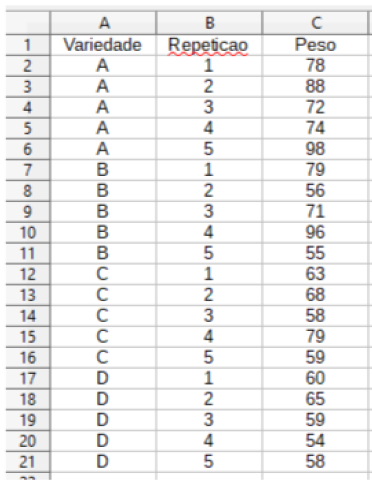
\includegraphics[width=0.8\linewidth]{delimexp0} 

}

\caption{Variedades de pera separadas por grupos em faixas de peso e repetição}\label{fig:unnamed-chunk-2}
\end{figure}

Existe diferença significativa entre as variedades de pera, considerando o peso médio dos frutos de cada variedade?

Para responder esta pergunta, utilizamos a Análise de Variância (ANOVA).

No software RStudio:

Criar o arquivo acima em planilha eletrônica. Nomear como DIC e salvar em formato .xls.

Importar no RStudio:

\begin{Shaded}
\begin{Highlighting}[]
\KeywordTok{library}\NormalTok{(readxl)}
\NormalTok{url <-}\StringTok{ "https://github.com/Smolski/livroavancado/raw/master/dic.xls"}
\NormalTok{destfile <-}\StringTok{ "dic.xls"}
\NormalTok{curl}\OperatorTok{::}\KeywordTok{curl_download}\NormalTok{(url, destfile)}
\NormalTok{DIC <-}\StringTok{ }\KeywordTok{read_excel}\NormalTok{(destfile)}
\KeywordTok{attach}\NormalTok{(DIC)}
\end{Highlighting}
\end{Shaded}

O comando que gera a análise de variância é o \texttt{aov()} e o comando que exibe o quadro da ANOVA é o \texttt{anova}. Então, podemos gerar o quadro da análise de uma são vez associando os dois comandos.

\begin{Shaded}
\begin{Highlighting}[]
\NormalTok{anova=}\KeywordTok{aov}\NormalTok{(Peso}\OperatorTok{~}\NormalTok{Variedade)}
\KeywordTok{summary}\NormalTok{(anova)}
\end{Highlighting}
\end{Shaded}

\begin{verbatim}
            Df Sum Sq Mean Sq F value Pr(>F)  
Variedade    3   1414     471    3.78  0.032 *
Residuals   16   1997     125                 
---
Signif. codes:  0 '***' 0.001 '**' 0.01 '*' 0.05 '.' 0.1 ' ' 1
\end{verbatim}

Hipóteses estatísticas:

\begin{itemize}
\tightlist
\item
  H\(_0\): ti \(=\) 0 (as médias dos tratamentos nãao diferem entre si)
\item
  H\(_1\): ti \(\neq\) 0 (existe, no mínimo, uma diferença entre as médias dos tratamentos)
\end{itemize}

Como p = 0,0319 (0,01 \(\leq\) p ``menor ou igual a'' 0,05), rejeita-se H\(_0\) com nível de significância de 5\% e conclui-se que existe diferença significativa entre as médias dos tratamentos.

Para saber quais as médias que diferem, utilizamos o teste de Tukey.

\begin{Shaded}
\begin{Highlighting}[]
\KeywordTok{attach}\NormalTok{(DIC)}
\end{Highlighting}
\end{Shaded}

\begin{verbatim}
The following objects are masked from DIC (pos = 3):

    Peso, Repeticao, Variedade
\end{verbatim}

\begin{Shaded}
\begin{Highlighting}[]
\KeywordTok{TukeyHSD}\NormalTok{(anova,}\KeywordTok{as.factor}\NormalTok{(}\StringTok{"Variedade"}\NormalTok{),}\DataTypeTok{ordered=}\OtherTok{TRUE}\NormalTok{)}
\end{Highlighting}
\end{Shaded}

\begin{verbatim}
  Tukey multiple comparisons of means
    95% family-wise confidence level
    factor levels have been ordered

Fit: aov(formula = Peso ~ Variedade)

$Variedade
    diff     lwr   upr  p adj
C-D  6.2 -14.016 26.42 0.8164
B-D 12.2  -8.016 32.42 0.3429
A-D 22.8   2.584 43.02 0.0245
B-C  6.0 -14.216 26.22 0.8303
A-C 16.6  -3.616 36.82 0.1282
A-B 10.6  -9.616 30.82 0.4602
\end{verbatim}

Para que o RStudio apresente uma tabela com as médias e letras indicando quais as médias que diferiram, devemos instalar o pacote \texttt{agricolae}.

\begin{Shaded}
\begin{Highlighting}[]
\KeywordTok{library}\NormalTok{(agricolae)}
\KeywordTok{HSD.test}\NormalTok{(anova,}\KeywordTok{as.factor}\NormalTok{(}\StringTok{"Variedade"}\NormalTok{),}\DataTypeTok{console=}\OtherTok{TRUE}\NormalTok{)}
\end{Highlighting}
\end{Shaded}

\begin{verbatim}

Study: anova ~ as.factor("Variedade")

HSD Test for Peso 

Mean Square Error:  124.8 

Variedade,  means

  Peso    std r Min Max
A 82.0 10.863 5  72  98
B 71.4 17.097 5  55  96
C 65.4  8.562 5  58  79
D 59.2  3.962 5  54  65

Alpha: 0.05 ; DF Error: 16 
Critical Value of Studentized Range: 4.046 

Minimun Significant Difference: 20.22 

Treatments with the same letter are not significantly different.

  Peso groups
A 82.0      a
B 71.4     ab
C 65.4     ab
D 59.2      b
\end{verbatim}

*Médias dos tratamentos não seguidas por mesma letra diferem pelo teste de Tukey, ao nível de 5\% de significância.

Conclusão: A variedade de pera A apresentou o maior peso médio dos frutos, que não diferiu significativamente do peso médio das variedades B e C. A variedade de pera D apresentou o menor peso médio dos frutos, que não diferiu significativamente do peso médio das variedades B e C. As variedades B e C apresentaram peso médio dos frutos intermediário.

\begin{Shaded}
\begin{Highlighting}[]
\KeywordTok{attach}\NormalTok{(DIC)}
\end{Highlighting}
\end{Shaded}

\begin{verbatim}
The following objects are masked from DIC (pos = 4):

    Peso, Repeticao, Variedade
\end{verbatim}

\begin{verbatim}
The following objects are masked from DIC (pos = 5):

    Peso, Repeticao, Variedade
\end{verbatim}

\begin{Shaded}
\begin{Highlighting}[]
\KeywordTok{boxplot}\NormalTok{(Peso}\OperatorTok{~}\NormalTok{Variedade)}
\end{Highlighting}
\end{Shaded}

\begin{center}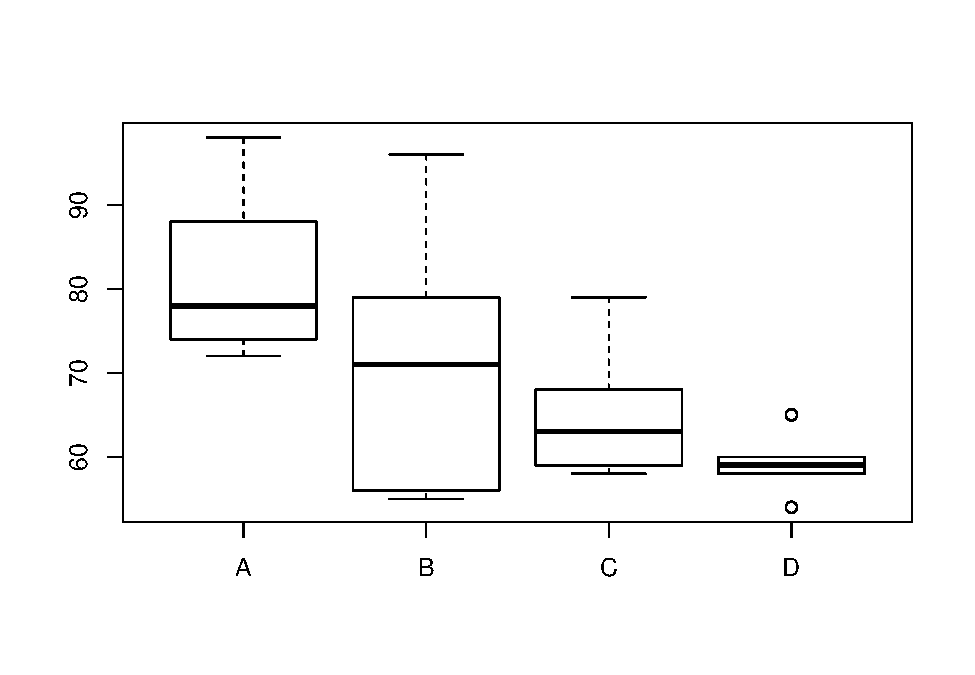
\includegraphics[width=0.8\linewidth]{index_files/figure-latex/unnamed-chunk-7-1} \end{center}

\begin{Shaded}
\begin{Highlighting}[]
\KeywordTok{boxplot}\NormalTok{(Peso}\OperatorTok{~}\NormalTok{Variedade,}\DataTypeTok{xlab=}\StringTok{"Variedade"}\NormalTok{,}\DataTypeTok{ylab=}\StringTok{"Peso"}\NormalTok{)}
\end{Highlighting}
\end{Shaded}

\begin{center}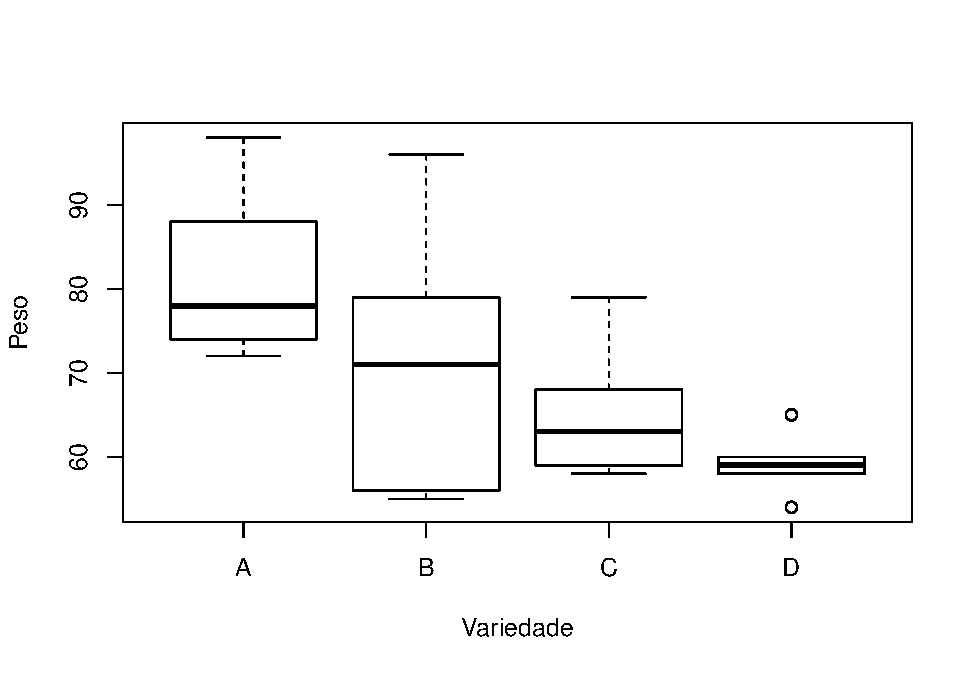
\includegraphics[width=0.8\linewidth]{index_files/figure-latex/unnamed-chunk-7-2} \end{center}

\begin{Shaded}
\begin{Highlighting}[]
\KeywordTok{tapply}\NormalTok{(Peso,Variedade,mean)}
\end{Highlighting}
\end{Shaded}

\begin{verbatim}
   A    B    C    D 
82.0 71.4 65.4 59.2 
\end{verbatim}

\begin{Shaded}
\begin{Highlighting}[]
\KeywordTok{tapply}\NormalTok{(Peso,Variedade,sd)}
\end{Highlighting}
\end{Shaded}

\begin{verbatim}
     A      B      C      D 
10.863 17.097  8.562  3.962 
\end{verbatim}

\begin{Shaded}
\begin{Highlighting}[]
\NormalTok{residuos=}\KeywordTok{residuals}\NormalTok{(anova)}
\NormalTok{ajustados=}\KeywordTok{fitted}\NormalTok{(anova)}
\KeywordTok{plot}\NormalTok{(ajustados,residuos)}
\KeywordTok{abline}\NormalTok{(}\DataTypeTok{h=}\DecValTok{0}\NormalTok{)}
\end{Highlighting}
\end{Shaded}

\begin{center}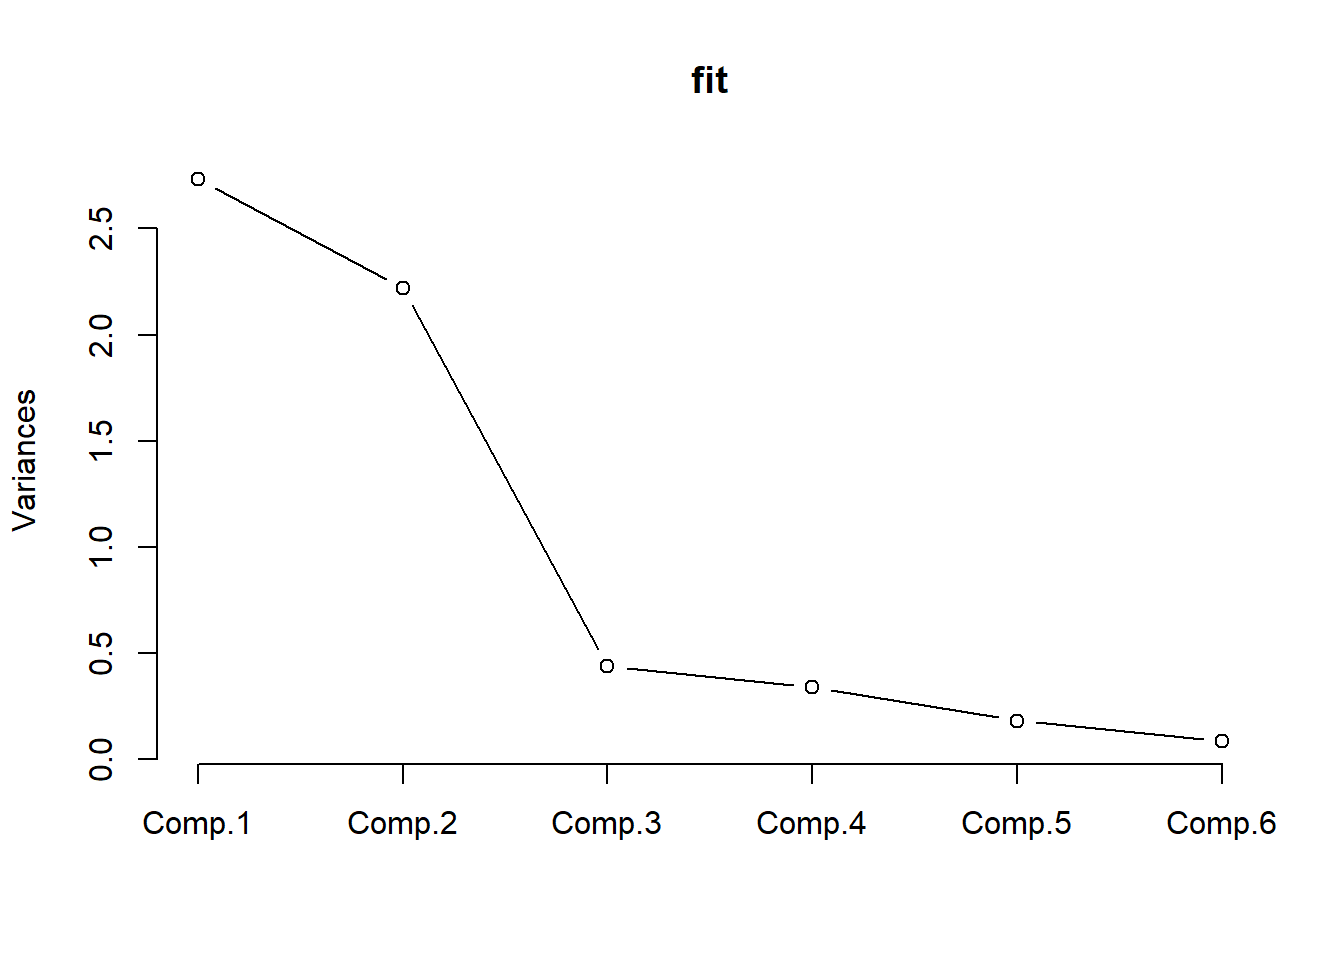
\includegraphics[width=0.8\linewidth]{index_files/figure-latex/unnamed-chunk-9-1} \end{center}

\begin{Shaded}
\begin{Highlighting}[]
\KeywordTok{qqnorm}\NormalTok{(residuos)}
\KeywordTok{qqline}\NormalTok{(residuos)}
\end{Highlighting}
\end{Shaded}

\begin{center}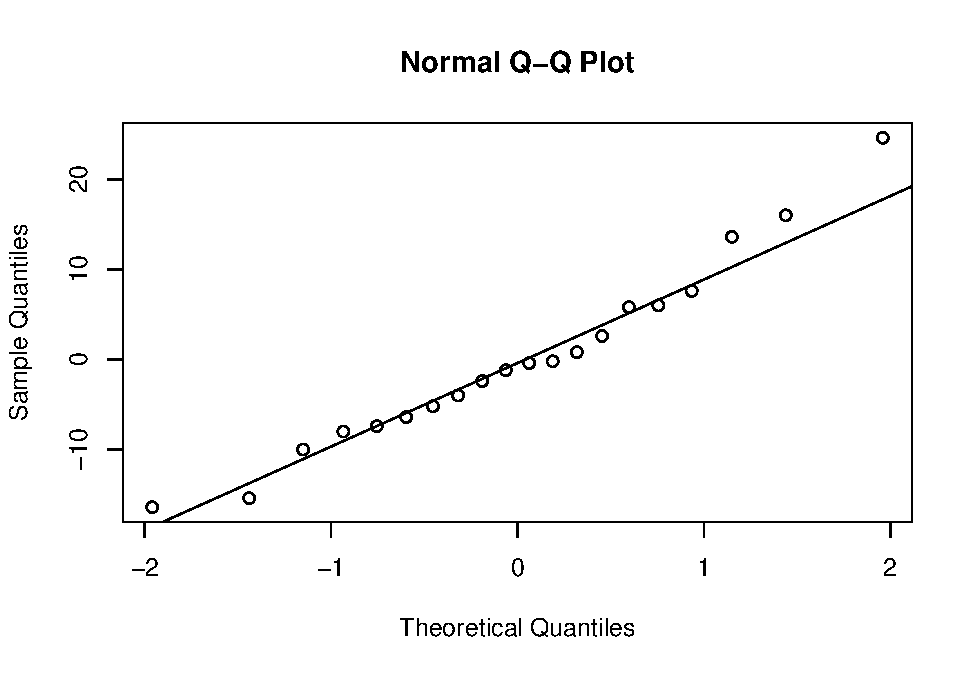
\includegraphics[width=0.8\linewidth]{index_files/figure-latex/unnamed-chunk-10-1} \end{center}

\hypertarget{delineamento-blocos-casualizados-dbc}{%
\section{Delineamento Blocos Casualizados (DBC)}\label{delineamento-blocos-casualizados-dbc}}

É utilizado quando as unidades experimentais são heterogêneas. Os tratamentos são designados às unidades experimentais de forma casualizada, por meio de sorteio por blocos. Na área agrícola, é usado principalmente em áreas de campo e grandes animais.

\emph{Exemplo}: Uma Nutricionista elaborou 4 dietas e quer aplicá-las em 20 pessoas a fim detestar suas eficiências quanto à perda de peso. Porém ela notou que entre essas 20 pessoas existem 5 grupos de faixas iniciais de peso. Então, para aumentar a eficácia do teste ela separou os 20 indivíduos em 5 grupos de faixas de peso.

\begin{figure}[H]

{\centering 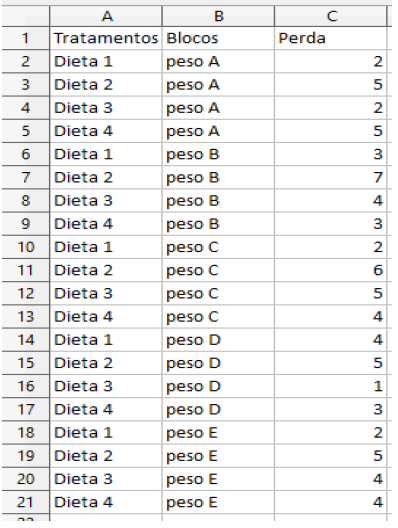
\includegraphics[width=0.8\linewidth]{delimexp1} 

}

\caption{Indivíduos separados por grupos em faixas de peso}\label{fig:unnamed-chunk-11}
\end{figure}

Criar o arquivo acima em planilha eletrônica. Nomear como DBC e salvar em formato .xls.

Importar no RStudio:

\begin{Shaded}
\begin{Highlighting}[]
\KeywordTok{require}\NormalTok{(readxl)}
\NormalTok{url <-}\StringTok{ "https://github.com/Smolski/livroavancado/raw/master/dbc.xls"}
\NormalTok{destfile <-}\StringTok{ "dbc.xls"}
\NormalTok{curl}\OperatorTok{::}\KeywordTok{curl_download}\NormalTok{(url, destfile)}
\NormalTok{DBC  <-}\StringTok{ }\KeywordTok{read_excel}\NormalTok{(destfile)}

\KeywordTok{attach}\NormalTok{(DBC)}
\NormalTok{anova=}\KeywordTok{aov}\NormalTok{(Perda}\OperatorTok{~}\NormalTok{Tratamentos}\OperatorTok{+}\NormalTok{Blocos)}
\KeywordTok{summary}\NormalTok{(anova)}
\end{Highlighting}
\end{Shaded}

\begin{verbatim}
            Df Sum Sq Mean Sq F value Pr(>F)   
Tratamentos  3   25.2     8.4    6.00 0.0097 **
Blocos       4    3.2     0.8    0.57 0.6885   
Residuals   12   16.8     1.4                  
---
Signif. codes:  0 '***' 0.001 '**' 0.01 '*' 0.05 '.' 0.1 ' ' 1
\end{verbatim}

Hipóteses estatísticas:

\begin{itemize}
\tightlist
\item
  H\(_0\): ti \(=\) 0 (as médias dos tratamentos não diferem entre si)
\item
  H\(_1\): ti \(\neq\) 0 (existe, no mínimo, uma diferença entre as médias dos tratamentos)
\end{itemize}

Como p = 0,00973 (p \(\leq\) 0,01), rejeita-se H\(_0\) com nível de significância de 1\% e conclui-se que existe diferença significativa entre as médias dos tratamentos.

\begin{itemize}
\tightlist
\item
  H\(_0\): \(\sigma\)\textsuperscript{2} blocos \(=\) 0
\item
  H\(_1\): \(\sigma\)\textsuperscript{2} blocos \(\leq\) 0
\end{itemize}

Como p \(=\) 0,68854 (p \(\leq\) 0,05), não rejeita-se H\(_0\) e conclui-se que a variância entre os blocos não é significativa.

\begin{Shaded}
\begin{Highlighting}[]
\KeywordTok{attach}\NormalTok{(DBC)}
\KeywordTok{HSD.test}\NormalTok{(anova,}\KeywordTok{as.factor}\NormalTok{(}\StringTok{"Tratamentos"}\NormalTok{),}\DataTypeTok{console=}\OtherTok{TRUE}\NormalTok{)}
\end{Highlighting}
\end{Shaded}

\begin{verbatim}

Study: anova ~ as.factor("Tratamentos")

HSD Test for Perda 

Mean Square Error:  1.4 

Tratamentos,  means

        Perda    std r Min Max
Dieta 1   2.6 0.8944 5   2   4
Dieta 2   5.6 0.8944 5   5   7
Dieta 3   3.2 1.6432 5   1   5
Dieta 4   3.8 0.8367 5   3   5

Alpha: 0.05 ; DF Error: 12 
Critical Value of Studentized Range: 4.199 

Minimun Significant Difference: 2.222 

Treatments with the same letter are not significantly different.

        Perda groups
Dieta 2   5.6      a
Dieta 4   3.8     ab
Dieta 3   3.2      b
Dieta 1   2.6      b
\end{verbatim}

Médias dos tratamentos não seguidas por mesma letra diferem pelo teste de Tukey, ao nível de 5\% de significância.

Conclusão: A dieta que resultou na maior perda de peso foi a dieta 2, que não diferiu da dieta 4. A dieta que resultou na menor perda de peso foi a dieta 1, que não diferiu das dietas 3 e 4.

Medidas descritivas com a variável resposta:

\begin{Shaded}
\begin{Highlighting}[]
\KeywordTok{boxplot}\NormalTok{(Perda}\OperatorTok{~}\NormalTok{Tratamentos)}
\end{Highlighting}
\end{Shaded}

\begin{center}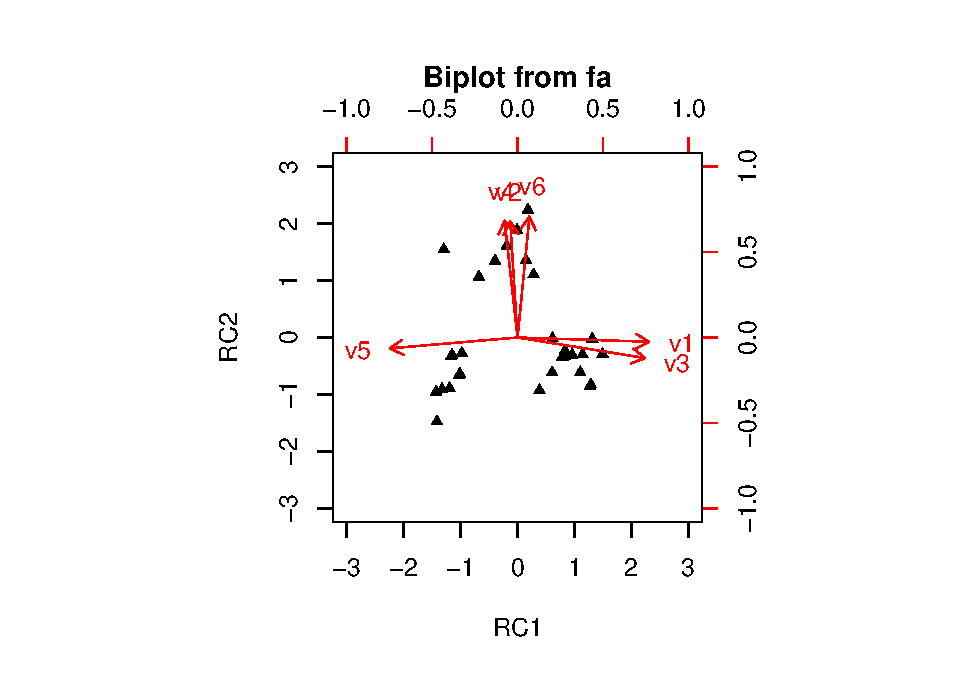
\includegraphics[width=0.8\linewidth]{index_files/figure-latex/unnamed-chunk-14-1} \end{center}

\begin{Shaded}
\begin{Highlighting}[]
\KeywordTok{boxplot}\NormalTok{(Perda}\OperatorTok{~}\NormalTok{Tratamentos,}\DataTypeTok{xlab=}\StringTok{"Tratamentos"}\NormalTok{,}\DataTypeTok{ylab=}\StringTok{"Perda"}\NormalTok{)}
\end{Highlighting}
\end{Shaded}

\begin{center}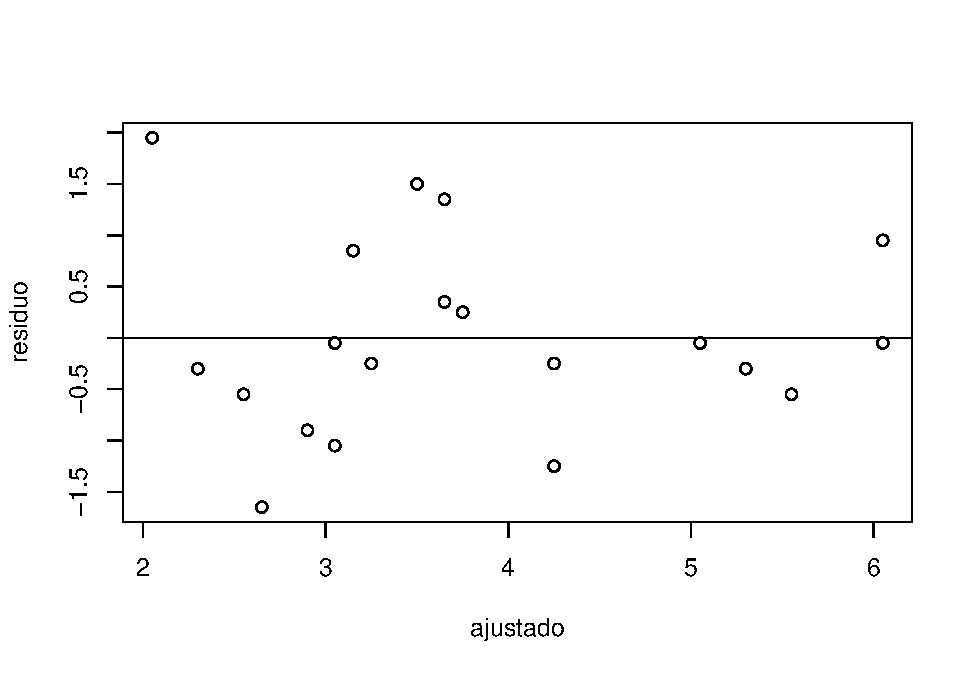
\includegraphics[width=0.8\linewidth]{index_files/figure-latex/unnamed-chunk-15-1} \end{center}

\begin{Shaded}
\begin{Highlighting}[]
\KeywordTok{tapply}\NormalTok{(Perda,Tratamentos,mean)}
\end{Highlighting}
\end{Shaded}

\begin{verbatim}
Dieta 1 Dieta 2 Dieta 3 Dieta 4 
    2.6     5.6     3.2     3.8 
\end{verbatim}

\begin{Shaded}
\begin{Highlighting}[]
\KeywordTok{tapply}\NormalTok{(Perda,Tratamentos,sd)}
\end{Highlighting}
\end{Shaded}

\begin{verbatim}
Dieta 1 Dieta 2 Dieta 3 Dieta 4 
 0.8944  0.8944  1.6432  0.8367 
\end{verbatim}

\begin{Shaded}
\begin{Highlighting}[]
\NormalTok{residuo=}\KeywordTok{residuals}\NormalTok{(anova)}
\NormalTok{ajustado=}\KeywordTok{fitted}\NormalTok{(anova)}
\KeywordTok{plot}\NormalTok{(ajustado,residuo)}
\KeywordTok{abline}\NormalTok{(}\DataTypeTok{h=}\DecValTok{0}\NormalTok{)}
\end{Highlighting}
\end{Shaded}

\begin{center}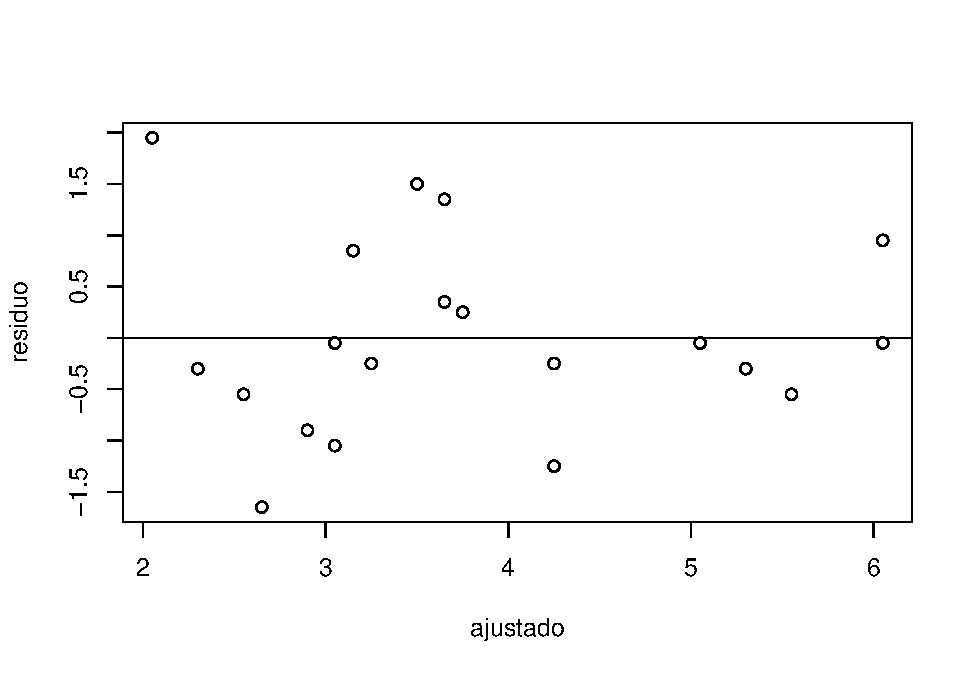
\includegraphics[width=0.8\linewidth]{index_files/figure-latex/unnamed-chunk-17-1} \end{center}

\begin{Shaded}
\begin{Highlighting}[]
\KeywordTok{qqnorm}\NormalTok{(residuo)}
\KeywordTok{qqline}\NormalTok{(residuo)}
\end{Highlighting}
\end{Shaded}

\begin{center}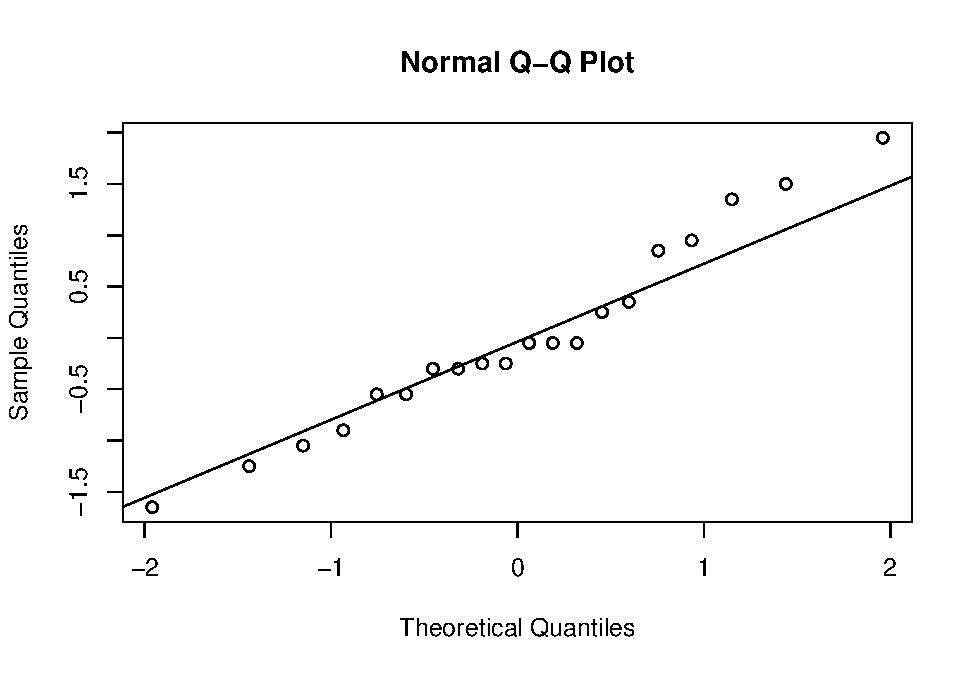
\includegraphics[width=0.8\linewidth]{index_files/figure-latex/unnamed-chunk-18-1} \end{center}

\hypertarget{analise-fatorial}{%
\chapter{Análise Fatorial}\label{analise-fatorial}}

\emph{Denize Ivete Reis}

A análise fatorial é um método estatístico utilizado para descrever a variabilidade entre variáveis observadas e possivelmente correlacionadas em termos de um número potencialmente menor de variáveis não observadas chamadas fatores.

Assim, é possível que as variaçõess de três ou quatro variáveis observadas possam ser explicadas por somente um fator, o que evidencia a utilidade da análise fatorial para descrever um conjunto de dados utilizando para isso apenas alguns fatores.

Diferentemente da análise de variância, regressão e análise discriminante, onde uma das variáveis é identificada como a variável dependente, examina-se todo o conjunto de relações interdependentes entre variáveis.

\begin{figure}[H]

{\centering 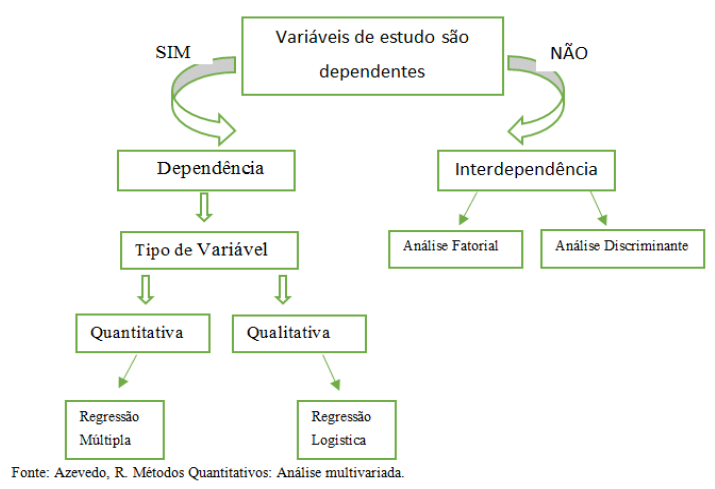
\includegraphics[width=0.8\linewidth]{anfat1} 

}

\caption{Processo de análise de variáveis}\label{fig:unnamed-chunk-19}
\end{figure}

A análise fatorial aborda o problema de analisar a estrutura das inter-relações (correlações) entre um grande número de variáveis (escores de testes, itens de testes, respostas de questionários), definindo um conjunto de dimensões latentes comuns, chamados fatores. Então, a análise fatorial, permite primeiro identificar as dimensões separadas da estrutura e então determinar o grau em que cada variável é explicada por cada dimensão. Uma vez que essas dimensões e a explicação da cada variável estejam determinadas, os dois principais usos da análise fatorial podem ser conseguidos:

\begin{itemize}
\item
  \textbf{Resumo}: ao resumir os dados, a análise fatorial obtém dimensões latentes que, quando interpretadas e compreendidas, descrevem os dados em um núumero muito menor de conceitos do que as variáveis individuais originais.
\item
  \textbf{Redução de dados}: pode ser obtida calculando escores para cada dimensão latente e substituindo as variáveis originais pelos mesmos.
\end{itemize}

As técnicas analíticas fatoriais podem ser classificadas quanto aos seus objetivos como \textbf{exploratória} ou \textbf{confirmatória}. Exploratória, útil na busca da estrutura em um conjunto de variáveis ou como um método de redução de dados. Sob esta perspectiva, as técnicas analíticas fatoriais ``consideram o que os dados oferecem''e não estabelecem restriçoes \emph{a priori} sobre o número de componentes a serem extraídos. O uso da análise fatorial em situações, que se deseja testar hipóteses envolvendo questões sobre, quais variáveis deveriam ser agrupadasem fator ou número exato de fatores, por exemplo, a análise fatorial desempenha um papel confirmatório, ou seja, avalia o grau em que os dados satisfazem a estrutura esperada.

Exemplo: em maketing, fatores associados às características do produto, clientes e até mesmo da organização.

Em estudos visando analisar o inter-relacionamento e o agrupamento de indivíduos, cidade ou regiões em grupos homogêneos em relação à mobilidade, preferências pessoais, condições de desenvolvimento, entre outras variáveis.

\hypertarget{pressupostos}{%
\section{Pressupostos}\label{pressupostos}}

A análise fatorial clássica exige que alguns pressupostos sejam satisfeitos, quais sejam (MALHOTRA, 2001):

\begin{enumerate}
\def\labelenumi{\alph{enumi}.}
\item
  Normalidade dos dados: apesar deste pressuposto não ser crítico quando a estimação é realizada por mínimos quadrados ordinários, a exigência de normalidade auxilia na análise, evitando possíveis assimetrias e a presença de \emph{outliers}.
\item
  Variáveis quantitativas medidas em escala Intervalar ou de Razão. Esse pressuposto é crítico, pois a análise deve ser realizada com variáveis quantitatias e, frequentemente, alguns estudos são realizados utilizando variáveis ordinais (as quaiss são qualitativas) na análise fatorial clássica (o que é errado de muitas maneiras).
\item
  Como diretriz inicial deve haver ao menos quatro a cinco vezes mais observações do que variáveis.
\end{enumerate}

\hypertarget{estatisticas-associadas-a-analise-fatorial}{%
\section{Estatísticas Associadas a Análise Fatorial}\label{estatisticas-associadas-a-analise-fatorial}}

Em geral, as estatísticas utilizadas no processo de análise fatorial são (AAKER-KUMARDAY, 2001):

\begin{itemize}
\item
  Teste de esfericidade de Bartlett: estatística de teste usada para examinar a hipótese de que as variáveis não sejam correlacionadas na população, ou seja, a matriz de correlação da população é uma matriz identidade onde cada variável se correlaciona perfeitamente com ela própria (r=1), mas não apresenta correlação com as outras variáveis (r=0).
\item
  Matriz de correlação: o triângulo inferior da matriz exibe as correlações simples, r, entre todos os pares possíveis de variáveis incluídas na análise, enquanto os elementos da diagonal, que são todos iguais a 1, em geral são omitidos.
\item
  Comunalidade: porção da variância que uma variável compartilha com todas as outras variáveis consideradas, sendo também a proporção de variância explicada pelos fatores comuns.
\item
  Autovalor: representa a variância total explicada por cada fator.
\item
  Cargas fatoriais: correlação simples entre as variáveis e os fatores.
\item
  Gráfico das cargas dos fatores: gráfico das variáveis originais utilizando as cargas fatoriais como ordenadas.
\item
  Matriz de fatores ou matriz principal: contém as cargas fatoriais de todos as variáveis em todos os fatores extraídos.
\item
  Escores fatoriais: escores compostos estimados para cada entrevistado nos fatores derivados.
\item
  Medida de adequacidade da amostra de Kaiser-Meyer-Olkin (KMO): é o índice usado para avaliar a adequacidade da análise fatorial. Valores altos (entre 0,5 e 1,0) indicam que a análise fatorial é apropriada. Valores abaixo de 0,5 indicam que a análise fatorial pode ser inadequada.
\item
  Percentagem de variância: percentagem da variância total atribuída a cada fator.
\item
  Resíduos: diferenças entre as correlações observadas, dadas na matriz de correlação de entrada (input) e as correlações reproduzidas, conforme estimadas pela matriz de fatores.
\item
  Scree plot: gráfico dos autovalores versus número de fatores por ordem de extração.
\end{itemize}

Exemplo 1:

(MALHOTRA, 2001) Suponhamos que um pesquisador queira avaliar os benefícios que os consumidores esperam de um dentifrício. Foi entrevistada uma amostra de 30 pessoas em um supermercado, para que indicassem seu grau de concordância com as seguintes afirmações, utilizando uma escala de 7 pontos (1= discordância total, 7 =concordância total).

\begin{itemize}
\tightlist
\item
  V1: É importante comprar um creme dental que evite cáries.
\item
  V2: Gosto de um creme dental que clareie os dentes.
\item
  V3: Um creme dental deve fortificar as gengivas.
\item
  V4: Prefiro um creme dental que refresque o hálito.
\item
  V5: Manter os dentes sadios não é uma vantagem importante de um creme dental.
\item
  V6: O aspecto mais importante na compra de um creme dental é tornar os dentes atraentes.
\end{itemize}

Inicialmente podemos explorar algumas estatísticas descritivas relacionadas às variáveis pesquisadas, utilizando a função \texttt{summary}:

\begin{Shaded}
\begin{Highlighting}[]
\KeywordTok{require}\NormalTok{(readxl)}

\NormalTok{url <-}\StringTok{ "https://github.com/Smolski/livroavancado/raw/master/creme_dental_exemplo1.xlsx"}
\NormalTok{destfile <-}\StringTok{ "creme_dental_exemplo1.xlsx"}
\NormalTok{curl}\OperatorTok{::}\KeywordTok{curl_download}\NormalTok{(url, destfile)}
\NormalTok{creme_dental_exemplo1 <-}\StringTok{ }\KeywordTok{read_excel}\NormalTok{(destfile)}

\KeywordTok{attach}\NormalTok{(creme_dental_exemplo1)}
\KeywordTok{summary}\NormalTok{(creme_dental_exemplo1)}
\end{Highlighting}
\end{Shaded}

\begin{verbatim}
       v1             v2            v3            v4            v5     
 Min.   :1.00   Min.   :2.0   Min.   :1.0   Min.   :2.0   Min.   :1.0  
 1st Qu.:2.00   1st Qu.:3.0   1st Qu.:2.0   1st Qu.:3.0   1st Qu.:2.0  
 Median :4.00   Median :4.0   Median :4.0   Median :4.0   Median :3.5  
 Mean   :3.93   Mean   :3.9   Mean   :4.1   Mean   :4.1   Mean   :3.5  
 3rd Qu.:6.00   3rd Qu.:5.0   3rd Qu.:6.0   3rd Qu.:5.0   3rd Qu.:5.0  
 Max.   :7.00   Max.   :7.0   Max.   :7.0   Max.   :7.0   Max.   :7.0  
       v6      
 Min.   :2.00  
 1st Qu.:3.00  
 Median :4.00  
 Mean   :4.17  
 3rd Qu.:4.75  
 Max.   :7.00  
\end{verbatim}

\hypertarget{passos-da-analise-fatorial}{%
\section{Passos da Análise Fatorial}\label{passos-da-analise-fatorial}}

Basicamente, os seguintes passos conduzem a análise fatorial: entrada de dados, cálculo das correlações entre as variáveis, extração inicial dos fatores e a rotação da matriz.

\hypertarget{construcao-da-matriz-de-correlacao}{%
\subsection{Construção da Matriz de Correlação}\label{construcao-da-matriz-de-correlacao}}

Entrada de Dados (BASE): os dados de entrada da análise fatorial geralmente tomam a forma de um conjunto de valores de variáveis para cada objeto ou indivíduo na amostra. Toda matriz, cujos componentes ofereçam uma medida de similaridade entre variáveis, pode ser passível de análise fatorial. A medida de similaridade não precisa ser uma correlação, embora, geralmente, ou seja:

Para que a análise fatorial seja adequada, as variáveis devem ser correlacionadas. Espera-se também que as variáveis altamente correlacionadas umas com as outras se correlacionem também com o(s) mesmo(s) fatore(s).

Note que existem correlações amostrais positivas e negativas relativamente elevadas entre V1 (prevenção de cáries), V3 (gengivas fortes) e V5 (dentes sadios). Espera-se que essas variáveis se relacionem com o mesmo conjunto de fatores. Verificam-se também correlações relativamente elevadas entre V2 (clareie os dentes), V4 (hálito puro) e V6 (dentes atraentes). Essas variáveis também devem correlacionar-se com os mesmos fatores.

\begin{Shaded}
\begin{Highlighting}[]
\NormalTok{matcor <-}\StringTok{ }\KeywordTok{cor}\NormalTok{(creme_dental_exemplo1)}
\KeywordTok{print}\NormalTok{(matcor, }\DataTypeTok{digits =} \DecValTok{2}\NormalTok{)}
\end{Highlighting}
\end{Shaded}

\begin{verbatim}
        v1     v2     v3      v4      v5      v6
v1  1.0000 -0.053  0.873 -0.0862 -0.8576  0.0042
v2 -0.0532  1.000 -0.155  0.5722  0.0197  0.6405
v3  0.8731 -0.155  1.000 -0.2478 -0.7778 -0.0181
v4 -0.0862  0.572 -0.248  1.0000 -0.0066  0.6405
v5 -0.8576  0.020 -0.778 -0.0066  1.0000 -0.1364
v6  0.0042  0.640 -0.018  0.6405 -0.1364  1.0000
\end{verbatim}

\begin{Shaded}
\begin{Highlighting}[]
\KeywordTok{require}\NormalTok{(corrplot)}
\end{Highlighting}
\end{Shaded}

\begin{verbatim}
Carregando pacotes exigidos: corrplot
\end{verbatim}

\begin{verbatim}
corrplot 0.84 loaded
\end{verbatim}

\begin{Shaded}
\begin{Highlighting}[]
\KeywordTok{corrplot}\NormalTok{(matcor, }\DataTypeTok{method=}\StringTok{"circle"}\NormalTok{)}
\end{Highlighting}
\end{Shaded}

\begin{center}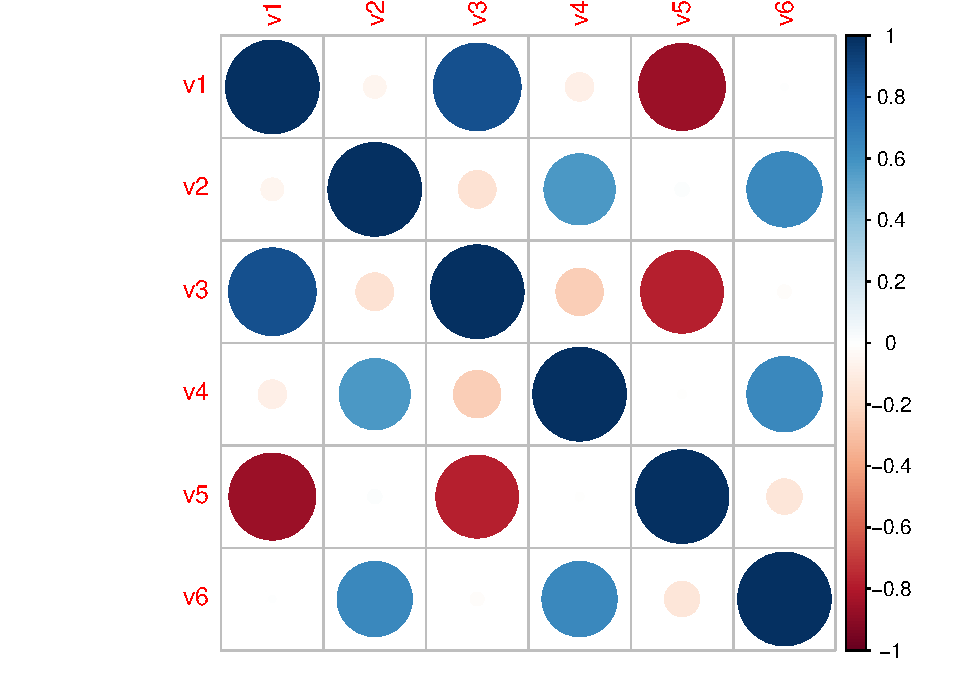
\includegraphics[width=0.8\linewidth]{index_files/figure-latex/unnamed-chunk-22-1} \end{center}

Na figura acima, as correlações estão em cor azul porque são positivas, com tons mais fortes para as correlações mais altas.

Para testar a conveniência do modelo fatorial pode-se aplicar o teste de esfericidade de Bartlett para testar a hipótese nula, de que as variáveis não sejam correlacionadas na população.
Um valor elevado da estatística de teste favorece a rejeição da hipótese nula.

Também, a medida de adequacidade da amostra de Kaiser-Meyer-Olkin (KMO) compara as magnitudes dos coeficientes de correlação observados com as magnitudes dos coeficientes de
correlação parcial. Pequenos valores de KMO indicam que as correlações entre os pares de variáveis não podem ser explicadas por outras variáveis, indicando que a análise fatorial não é adequada.

Hipóteses:

Ho: A matriz de correlação da população é uma matriz identidade, ou seja as variáveis não são correlacionadas na população.

H\(_1\): A matriz de correlação da população não é uma matriz identidade, ou seja as variáveis são correlacionadas na população.

\begin{Shaded}
\begin{Highlighting}[]
\CommentTok{#install.packages("psych")}
\KeywordTok{require}\NormalTok{(psych)}
\end{Highlighting}
\end{Shaded}

\begin{verbatim}
Carregando pacotes exigidos: psych
\end{verbatim}

\begin{Shaded}
\begin{Highlighting}[]
\KeywordTok{cortest.bartlett}\NormalTok{(creme_dental_exemplo1)}
\end{Highlighting}
\end{Shaded}

\begin{verbatim}
R was not square, finding R from data
\end{verbatim}

\begin{verbatim}
$chisq
[1] 111.3

$p.value
[1] 9.017e-17

$df
[1] 15
\end{verbatim}

Veja que a hipótese nula de que a matriz de correlação da população seja uma matriz identidade é rejeitada pelo teste de esfericidade de Bartlett. A estatística qui-quadrado aproximada
é 111,314, com 15 graus de liberdade, significativa ao nível de 0,05.

\begin{Shaded}
\begin{Highlighting}[]
\KeywordTok{KMO}\NormalTok{(creme_dental_exemplo1)}
\end{Highlighting}
\end{Shaded}

\begin{verbatim}
Kaiser-Meyer-Olkin factor adequacy
Call: KMO(r = creme_dental_exemplo1)
Overall MSA =  0.66
MSA for each item = 
  v1   v2   v3   v4   v5   v6 
0.62 0.70 0.68 0.64 0.77 0.56 
\end{verbatim}

A estatística KMO maior que 0,5 também concorda quanto ao fato de que a análise fatorial pode ser considerada uma técnica apropriada para analisar a matriz de correlação.

\hypertarget{metodo-de-analise-fatorial}{%
\subsection{Método de Análise Fatorial}\label{metodo-de-analise-fatorial}}

As duas abordagens básicas são a análise de componentes principais (ACP) e a análise fatorial (AFC) comum ou análise fatorial exploratória (AFE), embora existam diferentes métodos
de extração de fatores da matriz de correlações, que de forma geral, são métodos numericamente complexos. Na análise de componentes principais, o objetivo da extração de fatores é encontrar um conjunto de fatores que formem uma combinação linear das variáveis originais ou da matriz de correlações. Assim, se as variáveis X1 , X2 , X3 , \ldots{} , Xn são altamente correlacionadas entre si, elas serão combinadas para formar um fator, e assim, sucessivamente, com todas as demais variáveis
da matriz de correlação.

A análise fatorial exploratória pode trazer informações importantes sobre a estrutura multivariada de um instrumento de mensuração, identificando os construtos teóricos.

O segundo objetivo da analise fatorial exploratória está relacionado à redução de dados e descoberta de ponderações ótimas para as variáveis mensuradas, de forma que um grande conjunto de variáveis possa ser reduzido a um conjunto menor de índices sumários que tenham máxima variabilidade e fidedignidade. A redução de dados é especialmente possível pela aplicação da Análise dos Componentes Principais (ACP) e não pelo uso da analise fatorial comum (AFC), havendo uma diferença fundamental entre os dois métodos: a ACP trabalha com a variância total observada, enquanto a AFC trabalha somente com a variância partilhada dos itens (variância erro e variância única são excluídas) (LAROS, 2012).

Na AFC, os fatores são estimados para explicar as covariâncias entre as variáveis observadas, portanto os fatores são considerados como as causas das variáveis observadas. Já na ACP, os componentes são estimados para representar a variância das variáveis observadas de uma maneira tão econômica quanto possível. Os componentes principais são somas otimamente ponderadas das variáveis observadas, neste sentido, as variáveis observadas são consideradas as causas dos componentes principais (LAROS, 2012).

Assim, recomenda-se a ACP, quando o objetivo é determinar o número mínimo de fatores que respondem pela máxima variância nos dados, sendo os fatores chamados componentes principais (MALHOTRA, 2001).

Obs.:

cor = TRUE: as componentes principais serão geradas a partir da matriz de correlação.

cor = FALSE: as componentes principais serão geradas a partir da matriz de covariância.

\begin{Shaded}
\begin{Highlighting}[]
\NormalTok{fit<-}\KeywordTok{princomp}\NormalTok{(creme_dental_exemplo1,}\DataTypeTok{cor=}\OtherTok{TRUE}\NormalTok{)}
\NormalTok{fit}
\end{Highlighting}
\end{Shaded}

\begin{verbatim}
Call:
princomp(x = creme_dental_exemplo1, cor = TRUE)

Standard deviations:
Comp.1 Comp.2 Comp.3 Comp.4 Comp.5 Comp.6 
1.6526 1.4893 0.6645 0.5842 0.4274 0.2919 

 6  variables and  30 observations.
\end{verbatim}

\begin{Shaded}
\begin{Highlighting}[]
\KeywordTok{summary}\NormalTok{(fit)}
\end{Highlighting}
\end{Shaded}

\begin{verbatim}
Importance of components:
                       Comp.1 Comp.2 Comp.3  Comp.4  Comp.5 Comp.6
Standard deviation     1.6526 1.4893 0.6645 0.58417 0.42735 0.2919
Proportion of Variance 0.4552 0.3697 0.0736 0.05688 0.03044 0.0142
Cumulative Proportion  0.4552 0.8249 0.8985 0.95536 0.98580 1.0000
\end{verbatim}

A função \texttt{summary(fit)} mostra a aplicação da análise de componentes principais. O fator 1
responde por 45,52\% da variância total. Da mesma forma, o segundo fator responde por 36,97\% da
variância total, sendo que os dois primeiros fatores respondem por 82,49\% da variância total. Várias
considerações devem integrar a análise do núumero de fatores que devem ser usados na análise.

\hypertarget{determinacao-do-nuumero-de-fatores}{%
\subsection{Determinação do núumero de fatores}\label{determinacao-do-nuumero-de-fatores}}

A fim de reduzir as informações presentes nas variáveis originais, deve-se reduzir o número de fatores. Na literatura, diversos processos são sugeridos: determinação a priori, observação dos autovalores, representação gráfica (\textbf{scree plot}), testes de significância entre outros.

\hypertarget{determinacao-a-priori}{%
\subsubsection{Determinação a priori}\label{determinacao-a-priori}}

Quando o pesquisador, com base na experiência que apresentação em relação ao assunto,
decide quantos fatores deseja utilizar.

\hypertarget{autovalores}{%
\subsubsection{Autovalores}\label{autovalores}}

Como o autovalor representa a quantidade de variância associada ao fator, incluem-se
apenas os fatores com variância maior que 1.

\hypertarget{grafico-de-declive-scree-plot}{%
\subsubsection{\texorpdfstring{Gráfico de declive (\textbf{scree plot})}{Gráfico de declive (scree plot)}}\label{grafico-de-declive-scree-plot}}

Trata-se de uma representação gráfica dos autovalores associada ao número de fatores na
ordem de extração. O ponto em que a inclinação suaviza indica o número de fatores a ser usados,
que em geral é superior ao revelado pelos autovalores.

\hypertarget{percentagem-da-variancia}{%
\subsubsection{Percentagem da variância}\label{percentagem-da-variancia}}

Determina que o núumero de fatores extraídos seja de no mínimo 60\% da variância.

\hypertarget{teste-de-significancia}{%
\subsubsection{Teste de significância}\label{teste-de-significancia}}

É possível reter apenas os fatores estatisticamente significativos com base na significância estatística dos autovalores separados.

Abaixo vamos apresentar o \texttt{scree-plot}, em formato do gráfico de barras para o nosso exemplo

\begin{Shaded}
\begin{Highlighting}[]
\KeywordTok{screeplot}\NormalTok{(fit)}
\end{Highlighting}
\end{Shaded}

\begin{center}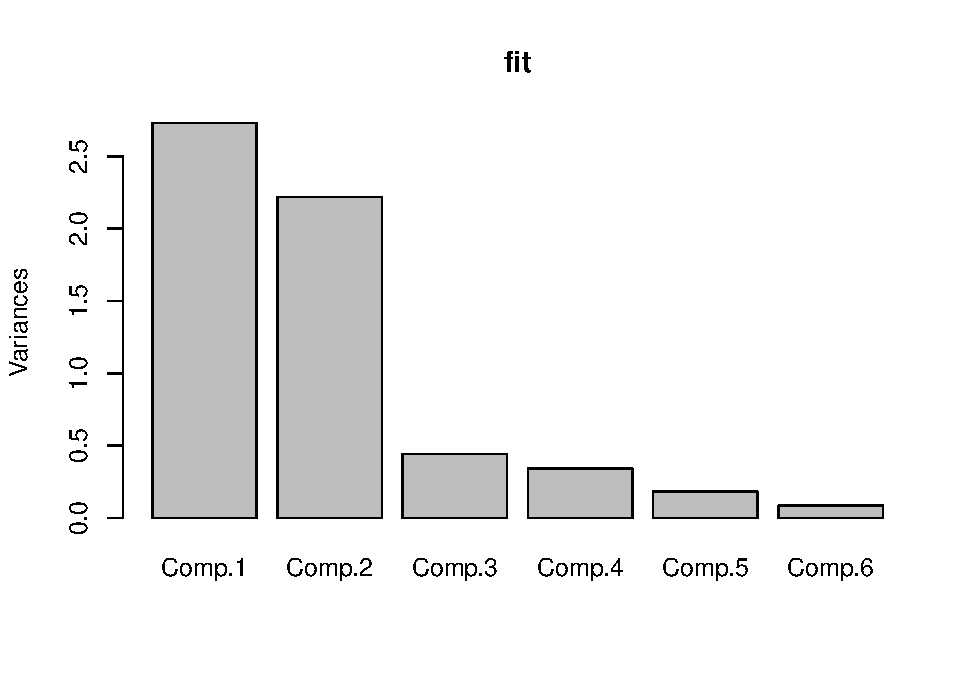
\includegraphics[width=0.8\linewidth]{index_files/figure-latex/unnamed-chunk-26-1} \end{center}

Note que as duas primeiras componentes, aparecem em destaque, ocorrendo uma ligeira suavização das alturas nas demais colunas.

\begin{Shaded}
\begin{Highlighting}[]
\KeywordTok{plot}\NormalTok{(fit,}\DataTypeTok{type=}\StringTok{"lines"}\NormalTok{)}
\end{Highlighting}
\end{Shaded}

\begin{center}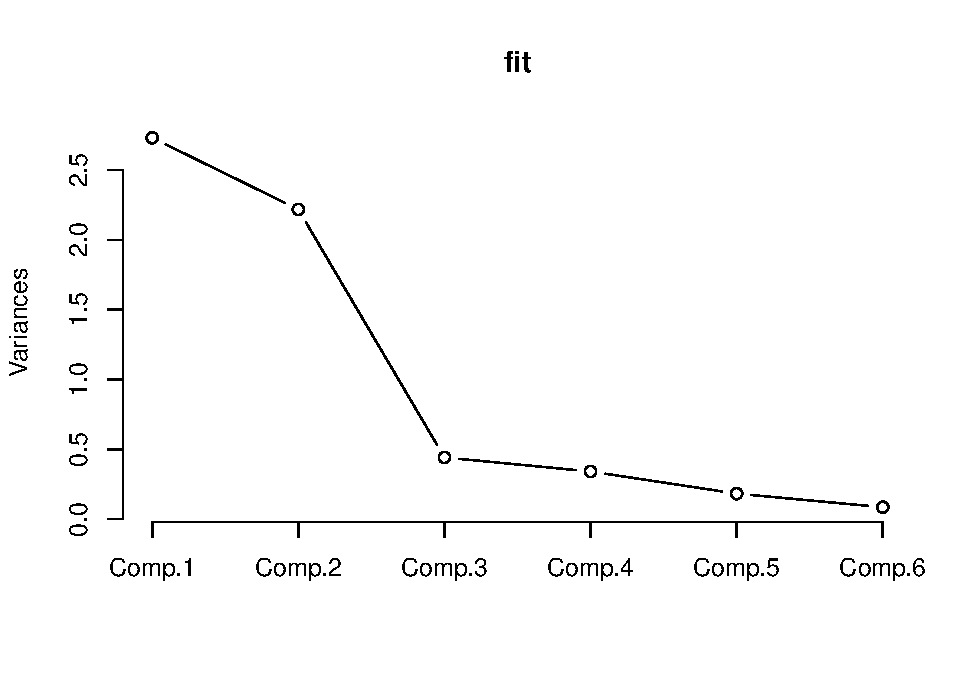
\includegraphics[width=0.8\linewidth]{index_files/figure-latex/unnamed-chunk-27-1} \end{center}

\hypertarget{analise-de-componentes-principais}{%
\subsection{Análise de Componentes Principais}\label{analise-de-componentes-principais}}

Rodando a Análise de Componentes Principais no R, temos:

\begin{Shaded}
\begin{Highlighting}[]
\NormalTok{PCAdente<-}\KeywordTok{principal}\NormalTok{(creme_dental_exemplo1, }\DataTypeTok{nfactors=}\DecValTok{2}\NormalTok{,}
                \DataTypeTok{n.obs=}\DecValTok{30}\NormalTok{,}\DataTypeTok{rotate=}\StringTok{"none"}\NormalTok{, }\DataTypeTok{scores=}\OtherTok{TRUE}\NormalTok{)}
\NormalTok{PCAdente}
\end{Highlighting}
\end{Shaded}

\begin{verbatim}
Principal Components Analysis
Call: principal(r = creme_dental_exemplo1, nfactors = 2, rotate = "none", 
    n.obs = 30, scores = TRUE)
Standardized loadings (pattern matrix) based upon correlation matrix
     PC1   PC2   h2    u2 com
v1  0.93  0.25 0.93 0.074 1.1
v2 -0.30  0.80 0.72 0.277 1.3
v3  0.94  0.13 0.89 0.106 1.0
v4 -0.34  0.79 0.74 0.261 1.4
v5 -0.87 -0.35 0.88 0.122 1.3
v6 -0.18  0.87 0.79 0.210 1.1

                       PC1  PC2
SS loadings           2.73 2.22
Proportion Var        0.46 0.37
Cumulative Var        0.46 0.82
Proportion Explained  0.55 0.45
Cumulative Proportion 0.55 1.00

Mean item complexity =  1.2
Test of the hypothesis that 2 components are sufficient.

The root mean square of the residuals (RMSR) is  0.07 
 with the empirical chi square  3.94  with prob <  0.41 

Fit based upon off diagonal values = 0.98
\end{verbatim}

A matriz de fatores acima, resultante da análise de componentes principais, é composta pelos coeficientes (cargas fatoriais) que expressam as variáveis padronizadas em termos dos fatores.
Valores altos das cargas fatoriais, representam boa relação entre a variável e o fator. Essa matriz não rotada, apresenta dificuldades para ser interpretada pelo fato de que, em geral os fatores são correlacionados com muitas variáveis.

Com o processo da rotação, a matriz de fatores resulta numa matriz mais simples, sendo que a rotação não afeta as comunalidades e a porcentagem da variância explicada. No entanto, a percentagem da variância explicada por cada fator varia, sendo redistribuída por rotação (MALHOTRA, 2001).

Obs. comunalidades (\emph{communalities}) são quantidades das variâncias (correlações) de cada variável explicada pelos fatores.

\hypertarget{matriz-rotada-do-fator}{%
\subsection{Matriz Rotada do Fator}\label{matriz-rotada-do-fator}}

Com o objetivo de possibilitar uma melhor interpretação dos fatores, é prática comum fazer uma rotação ou uma transformação dos fatores.

O conjunto de cargas fatoriais, obtidas por qualquer método de solução fatorial, quando o número de fatores comuns é maior do que um, não é único, pois outros conjuntos equivalentes podem ser encontrados, por transformações ortogonais de cargas.

Na rotação ortogonal, os eixos são mantidos em ângulo reto, sendo o método mais utilizado o processo varimax. Esse método ortogonal de rotação minimiza o número de variáveis com altas cargas sobre um fator afim de permitir a interpretaçã dos fatores. A rotação ortogonal resulta em fatores nãocorrelacionados ao passo que a rotação oblíqua não mantém os eixos em ângulo reto e os fatores são correlacionados (MALHOTRA, 2001).

\begin{Shaded}
\begin{Highlighting}[]
\NormalTok{PCAdentevarimax<-}\KeywordTok{principal}\NormalTok{(creme_dental_exemplo1, }\DataTypeTok{nfactors=}\DecValTok{2}\NormalTok{,}
            \DataTypeTok{n.obs=}\DecValTok{30}\NormalTok{,}\DataTypeTok{rotate=}\StringTok{"varimax"}\NormalTok{,}\DataTypeTok{scores=}\OtherTok{TRUE}\NormalTok{)}
\NormalTok{PCAdentevarimax}
\end{Highlighting}
\end{Shaded}

\begin{verbatim}
Principal Components Analysis
Call: principal(r = creme_dental_exemplo1, nfactors = 2, rotate = "varimax", 
    n.obs = 30, scores = TRUE)
Standardized loadings (pattern matrix) based upon correlation matrix
     RC1   RC2   h2    u2 com
v1  0.96 -0.03 0.93 0.074 1.0
v2 -0.05  0.85 0.72 0.277 1.0
v3  0.93 -0.15 0.89 0.106 1.1
v4 -0.09  0.85 0.74 0.261 1.0
v5 -0.93 -0.08 0.88 0.122 1.0
v6  0.09  0.88 0.79 0.210 1.0

                       RC1  RC2
SS loadings           2.69 2.26
Proportion Var        0.45 0.38
Cumulative Var        0.45 0.82
Proportion Explained  0.54 0.46
Cumulative Proportion 0.54 1.00

Mean item complexity =  1
Test of the hypothesis that 2 components are sufficient.

The root mean square of the residuals (RMSR) is  0.07 
 with the empirical chi square  3.94  with prob <  0.41 

Fit based upon off diagonal values = 0.98
\end{verbatim}

Veja que na matriz rotada, o Fator 1 apresenta altos coeficientes para as variáveis V1 (prevenção de cáries), V3 (gengivas fortes) e coeficiente negativo para V5 (dentes sadios não é importante). O Fator 2 apresenta forte relação com V2 (clareie os dentes), V4 (hálito puro) e V6 (dentes atraentes).

Rotulando:

Nesta fase é usual tentar dar nomes aos fatores. Em muitos casos, isto requer um certo grau de imaginação:

\textbf{Fator 1}: Fator de benefício para a saúde.

\textbf{Fator 2}: Fator de benefício social.

Com os dois fatores acima, podemos concluir sobre o que o consumidor espera de um creme dental.

\hypertarget{autovalores-1}{%
\subsection{Autovalores}\label{autovalores-1}}

Para acessar os eingenvalues (autovalores):

\begin{Shaded}
\begin{Highlighting}[]
\NormalTok{PCAdentevarimax}\OperatorTok{$}\NormalTok{values}
\end{Highlighting}
\end{Shaded}

\begin{verbatim}
[1] 2.73119 2.21812 0.44160 0.34126 0.18263 0.08521
\end{verbatim}

Confirmando, temos autovalores acima de 1, nos dois primeiros casos.

Para visualizar melhor a contribuição de cada variável (peso):

\begin{Shaded}
\begin{Highlighting}[]
\NormalTok{PCAdentevarimax}\OperatorTok{$}\NormalTok{loadings}
\end{Highlighting}
\end{Shaded}

\begin{verbatim}

Loadings:
   RC1    RC2   
v1  0.962       
v2         0.848
v3  0.933 -0.151
v4         0.855
v5 -0.934       
v6         0.885

                 RC1   RC2
SS loadings    2.687 2.263
Proportion Var 0.448 0.377
Cumulative Var 0.448 0.825
\end{verbatim}

Recurso importante na interpretação dos fatores, o gráfico das variáveis, apresenta ao final do eixo, as variáveis que com cargas mais altas sobre aquele fator. Quanto mais próximas da origem menores as cargas destas variáveis sobre aquele fator. Variáveis distantes dos dois eixos, estão relacionadas a ambos
os fatores.

\begin{Shaded}
\begin{Highlighting}[]
\KeywordTok{biplot}\NormalTok{(PCAdentevarimax)}
\end{Highlighting}
\end{Shaded}

\begin{center}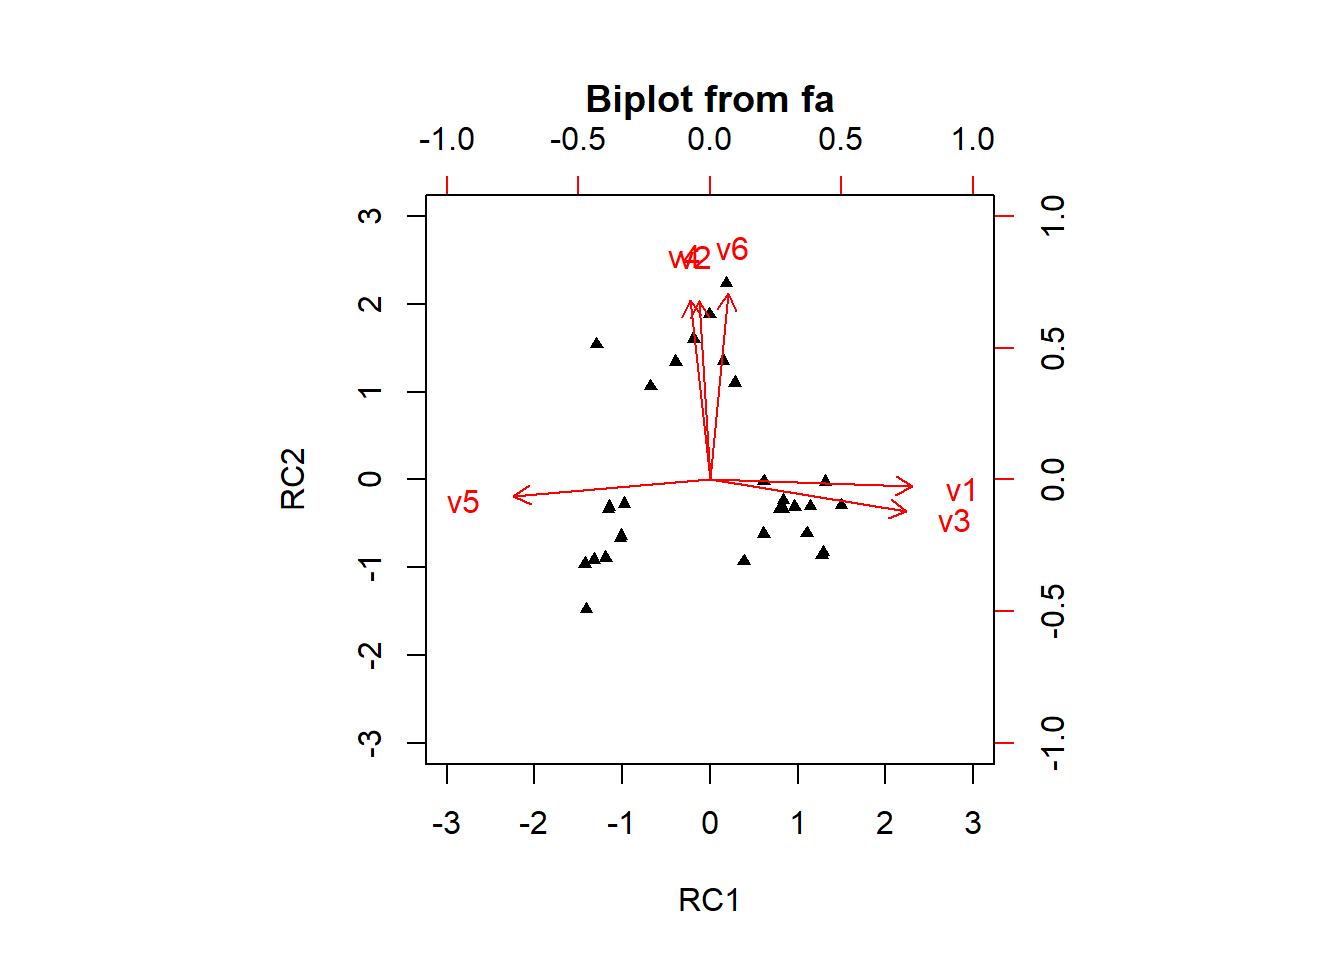
\includegraphics[width=0.8\linewidth]{index_files/figure-latex/unnamed-chunk-32-1} \end{center}

Os valores dos fatores obtidos para os 30 entrevistados encontram-se na matriz de coeficiente de escore do componente mostrada abaixo. Esta ajuda a entender como cada variável se relaciona aos escores dos componentes calculados para cada participante. Para melhor compreensão da análise dos escores dos entrevistados é importante especificar e comentar o significado de cada fator:

\textbf{Fator 1}: Fator de benefício para a saúde.

\textbf{Fator 2}: Fator de benefício social.

Analisando os escores fatoriais dos entrevistados, destacamos a seguir alguns entrevistados e seus respectivos resultados:

Entrevistado 18: 1.494934982

Este entrevistado se destacou como o primeiro colocado no ranqueamento, obtendo o maior escore ponderado, demonstrando ser bastante atento à prevenção de cáries, gengivas fortes e dentes sadios.

Entrevistado 29: 2.24121650

Este entrevistado se destacou em primeiro no segundo fator, apresentando preocupação quanto ao beneffício social da dentição: boa aparência dos dentes, hálito puro e boa aparência dos dentes.

\begin{Shaded}
\begin{Highlighting}[]
\KeywordTok{factor.scores}\NormalTok{(creme_dental_exemplo1,PCAdentevarimax, }
              \DataTypeTok{Phi =} \OtherTok{NULL}\NormalTok{, }
              \DataTypeTok{method =} \KeywordTok{c}\NormalTok{(}\StringTok{"Thurstone"}\NormalTok{, }\StringTok{"tenBerge"}\NormalTok{, }\StringTok{"Anderson"}\NormalTok{,}
                         \StringTok{"Bartlett"}\NormalTok{, }\StringTok{"Harman"}\NormalTok{,}\StringTok{"components"}\NormalTok{),}
              \DataTypeTok{rho=}\OtherTok{NULL}\NormalTok{)}
\end{Highlighting}
\end{Shaded}

\begin{verbatim}
$scores
            RC1      RC2
 [1,]  1.143442 -0.30236
 [2,] -1.164116 -0.33355
 [3,]  1.275078 -0.85487
 [4,]  0.283039  1.10542
 [5,] -1.414762 -1.47785
 [6,]  0.962546 -0.30692
 [7,]  0.386174 -0.92946
 [8,]  1.314326 -0.02535
 [9,] -1.013721 -0.63921
[10,] -1.294149  1.54533
[11,]  1.102641 -0.61320
[12,] -1.150922 -0.30735
[13,]  1.288272 -0.82867
[14,]  0.148989  1.35741
[15,] -1.326349 -0.91233
[16,]  0.789822 -0.33831
[17,]  0.608638 -0.61594
[18,]  1.494935 -0.29386
[19,] -1.026915 -0.66542
[20,] -0.394467  1.34560
[21,] -1.192011 -0.89125
[22,]  0.614235 -0.01676
[23,] -0.978198 -0.27596
[24,] -0.006907  1.88497
[25,]  0.833064 -0.23599
[26,] -0.188091  1.60734
[27,]  0.828975 -0.32987
[28,] -0.677615  1.06323
[29,]  0.182192  2.24122
[30,] -1.428148 -0.95605

$weights
          RC1       RC2
v1  0.3584504  0.009032
v2  0.0003949  0.375030
v3  0.3449550 -0.044523
v4 -0.0148037  0.376748
v5 -0.3505500 -0.057491
v6  0.0538213  0.394380

$r.scores
          RC1       RC2
RC1 1.000e+00 4.649e-16
RC2 4.441e-16 1.000e+00

$missing
 [1] 0 0 0 0 0 0 0 0 0 0 0 0 0 0 0 0 0 0 0 0 0 0 0 0 0 0 0 0 0 0

$R2
[1] NA  1
\end{verbatim}

Destacando-se os entrevistados de interesse, verifica-se:

\begin{figure}[H]

{\centering 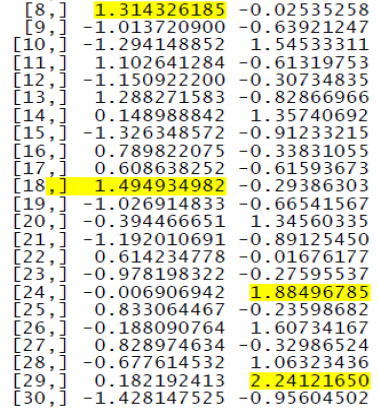
\includegraphics[width=0.8\linewidth]{anfat2} 

}

\caption{Principais resultados}\label{fig:unnamed-chunk-34}
\end{figure}

\hypertarget{analise-de-clusters}{%
\chapter{Análise de Clusters}\label{analise-de-clusters}}

\emph{Felipe Micail da Silva Smolski}

A ideia central da Análise de Cluster é a possibilidade de efetuar a classificação dos objetos em grupos, de forma que os objetos dentro do mesmo grupo sejam mais similares quanto possível e, de forma análoga, que os diversos grupos (clusters) sejam mais diferentes o possível em sua constituição (KASSAMBARA, \protect\hyperlink{ref-Kassambara2017}{2017}). Embora possa parecer semelhante ao conteúdo do capítulo anterior, as diferenças residem no fato de que a Análise Fatorial agrega variáveis e efetua os agrupamentos em base de padrões de variação (correlação) dos dados enquanto a Análise de Cluster (agrupamentos) objetiva agregar objetos (e não variáveis), fazendo a agregação baseada na distância (proximidade) (HAIR et al., \protect\hyperlink{ref-Hair2009}{2009}).

\hypertarget{k-means}{%
\section{K-Means}\label{k-means}}

O método de clusterização \emph{K-means} classifica os objetos dentro de múltiplos grupos, de forma que a variação intra-cluster seja minimizada pela soma dos quadrados das distâncias Euclidianas entre os itens e seus centroides.

\[
W(C_k)=\sum _{x_i\in C_k}(x_i-\mu _k)^2
\]
Desta forma \(x_i\) é o ponto que pertente ao cluster \(C_k\) e \(\mu _k\) representa a média do valor atribuído ao cluster \(C_k\). Cada observação (\(x_i\)) é designada a um cluster de forma que a soma dos quadrados da distância da observação em relação ao seu cluster central (\(\mu _k\)) é mínima. Ainda, para definir a variação intra-cluster é utilizadaa fórmula abaixo, sendo que deve ser tão baixa quanto o possível (KASSAMBARA, \protect\hyperlink{ref-Kassambara2017}{2017}):

\[
tot.intracluster=\sum_{k=1}^{k} W(C_k)=\sum_{k=1}^{k}\sum _{x_i\in C_k}(x_i-\mu _k)^2
\]
Como veremos adiante, deve-se selecionar o número de clusters desejado para que sejam criadas as classificações que precisar ou, executar o comando que definirá o número ótimos de clusters para a amostra carregada. O processo de seleção das variáveis, por padrão passa por (KASSAMBARA, \protect\hyperlink{ref-Kassambara2017}{2017}): (a) determinação do número de clusters; (b) selecionar randomicamente objetos para determinar os valores centrais; (c) assinar as observações pela distância Euclidiana em relação aos seus centróides; (d) efetuar atualizações calculando a nova média dos valores dentro de seu cluster definido; (e) minimizar a soma dos quadrados intra-cluster (o R utiliza 10 repetições dos passos d-e).

Vamos carregar a tradicional base de dados nativa do RStudio \texttt{mtcars}, que traz informações sobre 32 modelos de automóveis, sendo as respectivas variáveis que os descrevem:

\begin{itemize}
\tightlist
\item
  \textbf{mpg}: milhas por galão;
\item
  \textbf{cyl}: número de cilindros;
\item
  \textbf{disp}: deslocamento;
\item
  \textbf{hp}: potência;
\item
  \textbf{drat}: relação do eixo traseiro;
\item
  \textbf{wt}: peso (1.000 lbs);
\item
  \textbf{qsec}: tempo de 1/4 de milha;
\item
  \textbf{vs}: motor (0 = em forma de V; 1 = linha reta);
\item
  \textbf{am}: transmissão (0 = automático; 1 = manual);
\item
  \textbf{gear}: número de marchas na transmissão (3-4 automático; 4-5 manual);
\item
  \textbf{carb}: númerod e carburadores;
\end{itemize}

\begin{Shaded}
\begin{Highlighting}[]
\CommentTok{#Carregamento dos dados}
\KeywordTok{data}\NormalTok{(}\StringTok{"mtcars"}\NormalTok{)}
\NormalTok{df=}\KeywordTok{scale}\NormalTok{(mtcars)}
\KeywordTok{head}\NormalTok{(df, }\DataTypeTok{n=}\DecValTok{3}\NormalTok{)}
\end{Highlighting}
\end{Shaded}

\begin{verbatim}
                 mpg    cyl    disp      hp   drat      wt    qsec     vs   am
Mazda RX4     0.1509 -0.105 -0.5706 -0.5351 0.5675 -0.6104 -0.7772 -0.868 1.19
Mazda RX4 Wag 0.1509 -0.105 -0.5706 -0.5351 0.5675 -0.3498 -0.4638 -0.868 1.19
Datsun 710    0.4495 -1.225 -0.9902 -0.7830 0.4740 -0.9170  0.4260  1.116 1.19
                gear    carb
Mazda RX4     0.4236  0.7352
Mazda RX4 Wag 0.4236  0.7352
Datsun 710    0.4236 -1.1222
\end{verbatim}

A função \texttt{kmeans()} é utilizada para o cálculo, sendo que \textbf{x} representa a base de dados a ser analisada; \textbf{centers} será substituído pelo número de clusters desejados; \textbf{iter.max} representa o número de iterações para a constituição dos objetos dentro dos clusters, sendo que o padrão é 10; \textbf{nstart} é o número inicial de partições, sendo que o recomendado é superior a 1.

\texttt{kmeans(x,\ centers,\ iter.max=10,\ nstart=1)}

Para determinar automaticamente o número ótimo de clusters da classificação, antes de rodar a função \texttt{kmeans()}, é possível utilizar a função \texttt{fviz\_nbclust()} do pacote \texttt{factoextra}. Desta forma, utilizando a noção da soma dos quadrados intra cluster é possível verificar que o número ótimo de clusters para a amostra é 4. Isto porque novos clusters acima de 4 possuem baixo ganho para aumentar a diferenciação dos demais.

\begin{Shaded}
\begin{Highlighting}[]
\CommentTok{# Número ótimo de clusters}
\KeywordTok{library}\NormalTok{(factoextra)}

\KeywordTok{fviz_nbclust}\NormalTok{(df, kmeans, }\DataTypeTok{method =} \StringTok{"wss"}\NormalTok{)}\OperatorTok{+}
\StringTok{  }\KeywordTok{geom_vline}\NormalTok{(}\DataTypeTok{xintercept =} \DecValTok{4}\NormalTok{, }\DataTypeTok{linetype =} \DecValTok{2}\NormalTok{)}
\end{Highlighting}
\end{Shaded}

\begin{center}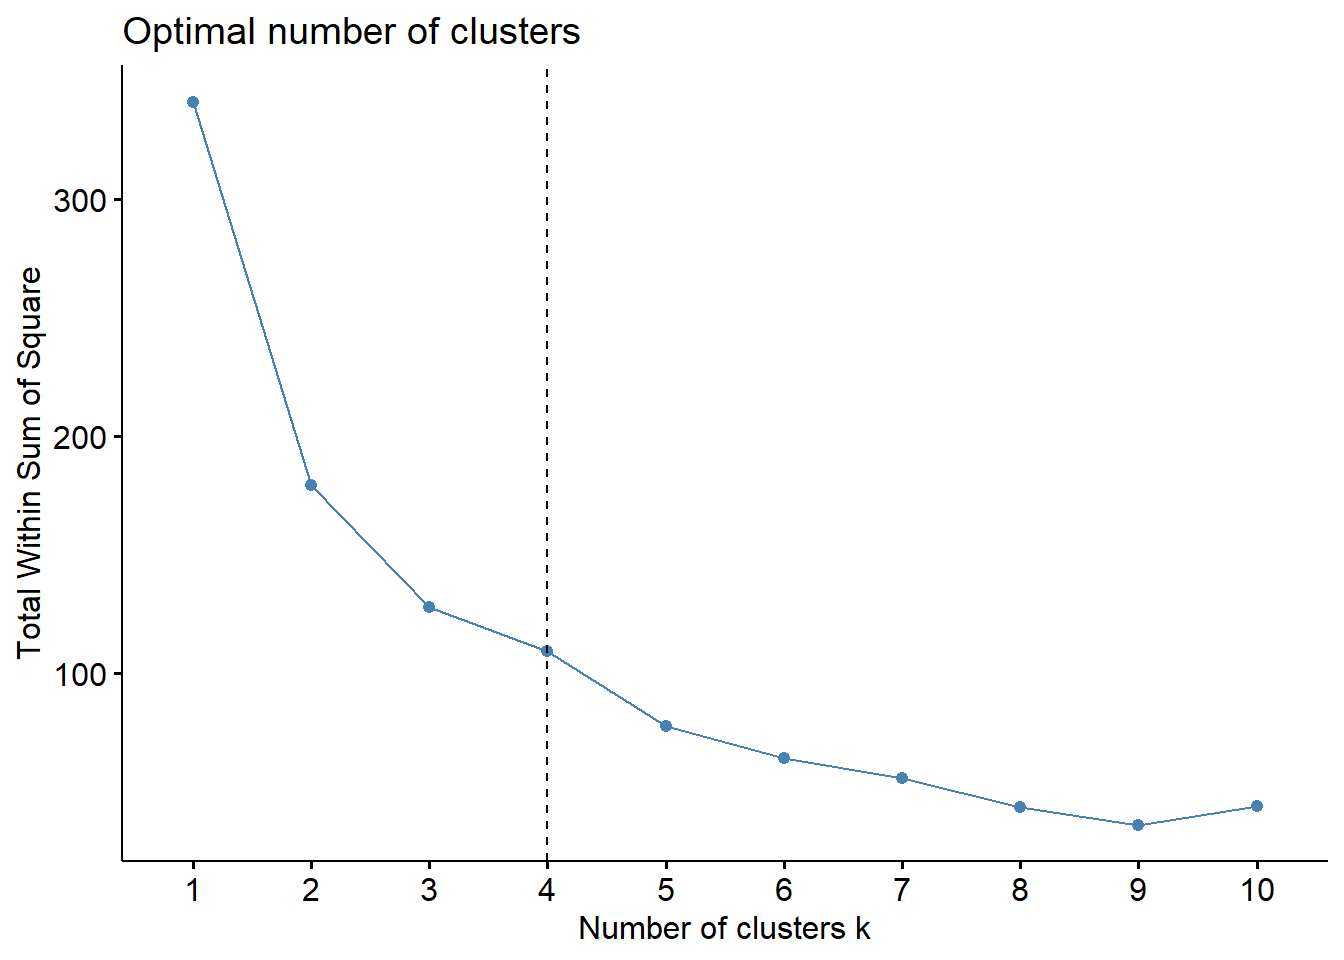
\includegraphics[width=0.8\linewidth]{index_files/figure-latex/unnamed-chunk-36-1} \end{center}

\begin{Shaded}
\begin{Highlighting}[]
\CommentTok{# Clusterização k-means}
\KeywordTok{set.seed}\NormalTok{(}\DecValTok{123}\NormalTok{)}
\NormalTok{km.res=}\KeywordTok{kmeans}\NormalTok{(df, }\DecValTok{4}\NormalTok{, }\DataTypeTok{nstart=}\DecValTok{25}\NormalTok{)}
\KeywordTok{print}\NormalTok{(km.res)}
\end{Highlighting}
\end{Shaded}

\begin{verbatim}
K-means clustering with 4 clusters of sizes 12, 8, 7, 5

Cluster means:
      mpg     cyl     disp      hp     drat       wt    qsec     vs      am
1 -0.8363  1.0149  1.02385  0.6925 -0.88975  0.90636 -0.3952 -0.868 -0.8141
2  1.3248 -1.2249 -1.10627 -0.9453  1.09821 -1.20087  0.3365  0.868  1.1899
3  0.1082 -0.5849 -0.44867 -0.6497 -0.04968 -0.02347  1.1855  1.116 -0.8141
4 -0.2639  0.3430 -0.05908  0.7601  0.44782 -0.22101 -1.2495 -0.868  1.1899
     gear    carb
1 -0.9318  0.1677
2  0.7624 -0.8126
3 -0.1573 -0.4146
4  1.2368  1.4781

Clustering vector:
          Mazda RX4       Mazda RX4 Wag          Datsun 710      Hornet 4 Drive 
                  4                   4                   2                   3 
  Hornet Sportabout             Valiant          Duster 360           Merc 240D 
                  1                   3                   1                   3 
           Merc 230            Merc 280           Merc 280C          Merc 450SE 
                  3                   3                   3                   1 
         Merc 450SL         Merc 450SLC  Cadillac Fleetwood Lincoln Continental 
                  1                   1                   1                   1 
  Chrysler Imperial            Fiat 128         Honda Civic      Toyota Corolla 
                  1                   2                   2                   2 
      Toyota Corona    Dodge Challenger         AMC Javelin          Camaro Z28 
                  3                   1                   1                   1 
   Pontiac Firebird           Fiat X1-9       Porsche 914-2        Lotus Europa 
                  1                   2                   2                   2 
     Ford Pantera L        Ferrari Dino       Maserati Bora          Volvo 142E 
                  4                   4                   4                   2 

Within cluster sum of squares by cluster:
[1] 23.08 19.04 21.29 23.40
 (between_SS / total_SS =  74.5 %)

Available components:

[1] "cluster"      "centers"      "totss"        "withinss"     "tot.withinss"
[6] "betweenss"    "size"         "iter"         "ifault"      
\end{verbatim}

\begin{Shaded}
\begin{Highlighting}[]
\KeywordTok{aggregate}\NormalTok{(mtcars, }\DataTypeTok{by=}\KeywordTok{list}\NormalTok{(}\DataTypeTok{cluster=}\NormalTok{km.res}\OperatorTok{$}\NormalTok{cluster), mean)}
\end{Highlighting}
\end{Shaded}

\begin{verbatim}
  cluster   mpg   cyl   disp     hp  drat    wt  qsec    vs am  gear  carb
1       1 15.05 8.000 357.62 194.17 3.121 4.104 17.14 0.000  0 3.000 3.083
2       2 28.07 4.000  93.61  81.88 4.184 2.042 18.45 0.875  1 4.250 1.500
3       3 20.74 5.143 175.11 102.14 3.570 3.194 19.97 1.000  0 3.571 2.143
4       4 18.50 6.800 223.40 198.80 3.836 3.001 15.62 0.000  1 4.600 5.200
\end{verbatim}

\begin{Shaded}
\begin{Highlighting}[]
\NormalTok{dd=}\KeywordTok{cbind}\NormalTok{(mtcars, }\DataTypeTok{cluster=}\NormalTok{km.res}\OperatorTok{$}\NormalTok{cluster)}
\KeywordTok{head}\NormalTok{(dd)}
\end{Highlighting}
\end{Shaded}

\begin{verbatim}
                   mpg cyl disp  hp drat    wt  qsec vs am gear carb cluster
Mazda RX4         21.0   6  160 110 3.90 2.620 16.46  0  1    4    4       4
Mazda RX4 Wag     21.0   6  160 110 3.90 2.875 17.02  0  1    4    4       4
Datsun 710        22.8   4  108  93 3.85 2.320 18.61  1  1    4    1       2
Hornet 4 Drive    21.4   6  258 110 3.08 3.215 19.44  1  0    3    1       3
Hornet Sportabout 18.7   8  360 175 3.15 3.440 17.02  0  0    3    2       1
Valiant           18.1   6  225 105 2.76 3.460 20.22  1  0    3    1       3
\end{verbatim}

\begin{Shaded}
\begin{Highlighting}[]
\NormalTok{km.res}\OperatorTok{$}\NormalTok{centers}
\end{Highlighting}
\end{Shaded}

\begin{verbatim}
      mpg     cyl     disp      hp     drat       wt    qsec     vs      am
1 -0.8363  1.0149  1.02385  0.6925 -0.88975  0.90636 -0.3952 -0.868 -0.8141
2  1.3248 -1.2249 -1.10627 -0.9453  1.09821 -1.20087  0.3365  0.868  1.1899
3  0.1082 -0.5849 -0.44867 -0.6497 -0.04968 -0.02347  1.1855  1.116 -0.8141
4 -0.2639  0.3430 -0.05908  0.7601  0.44782 -0.22101 -1.2495 -0.868  1.1899
     gear    carb
1 -0.9318  0.1677
2  0.7624 -0.8126
3 -0.1573 -0.4146
4  1.2368  1.4781
\end{verbatim}

\begin{Shaded}
\begin{Highlighting}[]
\CommentTok{# Vizualizando os clusters}

\KeywordTok{library}\NormalTok{(ggplot2)}
\KeywordTok{library}\NormalTok{(factoextra)}

\KeywordTok{fviz_cluster}\NormalTok{(km.res, }\DataTypeTok{data=}\NormalTok{dd,}
             \DataTypeTok{palette =} \KeywordTok{c}\NormalTok{(}\StringTok{"#2E9FDF"}\NormalTok{, }\StringTok{"#00AFBB"}\NormalTok{, }\StringTok{"#E7B800"}\NormalTok{, }\StringTok{"#FC4E07"}\NormalTok{),}
             \DataTypeTok{ellipse.type=}\StringTok{"euclid"}\NormalTok{,}
             \DataTypeTok{star.plot=}\OtherTok{TRUE}\NormalTok{,}
             \DataTypeTok{repel=}\OtherTok{TRUE}\NormalTok{,}
             \DataTypeTok{ggtheme=}\KeywordTok{theme_minimal}\NormalTok{()}
\NormalTok{             )}
\end{Highlighting}
\end{Shaded}

\begin{center}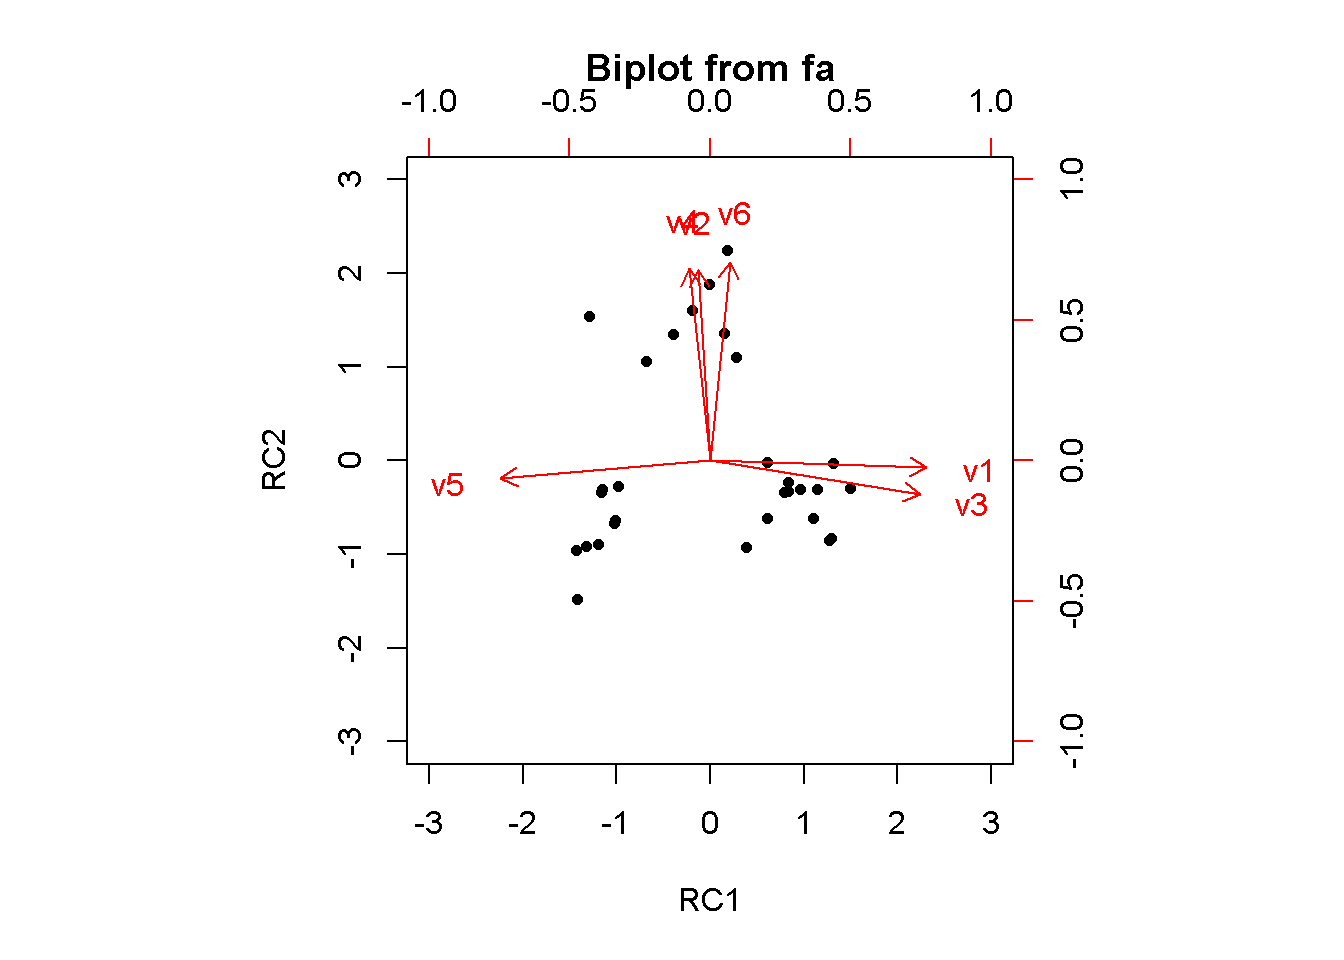
\includegraphics[width=0.8\linewidth]{index_files/figure-latex/unnamed-chunk-39-1} \end{center}

\hypertarget{agglomerative}{%
\section{Agglomerative}\label{agglomerative}}

\hypertarget{regressao-multipla}{%
\chapter{Regressão Múltipla}\label{regressao-multipla}}

\emph{Iara Denise Endruweit Battisti}

\hypertarget{modelo-geral}{%
\section{Modelo geral}\label{modelo-geral}}

Um modelo de regressão múltipla é expresso como:

\[ 
y_{i} = \beta_0+\ \beta_1x_{1i}+\beta_2x_{2i}+\dots+\beta_kx_{ki}+\varepsilon_i\ 
\]
\noindent
em que:

\begin{itemize}
\item
  \(y_{i}\): valores da variável resposta, \(i = 1, 2,..., n\) observações;
\item
  \(x\): valores das variáveis explicativas, \(k = 1, 2,..., K\) variáveis;
\item
  \(\beta_k\): parâmetros do modelo;
\item
  \(\varepsilon_i\): erro aleatório.
\end{itemize}

A equação estimada para este modelo é definida como:

\[ 
y_{i} = b_0+\ b_1x_{1i}+b_2x_{2i}+\dots+b_kx_{ki} 
\]
em que:

\begin{itemize}
\tightlist
\item
  \(b_k\): coeficientes estimados.
\end{itemize}

\hypertarget{variavel-dummy}{%
\section{Variável dummy}\label{variavel-dummy}}

Em algumas situações é necessário introduzir, como variável preditora (independente), uma variável categórica no
modelo de regressão linear simples ou múltiplo, como por exemplo, local (urbano ou rural), área (preservada ou degradada), etc, podendo ter mais que duas categorias. Essa variável terá que ser codificada, utilizando somente códigos 0 e 1, assim chamada variável dummy.

O número de variáveis dummy no modelo será sempre igual ao número de categorias da variável preditora original
menos 1. Por exemplo:

\begin{itemize}
\item
  Para a variável preditora ``local'' que assume valores - urbano ou rural, então têm-se a variável dummy
  local\_dummy assumindo 0 para rural e 1 para urbano; também, poderia ser utilizado 1 para rural e 0 para
  urbano. Uma indicação é que a categoria que assume o valor 0 seja a categoria de referência.
\item
  Para a variável preditora ``grau de escolaridade''" que assume valores -- ensino fundamental, ensino médio,
  ensino superior, então têm-se as variáveis dummy: escola1 e escola2, assim definido:
\end{itemize}

\begin{enumerate}
\def\labelenumi{\alph{enumi}.}
\tightlist
\item
  escola1=0 e escola2=0 para ensino fundamental;
\item
  escola1=1 e escola2=0 para ensino médio;
\item
  escola1=0 e escola2=1 para ensino superior.
\end{enumerate}

\textbf{Exercício}:

\begin{enumerate}
\def\labelenumi{\arabic{enumi})}
\tightlist
\item
  Utilizando o banco de dados \texttt{ARVORE2}, ajuste um modelo de regressão linear simples para predizer a altura das árvores
  em função do diâmetro. Veja essa relação no diagrama de dispersão. Interprete os resultados.
\end{enumerate}

Relembrando Modelos de Regressão Linear Simples -- Curso Básico do Software R:

\begin{itemize}
\tightlist
\item
  1.1 Ajustar a equação de regressão. Interpretá-la.
\item
  1.2 Encontrar e interpretar a significância da equação.
\item
  1.3 Encontrar e interpretar o coeficiente de determinação.
\item
  1.4 Analisar graficamente os resíduos.
\item
  1.5 Testar a normalidade dos resíduos.
\end{itemize}

Adicionalmente - Curso Avançado do Software R:

\begin{itemize}
\tightlist
\item
  1.6 Analisar pontos \emph{outliers} nos resíduos.
\end{itemize}

Para análise dos valores \emph{outliers} nos resíduos (\emph{residuals standard} e \emph{residuals studentized}), utilizam-se os seguintes comandos:

\texttt{rstudent(regressao)}

\texttt{rstandard(regressao)}

E o gráfico para verificar valores outliers nos resíduos:

\texttt{plot(rstudent(regressao))}

\texttt{plot(rstandard(regressao))}

Aqueles valores maiores que \textbar{}2\textbar{} são possíveis outliers. Incluir uma linha y =2 e y=-2, para facilitar a visualização de outliers.

\begin{itemize}
\tightlist
\item
  1.7 Analisar pontos influentes nos resíduos.
\end{itemize}

Para análise dos valores influentes, utiliza-se:

\texttt{dffits(regressao)}

Aqueles valores maiores que \texttt{2*(p/n)\^{}(1/2)} são possíveis pontos influentes. Em que, p = número de parâmetros do modelo e n = tamanho da amostra. O gráfico para detectar pontos influentes pode ser elaborado pelo comando:

\texttt{plot(dffits(regressao))}

Aqueles valores maiores, em módulo, são possíveis influentes. Incluir linhas para facilitar a visualização de pontos influentes.

Ainda, pode-se utilizar o comando \texttt{plot(regressao)} elabora diferentes gráficos para o diagnóstico do modelo.

\begin{enumerate}
\def\labelenumi{\arabic{enumi})}
\setcounter{enumi}{1}
\item
  Ajuste um segundo modelo de regressão linear simples para predizer a altura das árvores em função da espécie. Veja essa relação no diagrama de dispersão. Interprete os resultados.
\item
  Ajuste um terceiro modelo de regressão múltipla para predizer a altura das árvores em função do diâmetro e da espécie. Interprete os resultados.
\end{enumerate}

\begin{Shaded}
\begin{Highlighting}[]
\KeywordTok{library}\NormalTok{(readxl)}
\NormalTok{url <-}\StringTok{ "https://github.com/Smolski/livroavancado/raw/master/arvore2.xlsx"}
\NormalTok{destfile <-}\StringTok{ "arvore2.xlsx"}
\NormalTok{curl}\OperatorTok{::}\KeywordTok{curl_download}\NormalTok{(url, destfile)}
\NormalTok{arvore2 <-}\StringTok{ }\KeywordTok{read_excel}\NormalTok{(destfile)}
\KeywordTok{attach}\NormalTok{(arvore2)}
\KeywordTok{head}\NormalTok{(arvore2)}
\end{Highlighting}
\end{Shaded}

\begin{verbatim}
# A tibble: 6 x 4
  Nomecientifico            diametro_cm altura_m especie
  <chr>                           <dbl>    <dbl>   <dbl>
1 Sebastiania commersoniana        52.2     15.2       0
2 Sebastiania commersoniana        95       17.3       0
3 Sebastiania commersoniana        67.3     16.3       0
4 Sebastiania commersoniana        46.3     14         0
5 Sebastiania commersoniana        64.1     15         0
6 Sebastiania commersoniana       122       22         0
\end{verbatim}

\begin{Shaded}
\begin{Highlighting}[]
\NormalTok{modelom=}\KeywordTok{lm}\NormalTok{(altura_m}\OperatorTok{~}\NormalTok{diametro_cm}\OperatorTok{+}\NormalTok{especie) }
\NormalTok{modelom}
\end{Highlighting}
\end{Shaded}

\begin{verbatim}

Call:
lm(formula = altura_m ~ diametro_cm + especie)

Coefficients:
(Intercept)  diametro_cm      especie  
    12.6959       0.0571      -1.6252  
\end{verbatim}

Modelo:
\[
Y = 12,328 + 0,0576 x_1 – 1,423 x_2
\]
Ou

\[
\text{Altura} = 12,328 + 0,0576\text{diâmetro} – 1,423\text{espécie}
\]

Verificando a significância de cada coeficiente do modelo de regressão múltipla:

\begin{Shaded}
\begin{Highlighting}[]
\KeywordTok{summary}\NormalTok{(modelom)}
\end{Highlighting}
\end{Shaded}

\begin{verbatim}

Call:
lm(formula = altura_m ~ diametro_cm + especie)

Residuals:
   Min     1Q Median     3Q    Max 
-3.269 -0.766 -0.124  0.813  2.873 

Coefficients:
            Estimate Std. Error t value Pr(>|t|)    
(Intercept) 12.69592    0.38639   32.86  < 2e-16 ***
diametro_cm  0.05713    0.00445   12.84  < 2e-16 ***
especie     -1.62517    0.24459   -6.64  1.5e-09 ***
---
Signif. codes:  0 '***' 0.001 '**' 0.01 '*' 0.05 '.' 0.1 ' ' 1

Residual standard error: 1.19 on 102 degrees of freedom
Multiple R-squared:   0.7,  Adjusted R-squared:  0.694 
F-statistic:  119 on 2 and 102 DF,  p-value: <2e-16
\end{verbatim}

Verificar a significância do modelo completo.

Verificar o coeficiente de determinação do modelo.

Realizar análise dos resíduos.

\begin{itemize}
\tightlist
\item
  gráfico dos resíduos com cada variável preditora
\item
  resíduos padronizados para verificar outlier
\item
  verificar pontos infuentes
\end{itemize}

A interpretação dos termos de regressão é um pouco mais complicada. Em geral, um modelo com múltiplos preditores indica a diferença média na variável desfecho quando mudamos o valor de uma variável e mantemos a outra constante.

Nesse caso, entre árvores de mesmo diâmetro (\(x_1\)), a diferença média esperada da altura (y) para a espécie \emph{Syphoneugena reitzii} em relação a espécie \emph{Sebastiania} commersoniana é de cerca de 1,42m a menos (pois \(b_3\)=-1,42).

Da mesma forma, árvores da mesma espécie têm, em média, 0,05758m (pois \(b_2\)=0,05758) a mais a cada 1 cm de diâmetro.

Como envolvem mais variáveis, não é possível resolver o modelo inteiro num único gráfico. Como alternativa, pode-se plotar a reta para cada espécie (variável categórica).

Primeiro, os pontos são plotados. O argumento \texttt{type=\textquotesingle{}n\textquotesingle{}} indica que não é para acrescentar nenhum ponto ao gráfico.
Em seguida, os pontos são acrescentados separadamente, com a função points, a qual acrescenta pontos ao gráfico, sendo que o colchetes \texttt{{[}espécie==0{]}} seleciona somente os casos desejados.

Por fim, acrescentamos as retas de regressão para cada resposta a variável independente espécie. Usamos a função \texttt{coef} para extrair os coeficientes de interesse.

\begin{Shaded}
\begin{Highlighting}[]
\KeywordTok{plot}\NormalTok{(diametro_cm,altura_m)}
\end{Highlighting}
\end{Shaded}

\begin{center}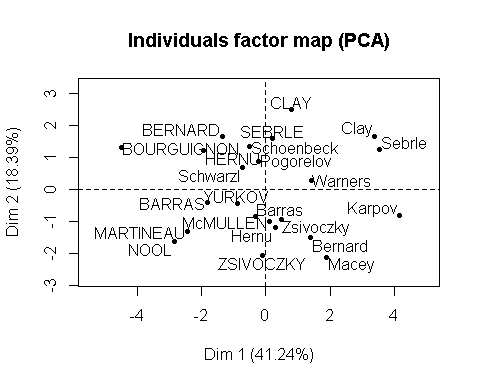
\includegraphics[width=0.8\linewidth]{index_files/figure-latex/unnamed-chunk-43-1} \end{center}

\begin{Shaded}
\begin{Highlighting}[]
\CommentTok{# Gera o gráfico sem pontos}
\KeywordTok{plot}\NormalTok{(diametro_cm,altura_m,}\DataTypeTok{type=}\StringTok{'n'}\NormalTok{) }
\CommentTok{# Acrescenta os pontos}
\KeywordTok{points}\NormalTok{(diametro_cm[especie}\OperatorTok{==}\DecValTok{0}\NormalTok{],altura_m[especie}\OperatorTok{==}\DecValTok{0}\NormalTok{],}\DataTypeTok{col=}\StringTok{'blue'}\NormalTok{)}
\KeywordTok{points}\NormalTok{(diametro_cm[especie}\OperatorTok{==}\DecValTok{1}\NormalTok{],altura_m[especie}\OperatorTok{==}\DecValTok{1}\NormalTok{],}\DataTypeTok{col=}\StringTok{'red'}\NormalTok{)}
\CommentTok{# Acrescenta as linhas}
\KeywordTok{abline}\NormalTok{(}\KeywordTok{coef}\NormalTok{(modelom)[}\DecValTok{1}\NormalTok{], }\KeywordTok{coef}\NormalTok{(modelom)[}\DecValTok{2}\NormalTok{], }\DataTypeTok{col=}\StringTok{'blue'}\NormalTok{)}
\KeywordTok{abline}\NormalTok{(}\KeywordTok{coef}\NormalTok{(modelom)[}\DecValTok{1}\NormalTok{]}\OperatorTok{+}\KeywordTok{coef}\NormalTok{(modelom)[}\DecValTok{3}\NormalTok{], }\KeywordTok{coef}\NormalTok{(modelom)[}\DecValTok{2}\NormalTok{], }\DataTypeTok{col=}\StringTok{'red'}\NormalTok{)}
\end{Highlighting}
\end{Shaded}

\begin{center}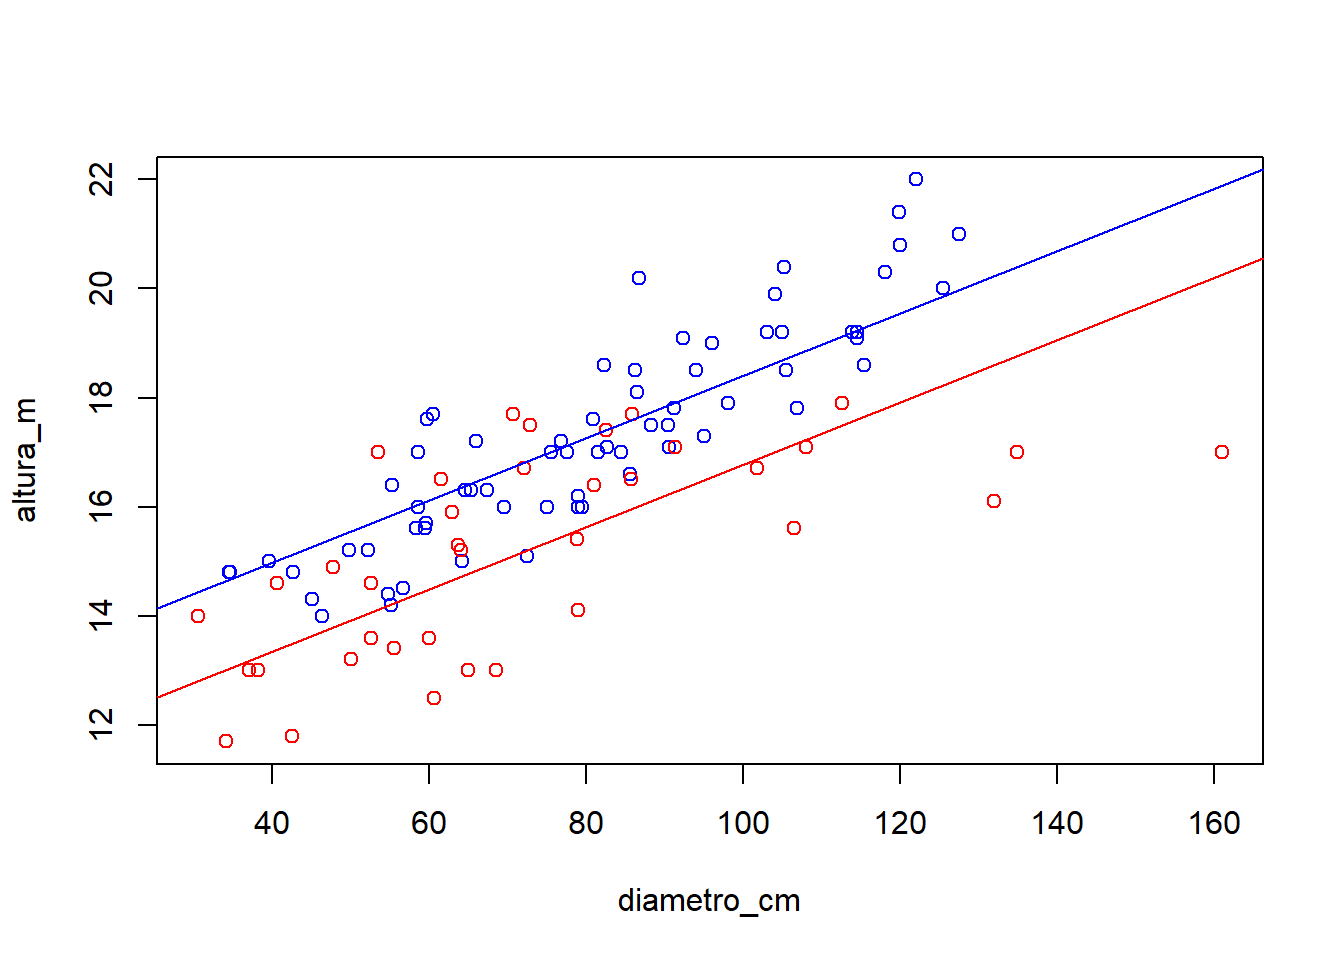
\includegraphics[width=0.8\linewidth]{index_files/figure-latex/unnamed-chunk-43-2} \end{center}

\hypertarget{interacao-entre-variaveis-preditoras}{%
\section{Interação entre variáveis preditoras}\label{interacao-entre-variaveis-preditoras}}

Quando suspeita-se que os coeficientes de inclinação podem variar entre as categorias da variável preditora então aconselha-se testar a interação entre as duas variáveis. No software R utiliza-se `:' para indicar a interação entre as duas variáveis. Se a interação for significativa (P\textless{}0,05), então conclui-se que os coeficientes de inclinação diferem entre si.

O modelo de regressão múltipla apresentando anteriormente pressupõe que a inclinação da reta de regressão é igual para os dois grupos considerados, espécie Syphoneugena reitzii e espécie Sebastiania commersoniana espécie. Se existem motivos para acreditar que a inclinação pode variar de um grupo para o outro, pode-se acrescentar um termo de interação (interação entre variáveis) (Kaszubowski, 2016).

A interação, neste caso, nada mais é do que o acréscimo de uma nova variável preditora ao modelo. Essa nova variável preditora é o produto das duas variáveis que já constam no modelo. Para acrescentar um termo de interação no R, basta utilizar dois pontos `:' entre o nome das duas variáveis para as quais se deseja criar o termo de interação.

\begin{Shaded}
\begin{Highlighting}[]
\NormalTok{modelom=}\KeywordTok{lm}\NormalTok{(}\StringTok{`}\DataTypeTok{altura_m}\StringTok{`}\OperatorTok{~}\StringTok{`}\DataTypeTok{diametro_cm}\StringTok{`}\OperatorTok{+}\NormalTok{especie}\OperatorTok{+}\StringTok{`}\DataTypeTok{diametro_cm}\StringTok{`}\OperatorTok{:}\NormalTok{especie, }\DataTypeTok{data =}\NormalTok{ arvore2)}
\NormalTok{modelom}
\end{Highlighting}
\end{Shaded}

\begin{verbatim}

Call:
lm(formula = altura_m ~ diametro_cm + especie + diametro_cm:especie, 
    data = arvore2)

Coefficients:
        (Intercept)          diametro_cm              especie  
            11.5480               0.0714               0.7863  
diametro_cm:especie  
            -0.0316  
\end{verbatim}

\begin{Shaded}
\begin{Highlighting}[]
\KeywordTok{summary}\NormalTok{(modelom)}
\end{Highlighting}
\end{Shaded}

\begin{verbatim}

Call:
lm(formula = altura_m ~ diametro_cm + especie + diametro_cm:especie, 
    data = arvore2)

Residuals:
    Min      1Q  Median      3Q     Max 
-2.2460 -0.8545  0.0632  0.7552  2.5561 

Coefficients:
                    Estimate Std. Error t value Pr(>|t|)    
(Intercept)         11.54805    0.47544   24.29  < 2e-16 ***
diametro_cm          0.07137    0.00566   12.62  < 2e-16 ***
especie              0.78630    0.68304    1.15  0.25237    
diametro_cm:especie -0.03158    0.00842   -3.75  0.00029 ***
---
Signif. codes:  0 '***' 0.001 '**' 0.01 '*' 0.05 '.' 0.1 ' ' 1

Residual standard error: 1.12 on 101 degrees of freedom
Multiple R-squared:  0.736, Adjusted R-squared:  0.728 
F-statistic:   94 on 3 and 101 DF,  p-value: <2e-16
\end{verbatim}

\begin{Shaded}
\begin{Highlighting}[]
\KeywordTok{plot}\NormalTok{(diametro_cm,altura_m,}\DataTypeTok{type=}\StringTok{'n'}\NormalTok{)}

\KeywordTok{points}\NormalTok{(diametro_cm[especie}\OperatorTok{==}\DecValTok{0}\NormalTok{],altura_m[especie}\OperatorTok{==}\DecValTok{0}\NormalTok{],}\DataTypeTok{col=}\StringTok{'blue'}\NormalTok{)}
\KeywordTok{points}\NormalTok{(diametro_cm[especie}\OperatorTok{==}\DecValTok{1}\NormalTok{],altura_m[especie}\OperatorTok{==}\DecValTok{1}\NormalTok{],}\DataTypeTok{col=}\StringTok{'red'}\NormalTok{)}

\KeywordTok{abline}\NormalTok{(}\KeywordTok{coef}\NormalTok{(modelom)[}\DecValTok{1}\NormalTok{],}\KeywordTok{coef}\NormalTok{(modelom)[}\DecValTok{2}\NormalTok{], }\DataTypeTok{col=}\StringTok{'blue'}\NormalTok{)}
\KeywordTok{abline}\NormalTok{(}\KeywordTok{coef}\NormalTok{(modelom)[}\DecValTok{1}\NormalTok{]}\OperatorTok{+}\KeywordTok{coef}\NormalTok{(modelom)[}\DecValTok{3}\NormalTok{],}\KeywordTok{coef}\NormalTok{(modelom)[}\DecValTok{2}\NormalTok{]}\OperatorTok{+}\KeywordTok{coef}\NormalTok{(modelom)[}\DecValTok{4}\NormalTok{], }\DataTypeTok{col=}\StringTok{'red'}\NormalTok{)}
\end{Highlighting}
\end{Shaded}

\begin{center}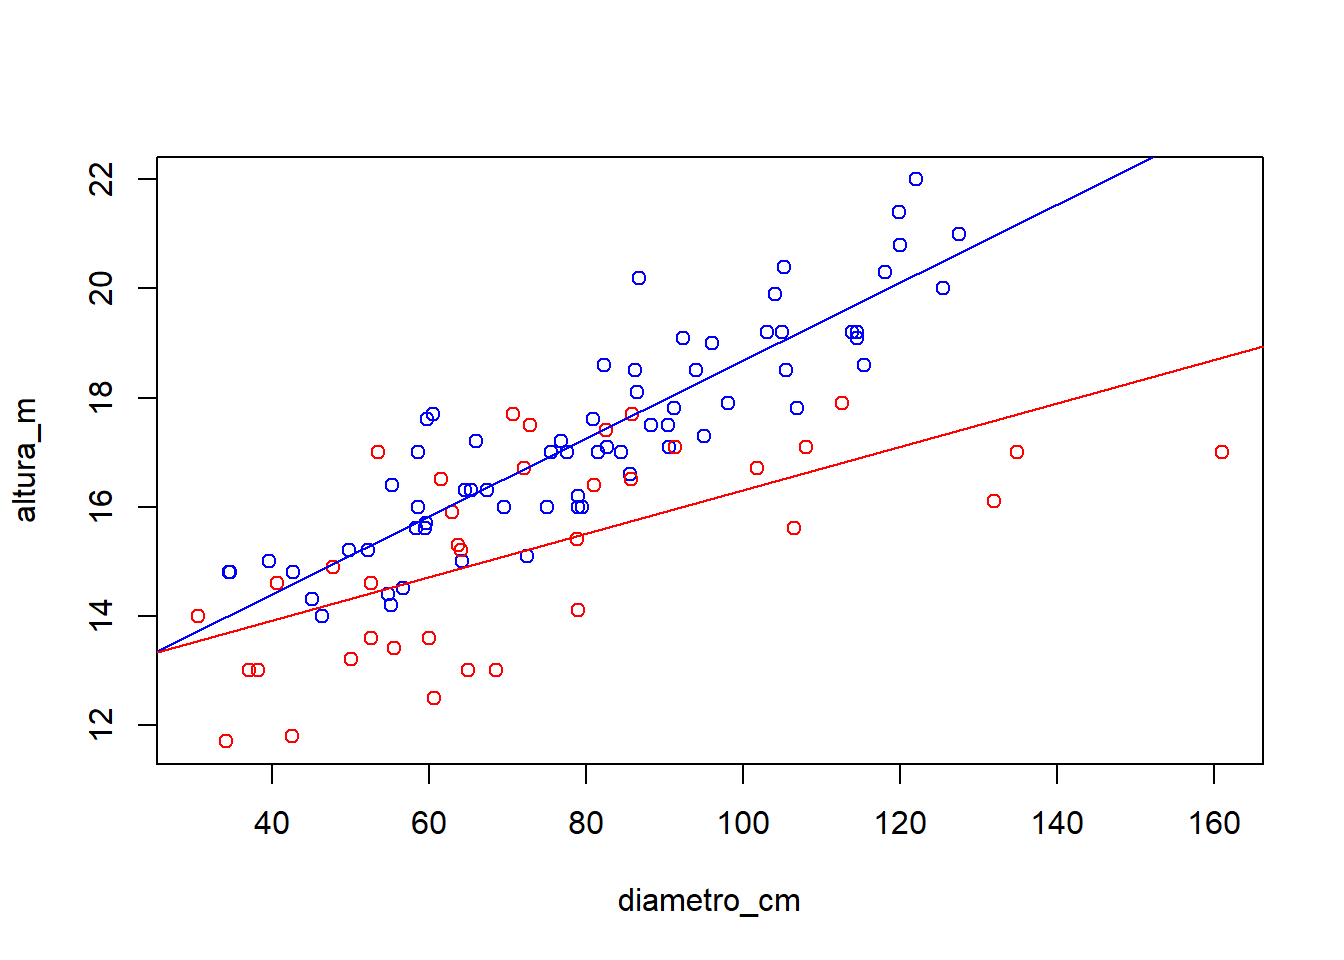
\includegraphics[width=0.8\linewidth]{index_files/figure-latex/unnamed-chunk-46-1} \end{center}

\hypertarget{metodos-selecao-de-variaveis-na-regressao-multipla}{%
\section{Métodos seleção de variáveis na regressão múltipla}\label{metodos-selecao-de-variaveis-na-regressao-multipla}}

\hypertarget{full-model-modelo-completo}{%
\subsection{Full model -- Modelo completo}\label{full-model-modelo-completo}}

Sintaxe no software R para um modelo de regressão múltipla com três variáveis preditivas:

\texttt{regressao=lm(y\textasciitilde{}x1+x2+x3)}

\texttt{summary(regressao)}

Existem três métodos de seleção de variáveis para modelos de regressão múltipla: \emph{backward}, \emph{forward} e \emph{stepwise}.

\texttt{regressao=step(lm(y\textasciitilde{}x1+x2+x3),direction\ =\ \textquotesingle{}método\textquotesingle{})}

\hypertarget{procedimento-backward}{%
\subsection{Procedimento backward}\label{procedimento-backward}}

Considera todas as variáveis inicialmente, testando posteriormente, a permanência de cada uma no modelo. Se p \(\leq\) 15\%, permanece no modelo (saiu do modelo não entra mais) (Riboldi, 2005).

Passo 1) Ajustar o modelo completo de m variáveis e obter \(SQR^{c}_{eg}\) e \(\sigma^{2}\);

Passo 2) Para cada uma das m variáveis do modelo completo do passo 1, considerar o modelo reduzido -- retirando esta variável
-- e calcular \(SQR^{r}_{eg}\) para obter o valor da estatística (slide 24);

Passo 3) Achar o mínimo dos m valores da estatística obtidos no passo 2, denotado por F\textsubscript{min};

Passo 4) Seja F\textsubscript{out} o valor da distribuição F com 1 e (n-m-1) gl;

\begin{itemize}
\item
  Se F\textsubscript{min} \textgreater{} F\textsubscript{out}: interromper o processo e optar pelo modelo completo desta etapa;
\item
  Se F\textsubscript{min} \textless{} F\textsubscript{out}: voltar ao passo 1, iniciando nova etapa em que o modelo completo tem (m-1) variáveis -- dada a
  eliminação da variável cuja estatística é igual a F\textsubscript{min}.
\end{itemize}

\hypertarget{procedimento-forward}{%
\subsection{Procedimento forward}\label{procedimento-forward}}

Inclui uma variável de cada vez, se p \(\leq\) 20\%, entra no modelo. Este método não testa a permanência da variável (entrou no modelo não sai mais) RIBOLDI (\protect\hyperlink{ref-Riboldi2005}{2005}).

Passo 1) Ajustar o modelo reduzido de m variáveis e obter \(SQR^{c}_{eg}\);

Passo 2) Para cada variável não pertencente ao modelo do passo 1, considerar o modelo completo com adição desta variável
extra e calcular \(SQR^{r}_{eg}\) e \(\sigma^{2}\) para obter o valor da estatística (slide 26);

Passo 3) Achar o máximo dos valores da estatística obtidos no passo 2, denotado por F\textsubscript{max};

Passo 4) Seja F\textsubscript{in} o valor da distribuição F com 1 e (n-m) gl;

\begin{itemize}
\item
  Se F\textsubscript{max} \textgreater{} F\textsubscript{in}: voltar ao passo 1, iniciando nova etapa em que o modelo reduzido tem (m+1) variáveis -- dada a inclusão
  da variável cuja estatística é igual a F\textsubscript{max}.
\item
  Se F\textsubscript{max} \textless{} F\textsubscript{in}: interromper o processo e optar pelo modelo reduzido desta etapa;
\end{itemize}

\hypertarget{procedimento-stepwise}{%
\subsection{Procedimento stepwise}\label{procedimento-stepwise}}

Inclui as variáveis passo-a-passo e testa a permanência (as variáveis podem entrar e sair do modelo) (Riboldi, 2005).

Passo 1) Ajustar o modelo reduzido de m variáveis e obter \(SQR^{r}_{eg}\);

Passo 2) Para cada variável não pertencente ao modelo do passo 1, considerar o modelo completo - com adição desta variável
extra - e calcular \(SQR^{c}_{eg}\) e \(\sigma^{2}\) para obter o valor da estatística (slide 26);

Passo 3) Achar o máximo dos valores da estatística obtidos no passo 2, denotado por F\textsubscript{max};

Passo 4) Seja Fin o valor da distribuição F com 1 e (n-m) gl;

\begin{itemize}
\item
  Se Fmax \textgreater{} Fin -\textgreater{} passar ao passo 5, com modelo completo composto por (m+1) variáveis -- as m variáveis do modelo do
  passo 1 e a variável cuja estatística é igual a Fmax.
\item
  Se Fmax \textless{} Fin -\textgreater{} passar ao passo 5, com modelo completo igual ao modelo do passo 1 ou encerrar o processo se no passo
  8 da etapa anterior, nenhuma variável tiver sido eliminada;
\end{itemize}

Passo 5) Ajustar o modelo completo de k variáveis -- sendo k igual a m ou (m+1), e obter \(SQR^{c}_{eg}\) e \(\sigma^{2}\);

Passo 6) Para cada uma das k variáveis do modelo completo do passo 5, considerar o modelo reduzido -- retirando esta variável -- e calcular \(SQR^{r}_{eg}\) para obter o valor da estatística;

Passo 7) Achar o mínimo dos k valores da estatística obtidos no passo 6, denotado por F\textsubscript{min};

Passo 8) Seja F\textsubscript{out} o valor da distribuição F com 1 e (n-k-1) gl;

\begin{itemize}
\item
  Se F\textsubscript{min} \textgreater{} F\textsubscript{out}: não eliminar nenhuma variável e voltar ao passo 1, iniciando nova etapa com modelo reduzido com k
  variáveis ou encerrar o processo de no passo 4 nenhuma variável tiver sido anexada;
\item
  Se Fmin \textless{} Fout: eliminar a variável cuja estatística é igual a Fmin e voltar ao passo 1 iniciando nova etapa com modelo
  reduzido com (k-1) variáveis.
\end{itemize}

\begin{figure}[H]

{\centering 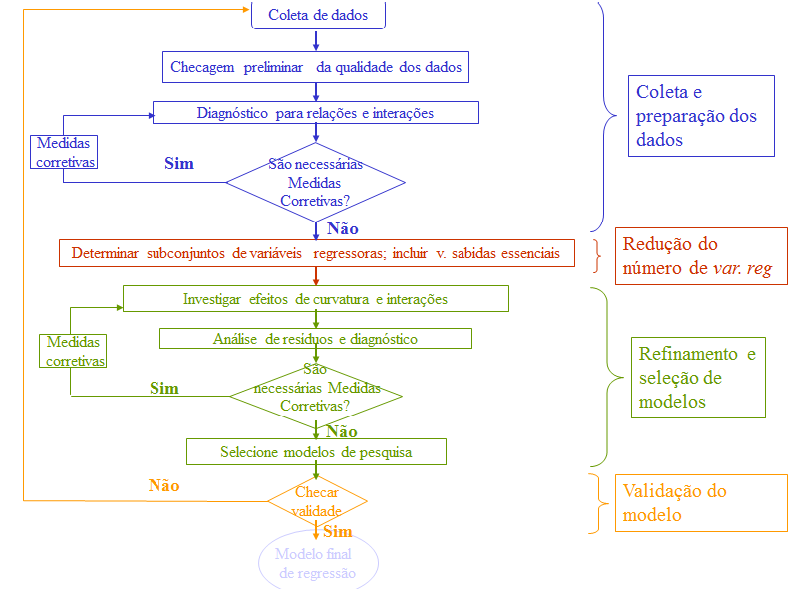
\includegraphics[width=0.8\linewidth]{regress1} 

}

\caption{Modelagem estatística}\label{fig:unnamed-chunk-47}
\end{figure}

Fonte: RIBOLDI (\protect\hyperlink{ref-Riboldi2005}{2005})

\hypertarget{roteiro-para-o-diagnostico-do-modelo-de-regressao-multipla-ajustado}{%
\section{Roteiro para o diagnóstico do modelo de regressão múltipla ajustado}\label{roteiro-para-o-diagnostico-do-modelo-de-regressao-multipla-ajustado}}

Identificação de observações destoantes para Y

\begin{itemize}
\tightlist
\item
  Resíduo studentizado externamente -- r\_student (studentized residual with currente observation deleted)
\item
  Resíduo studentizado internamente -- student (studentized residual)
\item
  Identificação de observações destoantes com base nos resíduos -- residual
\end{itemize}

Identificação de observações destoantes para X

\begin{itemize}
\tightlist
\item
  Matriz H
\item
  Alavanca (Leverage = )
\end{itemize}

Identificação de casos de influência

\begin{itemize}
\tightlist
\item
  DFFITS (standard influence of observation on predict values)
\item
  Distância de Cook (\_cookd)
\item
  DFBetas
\end{itemize}

Verificação da existência de multicolinearidade (correlação entre os X's)

\begin{itemize}
\tightlist
\item
  Matriz de correlação das variáveis
\item
  Análise de estrutura k (condition index)
\item
  Fator de inflação de variância -- VIF (variance inflation)
\item
  Teste de Durbin-Watson pra atutocorrelação
\end{itemize}

\hypertarget{regressao-com-dados-em-painel}{%
\chapter{Regressão com Dados em Painel}\label{regressao-com-dados-em-painel}}

\emph{Felipe Micail da Silva Smolski}

O modelo de regressão com dados em painel possui uma característica especial: se constitui de uma dimensão \emph{temporal} e outra \emph{espacial}. Isto porque a mesma unidade de corte transversal (família, países, etc.) é acompanhada ao longo do tempo. Por exemplo, a produção industrial mensal dos Estados brasileiros em função da taxa de juros no período de 2015-2016. Têm-se então a 624 (26x24) observações \emph{combinadas}: de cada um dos 26 Estados (exluindo o Distrito Federal) e 24 observações para os meses.

Dentre os benefícios da regressão com dados em painel (GUJARATI; PORTER, \protect\hyperlink{ref-Gujarati2011}{2011}):

\begin{itemize}
\item
  Devido à heterogeneidade da análise entre indivíduos, empresas, estados, países, etc., esta técnica pode levar em conta estas variáveis individuais específicas;
\item
  Maior informação, maior variabilidade e menor colinearidade entre variáveis, devido à combinaçãod e séries temporais e dados com corte transversal;
\item
  Dados em painel são mais adequados ao estudo da \emph{dinâmica da mudança} (emprego, renda, etc).
\item
  Detecta e mede melhor os efeitos em comparação aos estudos transversais puros ou em séries temporais puras;
\item
  Possibilidade de modelos comportamentais mais complexos;
\item
  Minimização do viés decorrente da agregação de pessoas e/ou empresas nos grandes conjuntos.
\end{itemize}

\hypertarget{carregamento-e-transformacao-dos-dados}{%
\section{Carregamento e transformação dos dados}\label{carregamento-e-transformacao-dos-dados}}

A base de dados utilizada neste exemplo (``Grunfeld'') é proveniente do pacote \texttt{AER}. É constituída da variável dependente do nível de investimento (``invest'') de diversas empresas (``firm''), bem como das variáveis explicativas de seu valor de mercado (``value'') e do valor do estoque de capital (``capital'') durante o período de 1935-1954 (20 anos). Portanto pretende-se descobrir os determinantes do valor do nível investimento das firmas durente o período.

\begin{Shaded}
\begin{Highlighting}[]
\KeywordTok{require}\NormalTok{(AER) }
\KeywordTok{data}\NormalTok{(Grunfeld, }\DataTypeTok{package=}\StringTok{"AER"}\NormalTok{)}
\end{Highlighting}
\end{Shaded}

Após carregada a base para o estudo, serão selecionadas quatro empresas (``General Electric'', ``General Motors'', ``US Steel'' e ``Westinghouse'') para fins de análise dos dados. Utiliza-se o pacote \texttt{plm} e a função \texttt{pdata.frame} para alocar a base de dados para a análise de regressão de dados em painel, uma vez que é necessário definir o atributo individual (``firm'') e temporal (``year'') das observações. Para isso utiliza-se o argumento \texttt{index}, como segue:

\begin{Shaded}
\begin{Highlighting}[]
\KeywordTok{require}\NormalTok{(plm)}

\NormalTok{Grunfeld=}\KeywordTok{subset}\NormalTok{(Grunfeld, firm }\OperatorTok\StringTok{ }\KeywordTok{c}\NormalTok{(}\StringTok{"General Electric"}\NormalTok{,}
                                      \StringTok{"General Motors"}\NormalTok{,}
                                      \StringTok{"US Steel"}\NormalTok{,}
                                      \StringTok{"Westinghouse"}\NormalTok{))}
\NormalTok{Grunfeld=}\KeywordTok{pdata.frame}\NormalTok{(Grunfeld, }\DataTypeTok{index=}\KeywordTok{c}\NormalTok{(}\StringTok{"firm"}\NormalTok{,}\StringTok{"year"}\NormalTok{))}
  
\KeywordTok{head}\NormalTok{(Grunfeld)}
\end{Highlighting}
\end{Shaded}

\begin{verbatim}
                    invest value capital           firm year
General Motors-1935  317.6  3078     2.8 General Motors 1935
General Motors-1936  391.8  4662    52.6 General Motors 1936
General Motors-1937  410.6  5387   156.9 General Motors 1937
General Motors-1938  257.7  2792   209.2 General Motors 1938
General Motors-1939  330.8  4313   203.4 General Motors 1939
General Motors-1940  461.2  4644   207.2 General Motors 1940
\end{verbatim}

\begin{Shaded}
\begin{Highlighting}[]
\KeywordTok{summary}\NormalTok{(Grunfeld)}
\end{Highlighting}
\end{Shaded}

\begin{verbatim}
     invest           value         capital                     firm   
 Min.   :  12.9   Min.   : 192   Min.   :   0.8   General Motors  :20  
 1st Qu.:  55.3   1st Qu.:1192   1st Qu.: 118.1   US Steel        :20  
 Median : 199.8   Median :1971   Median : 254.7   General Electric:20  
 Mean   : 290.9   Mean   :2229   Mean   : 357.3   Westinghouse    :20  
 3rd Qu.: 459.8   3rd Qu.:2795   3rd Qu.: 368.9                        
 Max.   :1486.7   Max.   :6242   Max.   :2226.3                        
                                                                       
      year   
 1935   : 4  
 1936   : 4  
 1937   : 4  
 1938   : 4  
 1939   : 4  
 1940   : 4  
 (Other):56  
\end{verbatim}

Nota-se que nesta base que será trabalhada os dados das empresas aparecem ``empilhados'', uma vez que a variável referente ao ano da observação (``year'') está repetida para cada observação da referida empresa (corte transversal repetido em diversos períodos de tempo). Desta forma a nossa base de dados possui igualmente 20 informações para cada empresa, se constituindo em um \emph{painel equilibrado}. Caso o número de informações para cada empresa fossem desiguais, teríamos um \emph{painel desequilibrado}.

Uma questão interessante emerge para a análise de regressão de dados em painel, em virtude da interação de variáveis individuais (``firm'') com a série temporal (``year''): a elevação da complexidade da análise. Desta forma, várias possibilidades de análise de modelos de regressão surgem, dentre elas:

\begin{enumerate}
\def\labelenumi{\alph{enumi})}
\item
  regressão considerando que o intercepto do modelo e seus coeficientes angulares são constantes ao londo do tempo e no espaço, sendo que o termo de erro capta a diferença no tempo e entre os indivíduos (POOLED);
\item
  regressão considerando que os coeficientes angulares são constantes e o intercepto varia entre os indivíduos (EFEITOS FIXOS);
\item
  regressão considerando que o intercepto assume um valor médio comum entre os indivíduos e os coeficientes angulares variam ao longo do tempo e também entre indivíduos (EFEITOS ALEATÓRIOS).
\end{enumerate}

Abaixo é demonstrada a evolução do investimento de acordo com cada empresa estudada:

\begin{Shaded}
\begin{Highlighting}[]
\KeywordTok{coplot}\NormalTok{(invest }\OperatorTok{~}\StringTok{ }\NormalTok{year}\OperatorTok{|}\NormalTok{firm, }\DataTypeTok{type=}\StringTok{"b"}\NormalTok{, }\DataTypeTok{data=}\NormalTok{Grunfeld)}
\end{Highlighting}
\end{Shaded}

\begin{center}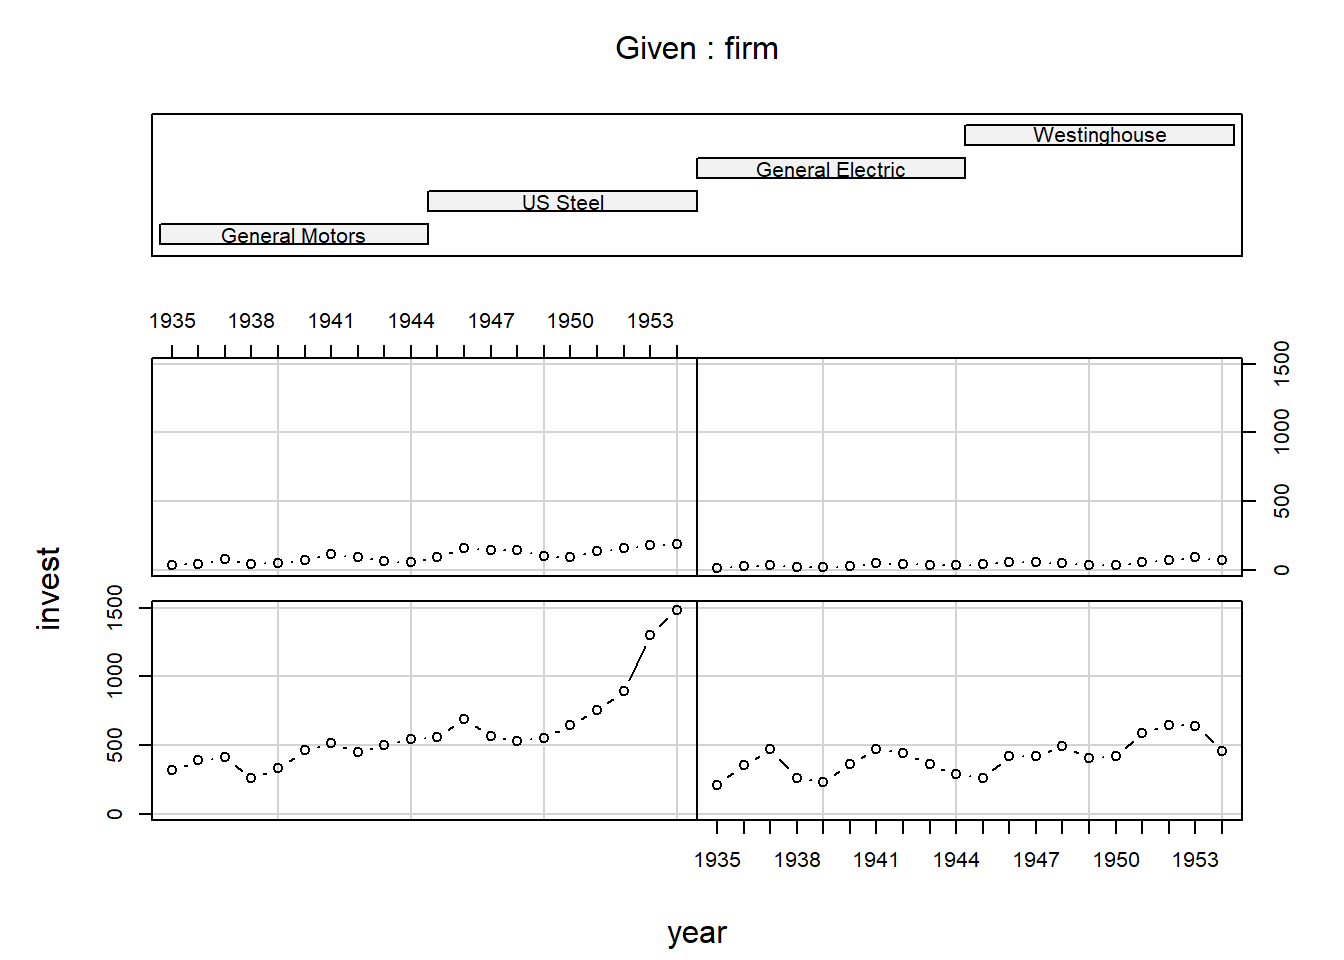
\includegraphics[width=0.8\linewidth]{index_files/figure-latex/unnamed-chunk-50-1} \end{center}

\hypertarget{modelo-pooled}{%
\section{Modelo Pooled}\label{modelo-pooled}}

Este modelo trata de ``empilhar'' todas as observações da base de dados, ignorando a estrutura de dados em painel. Desta forma, todas as observações são tratadas como não correlacionadas para os indivíduos, com erros homoscedásticos para com os indivíduos. Trata-se, portanto, da forma mais simplista e ingênua pois desconsidera as dimensões de tempo e espaço combinados, ao mesmo tempo que estima a regressão pelo método dos Mínimos Quadrados Ordinários (MQO) (GUJARATI; PORTER, \protect\hyperlink{ref-Gujarati2011}{2011}). Desta forma:

\[
 \begin{matrix}
Y_{it} = \beta_1+\beta_2X_{2it} + \beta_3X_{3it} +u_{it}\\
i=1,2,3,4\\
t=1,2,\dots,20
 \end{matrix}
\]

em que \(i\) corresponde à \(i\)-nésima unidade de corte transversal e \(t\) o \(t\)-nésimo período de tempo.

Para executar este modelo de regressão é necessário utilizar a função \texttt{plm}, juntamente com as variáveis dependente e independentes, indicando a base de dados (\texttt{data}) e o tipo da regressão (\texttt{"pooling"}).

\begin{Shaded}
\begin{Highlighting}[]
\NormalTok{reg.pooled=}\KeywordTok{plm}\NormalTok{(invest}\OperatorTok{~}\NormalTok{value}\OperatorTok{+}\NormalTok{capital, }
               \DataTypeTok{data=}\NormalTok{Grunfeld, }\DataTypeTok{model=}\StringTok{"pooling"}\NormalTok{)}
\KeywordTok{summary}\NormalTok{(reg.pooled)}
\end{Highlighting}
\end{Shaded}

\begin{verbatim}
Pooling Model

Call:
plm(formula = invest ~ value + capital, data = Grunfeld, model = "pooling")

Balanced Panel: n = 4, T = 20, N = 80

Residuals:
   Min. 1st Qu.  Median 3rd Qu.    Max. 
-319.68  -99.95    1.96   65.99  336.21 

Coefficients:
            Estimate Std. Error t-value Pr(>|t|)    
(Intercept) -62.8318    29.7254   -2.11    0.038 *  
value         0.1105     0.0138    8.02  9.2e-12 ***
capital       0.3005     0.0494    6.08  4.3e-08 ***
---
Signif. codes:  0 '***' 0.001 '**' 0.01 '*' 0.05 '.' 0.1 ' ' 1

Total Sum of Squares:    6410000
Residual Sum of Squares: 1570000
R-Squared:      0.755
Adj. R-Squared: 0.748
F-statistic: 118.424 on 2 and 77 DF, p-value: <2e-16
\end{verbatim}

A estimação da regressão \emph{pooled} averiguou alta significância estatística nas variáveis dependentes (``value'' e ``capital''), indicando sinal positivo para os coeficientes (em consonância com a literatura), bem como um valor de R\(^2\) alto. Este tipo de modelo não faz diferenciação entre a influência/diferença das empresas na variável investimento e nem se a resposta do investimento às variáveis explicativas é a mesma ao longo do tempo. Isto faz com que não se saiba se existe heterogeneidade entre as empresas. A comparação do modelo \emph{pooled} com as regressões de efeitos fixos e efeitos aleatórios, que serão estimados na sequência, servirá mostrar ao pesquisador qual é o melhor modelo dentre eles.

\hypertarget{modelo-efeitos-fixos}{%
\section{Modelo Efeitos Fixos}\label{modelo-efeitos-fixos}}

O modelo de regressão com efeitos fixos considera, como visto anteriormente, que os valores dos interceptos para cada regressão (\(\alpha_i\)) variam de acordo com o efeito de cada indivíduo (``firma'') e que os coeficientes de declividade (das variáveis independentes ``value'' e ``capital'') para cada equação são os mesmos para cada empresa, conforme equação abaixo:

\[
invest_{it} = value_{1it} + capital_{2it} + \alpha_i + \varepsilon_{it}
\]
em que \(i=1,...,4\), \(t=1,...,20\) (painel balanceado).

Desta forma, o intercepto da equação é diferente para cada empresa, mas o efeito das variáveis independentes é o mesmo sobre a variável independente. Isto indica que existe características especiais em cada empresa influenciando o investimento, como por exemplo o estilo de gestão (GUJARATI; PORTER, \protect\hyperlink{ref-Gujarati2011}{2011}).

Abaixo é montada a regressão de efeitos fixos:

\begin{Shaded}
\begin{Highlighting}[]
\NormalTok{reg.ef=}\KeywordTok{plm}\NormalTok{(invest}\OperatorTok{~}\NormalTok{value}\OperatorTok{+}\NormalTok{capital, }
           \DataTypeTok{data=}\NormalTok{Grunfeld, }\DataTypeTok{model=}\StringTok{"within"}\NormalTok{)}
\KeywordTok{summary}\NormalTok{(reg.ef)}
\end{Highlighting}
\end{Shaded}

\begin{verbatim}
Oneway (individual) effect Within Model

Call:
plm(formula = invest ~ value + capital, data = Grunfeld, model = "within")

Balanced Panel: n = 4, T = 20, N = 80

Residuals:
   Min. 1st Qu.  Median 3rd Qu.    Max. 
-184.66  -48.26    9.33   40.55  197.67 

Coefficients:
        Estimate Std. Error t-value Pr(>|t|)    
value     0.1084     0.0176    6.17  3.3e-08 ***
capital   0.3451     0.0267   12.92  < 2e-16 ***
---
Signif. codes:  0 '***' 0.001 '**' 0.01 '*' 0.05 '.' 0.1 ' ' 1

Total Sum of Squares:    2170000
Residual Sum of Squares: 422000
R-Squared:      0.806
Adj. R-Squared: 0.792
F-statistic: 153.291 on 2 and 74 DF, p-value: <2e-16
\end{verbatim}

Nota-se que o impacto do valor da empresa (``value'') e do capital (``capital'') é positivo sobre o investimento (``invest''), para todas as empresas como visto acima. Inclusive, há significância estatística
para estas variáveis. No entanto, ainda resta definir o efeito dos interceptos de cada empresa, como segue:

\begin{Shaded}
\begin{Highlighting}[]
\KeywordTok{summary}\NormalTok{(}\KeywordTok{fixef}\NormalTok{(reg.ef))}
\end{Highlighting}
\end{Shaded}

\begin{verbatim}
                 Estimate Std. Error t-value Pr(>|t|)    
General Motors      -85.5       73.5   -1.16   0.2483    
US Steel             95.0       36.7    2.59   0.0115 *  
General Electric   -246.2       35.9   -6.85  1.9e-09 ***
Westinghouse        -59.4       20.2   -2.94   0.0044 ** 
---
Signif. codes:  0 '***' 0.001 '**' 0.01 '*' 0.05 '.' 0.1 ' ' 1
\end{verbatim}

Com este resultado é possível observar que o efeito das firmas sobre o investimento parece ser diferente para cada indivíduo. Desta forma, somente a empresa US Steel consta com efeito positivo sobre o investimento. Por outo lado, a fórmula da regressão é apresentada de maneira diversa, por exemplo: \(invest = -85,515 + 0,108400value + 0,345058capital\) para a regressão considerando a General Motors; \(invest = 94.988 + 0,108400value + 0,345058capital\) considerando a firma US Steel e assim por diante.

Outra forma de visualizar a equação de efeitos fixos é utilizando a função \texttt{lm} para definir a regressão, definindo a variável ``firm'' como um fator:

\begin{Shaded}
\begin{Highlighting}[]
\KeywordTok{summary}\NormalTok{(}\KeywordTok{lm}\NormalTok{(invest}\OperatorTok{~}\NormalTok{value}\OperatorTok{+}\NormalTok{capital}\OperatorTok{+}\KeywordTok{as.factor}\NormalTok{(firm), }
           \DataTypeTok{data=}\NormalTok{Grunfeld))}
\end{Highlighting}
\end{Shaded}

\begin{verbatim}

Call:
lm(formula = invest ~ value + capital + as.factor(firm), data = Grunfeld)

Residuals:
    Min      1Q  Median      3Q     Max 
-184.66  -48.26    9.33   40.55  197.67 

Coefficients:
                                 Estimate Std. Error t value Pr(>|t|)    
(Intercept)                      -85.5153    73.4898   -1.16  0.24831    
value                              0.1084     0.0176    6.17  3.3e-08 ***
capital                            0.3451     0.0267   12.92  < 2e-16 ***
as.factor(firm)US Steel          180.5029    45.7168    3.95  0.00018 ***
as.factor(firm)General Electric -160.7122    46.6224   -3.45  0.00094 ***
as.factor(firm)Westinghouse       26.1296    64.9435    0.40  0.68859    
---
Signif. codes:  0 '***' 0.001 '**' 0.01 '*' 0.05 '.' 0.1 ' ' 1

Residual standard error: 75.5 on 74 degrees of freedom
Multiple R-squared:  0.934, Adjusted R-squared:  0.93 
F-statistic:  210 on 5 and 74 DF,  p-value: <2e-16
\end{verbatim}

Note que o intercepto definido (-85,51533) refere-se à presença da empresa General Motors. Caso seja evidenciada a presença da empresa US Steel, o valor do intercepto passa para 94,988 (= -85,51533 + 180,50295), a mesma lógica vale para as demais empresas.

\hypertarget{modelo-efeitos-aleatorios}{%
\section{Modelo Efeitos Aleatórios}\label{modelo-efeitos-aleatorios}}

No modelo de regressão com efeitos aleatórios, os efeitos individuais das firmas (``firms'') são considerados variáveis aleatórias, ao contrário do modelo visto anteriormente. Desta forma:

\[
Y_{1i}=\beta_{1i}+\beta_2X_{2it}+\beta_3X_{3it}+u_{it}
\]

onde \(\beta_{1i}\) é variável aleatória com valor médio \(\beta_1\), e o intercepto para a empresa individual é dado por (GUJARATI; PORTER, \protect\hyperlink{ref-Gujarati2011}{2011}):

\[
\beta_{1i} = \beta_{1}+\varepsilon_{i} \quad i=1,2,\dots,N
\]
em que \(\varepsilon_{i}\) é um termo de erro de média zero e variânvia \(\sigma^{2}_{\varepsilon}\). Assim, as empresas possuem um valor médio para o intercepto (=\(\beta_1\)), sendo que as diferenças refletem o termo de erro \(\varepsilon_i\). Obtêm-se:

\[
 \begin{matrix}
Y_{it}=\beta_1+\beta_2X_{2it}+\beta_3X_{3it}+ w_{it}\\
w_{it}=\varepsilon_i+u_{it}
 \end{matrix}
\]

O erro composto \(w_{it}\) é formado por \(\varepsilon_i\) - elemento de corte transversal dos indivíduos e \(u_{it}\), que é o elemento da série temporal e do corte transversal (GUJARATI; PORTER, \protect\hyperlink{ref-Gujarati2011}{2011}). Desta forma, assume-se que os erros individuais não estão correlacionados entre si e também não estão correlacionados entre aquelas unidades de corte transversal e das séries temporais.

A montagem deste tipo de regressão é feita através da função \texttt{plm}, incluindo como modelo ``random'' e como método ``walhus'', como segue:

\begin{Shaded}
\begin{Highlighting}[]
\NormalTok{reg.ea=}\KeywordTok{plm}\NormalTok{(invest}\OperatorTok{~}\NormalTok{value}\OperatorTok{+}\NormalTok{capital,}
           \DataTypeTok{data=}\NormalTok{Grunfeld, }\DataTypeTok{model=}\StringTok{"random"}\NormalTok{, }
           \DataTypeTok{random.method =} \StringTok{"walhus"}\NormalTok{)}
\KeywordTok{summary}\NormalTok{(reg.ea)}
\end{Highlighting}
\end{Shaded}

\begin{verbatim}
Oneway (individual) effect Random Effect Model 
   (Wallace-Hussain's transformation)

Call:
plm(formula = invest ~ value + capital, data = Grunfeld, model = "random", 
    random.method = "walhus")

Balanced Panel: n = 4, T = 20, N = 80

Effects:
                  var std.dev share
idiosyncratic  5786.5    76.1  0.29
individual    13872.6   117.8  0.71
theta: 0.857

Residuals:
   Min. 1st Qu.  Median 3rd Qu.    Max. 
-193.89  -46.17    1.35   41.98  198.11 

Coefficients:
            Estimate Std. Error t-value Pr(>|t|)    
(Intercept) -72.6322    68.9083   -1.05      0.3    
value         0.1079     0.0167    6.48    8e-09 ***
capital       0.3443     0.0269   12.81   <2e-16 ***
---
Signif. codes:  0 '***' 0.001 '**' 0.01 '*' 0.05 '.' 0.1 ' ' 1

Total Sum of Squares:    2260000
Residual Sum of Squares: 446000
R-Squared:      0.802
Adj. R-Squared: 0.797
F-statistic: 156.365 on 2 and 77 DF, p-value: <2e-16
\end{verbatim}

Os resultados corroboram com a direção dos sinais para as variáveis dependentes ``value'' e ``capital'', ambos positivos. Por outro lado, os resultados do modelo de efeitos aleatórios trazem os valores sobre a variância dos erros, primeiramente voltado ao componente de corte transversal (específico dos indivíduos) denominado \texttt{individual}, e outro fator idissiossincrático, o qual varia com o tempo e também com o corte transversal, denominado \texttt{idiosyncratic}.

\hypertarget{comparacao-e-escolha-dos-modelos}{%
\section{Comparação e escolha dos modelos}\label{comparacao-e-escolha-dos-modelos}}

Após a evidenciação dos modelos de regressão dos tipos agrupado (pooled), de efeitos fixos e de efeitos aleatórios, é preciso efetuar os testes para definir qual é o melhor modelo e que por consequência deverá ser considerado.

\begin{itemize}
\tightlist
\item
  \textbf{Modelo Pooled x Modelo de Efeitos Fixos}
\end{itemize}

Inicialmente compara-se o modelo Pooled com a regressão de Efeitos Fixos (\emph{within}). Para isto utiliza-se o Teste F ou teste F de Chow. A hipótese nula é de que há igualdade nos interceptos e nas inclinações para todos os indivíduos, caracterizando o modelo de dados agrupados (pooled). A função utilizada é \texttt{pFtest()} do pacote \texttt{plm}.

\begin{Shaded}
\begin{Highlighting}[]
\KeywordTok{require}\NormalTok{(plm)}
\KeywordTok{pFtest}\NormalTok{(reg.ef,reg.pooled)}
\end{Highlighting}
\end{Shaded}

\begin{verbatim}

    F test for individual effects

data:  invest ~ value + capital
F = 67, df1 = 3, df2 = 74, p-value <2e-16
alternative hypothesis: significant effects
\end{verbatim}

Como o valor \emph{p} é inferior a 0,05, o modelo de Efeitos Fixos é melhor do que o modelo Pooled.

\begin{itemize}
\tightlist
\item
  \textbf{Modelo Pooled x Modelo de Efeitos Aleatórios}
\end{itemize}

O teste desenvolvido por Breusch e Pagan (\protect\hyperlink{ref-breusch1980}{1980}) compara as estimativas entre os modelos, verificando se \(\sigma^{2}_{\alpha} = 0\), sendo que:

\[
 \begin{matrix}
H_{0}: \sigma^{2}_{\alpha} = 0 \\
H_{1}: \sigma^{2}_{\alpha} \neq 0
 \end{matrix}
\]

Desta forma, a aceitação da hipótese nula implica que o modelo de dados agrupados (pooled) é preferível. A função \texttt{plmtest} efetua este teste:

\begin{Shaded}
\begin{Highlighting}[]
\KeywordTok{plmtest}\NormalTok{(reg.pooled, }\DataTypeTok{type=}\StringTok{"bp"}\NormalTok{)}
\end{Highlighting}
\end{Shaded}

\begin{verbatim}

    Lagrange Multiplier Test - (Breusch-Pagan) for balanced panels

data:  invest ~ value + capital
chisq = 380, df = 1, p-value <2e-16
alternative hypothesis: significant effects
\end{verbatim}

Como o \emph{p} valor foi inferior a 0,05 o modelo de Efeitos Aleatórios é superior ao modelo Pooled.

\begin{itemize}
\tightlist
\item
  \textbf{Modelo Efeitos Fixos x Modelo de Efeitos Aleatórios}
\end{itemize}

O teste de Hausmann (HAUSMAN, \protect\hyperlink{ref-hausman1978}{1978}) efetua a especificação dos modelos de Efeito Fixo e de Efeitos Aleatórios, sendo que se o teste rejeitar a hipótese nula, o modelo de Efeitos Fixos é o mais adequado.

\[
 \begin{matrix}
H_0: \alpha_{i} \text{não são correlacionados com } X_{it} \\
H_1: \alpha_{i} \text{são correlacionados com } X_{it}
 \end{matrix}
\]
A função a ser utilizada para este teste é \texttt{phtest}:

\begin{Shaded}
\begin{Highlighting}[]
\KeywordTok{phtest}\NormalTok{(reg.ef,reg.ea)}
\end{Highlighting}
\end{Shaded}

\begin{verbatim}

    Hausman Test

data:  invest ~ value + capital
chisq = 0.075, df = 2, p-value = 1
alternative hypothesis: one model is inconsistent
\end{verbatim}

Como o valor \emph{p} foi superior a 0,05 o modelo de Efeitos Aleatórios foi considerado superior ao modelo de Efeitos Fixos.

\hypertarget{alguns-testes-para-os-modelos}{%
\section{Alguns testes para os modelos}\label{alguns-testes-para-os-modelos}}

\hypertarget{testando-dependencia-transversal-cross-sectional}{%
\subsection{\texorpdfstring{Testando dependência transversal (\emph{cross-sectional})}{Testando dependência transversal (cross-sectional)}}\label{testando-dependencia-transversal-cross-sectional}}

A dependência \emph{cross-sectional} se apresenta em panieis com longas séries de tempo. A hipótese nula é de que os resíduos através dos indivíduos não estão correlacionados. Como resultado, nossa regressão aceita a hipótese nula do teste de Pesaran (\protect\hyperlink{ref-pesaran2015}{2015}):

\begin{Shaded}
\begin{Highlighting}[]
\KeywordTok{pcdtest}\NormalTok{(reg.ea, }\DataTypeTok{test=}\StringTok{"cd"}\NormalTok{)}
\end{Highlighting}
\end{Shaded}

\begin{verbatim}

    Pesaran CD test for cross-sectional dependence in panels

data:  invest ~ value + capital
z = 0.31, p-value = 0.8
alternative hypothesis: cross-sectional dependence
\end{verbatim}

\hypertarget{normalidade-dos-residuos}{%
\subsection{Normalidade dos resíduos}\label{normalidade-dos-residuos}}

Segue o já conhecido teste para verificar a normalidade dos resíduos. Como resultado, foi aprovada a hipótese nula (H\(_0\)) de normalidade nos resíduos da regressão.

\begin{Shaded}
\begin{Highlighting}[]
\KeywordTok{shapiro.test}\NormalTok{(reg.ea}\OperatorTok{$}\NormalTok{residuals)}
\end{Highlighting}
\end{Shaded}

\begin{verbatim}

    Shapiro-Wilk normality test

data:  reg.ea$residuals
W = 0.99, p-value = 0.9
\end{verbatim}

\hypertarget{homocedasticidade-dos-residuos}{%
\subsection{Homocedasticidade dos resíduos}\label{homocedasticidade-dos-residuos}}

Abaixo o teste para homocedasticidade (variância constante) dos resíduos de Breusch-Pagan (\protect\hyperlink{ref-breusch1979}{1979}):

\begin{Shaded}
\begin{Highlighting}[]
\KeywordTok{library}\NormalTok{(lmtest)}
\KeywordTok{bptest}\NormalTok{(reg.ea)}
\end{Highlighting}
\end{Shaded}

\begin{verbatim}

    studentized Breusch-Pagan test

data:  reg.ea
BP = 7.6, df = 2, p-value = 0.02
\end{verbatim}

Como a hipótese nula é a de que não há homocedasticidade nos resíduos e o \emph{p-value} foi inferior a 0,05, há problemas nos resíduos da regressão, portanto as veriáveis apresentam problemas de heterocedasticidade. Algumas soluções são possíveis, como a transformação das variáveis.

\hypertarget{testando-correlacao-serial}{%
\subsection{Testando correlação serial}\label{testando-correlacao-serial}}

A hipótese nula do teste de correlação serial do teste Breusch-Godfrey/Wooldridge (BREUSCH, \protect\hyperlink{ref-breusch1978}{1978}) é a de que não se encontra esta característica na série. Abaixo o resultado do teste, sendo que aprovou a hipótese nula, ou seja, não há problemas de correlação serial nos dados, pois o \emph{p-value} é superior a 0,05.

\begin{Shaded}
\begin{Highlighting}[]
\CommentTok{# teste Breusch-Godfrey/Wooldridge - EFEITOS ALEATÓRIOS}
\KeywordTok{pbgtest}\NormalTok{(reg.ea) }
\end{Highlighting}
\end{Shaded}

\begin{verbatim}

    Breusch-Godfrey/Wooldridge test for serial correlation in panel models

data:  invest ~ value + capital
chisq = 26, df = 20, p-value = 0.2
alternative hypothesis: serial correlation in idiosyncratic errors
\end{verbatim}

\hypertarget{teste-para-efeitos-individuais-ou-de-tempo}{%
\subsection{Teste para efeitos individuais ou de tempo}\label{teste-para-efeitos-individuais-ou-de-tempo}}

Pode ser efetuado o teste para verificar a presença de efeitos não observados de tempo ou individuais nos modelos de dados em painel (WOOLDRIDGE, \protect\hyperlink{ref-wooldridge2010}{2010}). A hipótse nula é a não correlação entre os erros do mesmo grupo. Observa-se que para o efeito tempo (``time'') há aceitação da hipótese alternativa, mostrando a correlação entre erros, ao contrário do efeito individual:

\begin{Shaded}
\begin{Highlighting}[]
\CommentTok{# teste Wooldridge - POOLED}
\KeywordTok{pwtest}\NormalTok{(reg.pooled) }
\end{Highlighting}
\end{Shaded}

\begin{verbatim}

    Wooldridge's test for unobserved individual effects

data:  formula
z = 1.4, p-value = 0.2
alternative hypothesis: unobserved effect
\end{verbatim}

\begin{Shaded}
\begin{Highlighting}[]
\KeywordTok{pwtest}\NormalTok{(reg.pooled, }\DataTypeTok{effect =} \StringTok{"time"}\NormalTok{) }
\end{Highlighting}
\end{Shaded}

\begin{verbatim}

    Wooldridge's test for unobserved time effects

data:  formula
z = -3.2, p-value = 0.001
alternative hypothesis: unobserved effect
\end{verbatim}

\hypertarget{testando-raizes-unitarias}{%
\subsection{Testando raízes unitárias}\label{testando-raizes-unitarias}}

O teste de Dickey-Fuller prova se a série é estocástica, sendo que a hipótese nula é de que a série possui raiz unitária (não-estacionaridade). Abaixo o resultado do teste, sendo que observou-se que a série é não estacionária, ou seja, tem problemas para a regressão pois o \emph{p-value} aprovou a hipótese nula. Desta forma, algumas saídas são possíveis, como a transformação da série ou mesmo a utilização da primeira diferença da série.

\begin{Shaded}
\begin{Highlighting}[]
\KeywordTok{require}\NormalTok{(tseries)}
\end{Highlighting}
\end{Shaded}

\begin{verbatim}
Carregando pacotes exigidos: tseries
\end{verbatim}

\begin{Shaded}
\begin{Highlighting}[]
\KeywordTok{adf.test}\NormalTok{(Grunfeld}\OperatorTok{$}\NormalTok{invest, }\DataTypeTok{k=}\DecValTok{2}\NormalTok{)}
\end{Highlighting}
\end{Shaded}

\begin{verbatim}

    Augmented Dickey-Fuller Test

data:  Grunfeld$invest
Dickey-Fuller = -3.4, Lag order = 2, p-value = 0.07
alternative hypothesis: stationary
\end{verbatim}

\hypertarget{regressao-logistica}{%
\chapter{Regressão Logística}\label{regressao-logistica}}

A técnica de regressão logística é uma ferramenta estatística utilizada nas análises preditivas. O interesse em mensurar a probabilidade de um evento ocorrer é extremamente relevante em diversas áreas, como por exemplo em Marketing, Propaganda e Internet, na Aplicação da Lei e Detecção de Fraude, na Assistência Médica, com relação aos Riscos Financeiros e Seguros ou mesmo estudando a Força de Trabalho. É imprescindível elevar o conhecimento sobre quais clientes possuem maior propensão à responder o contato de marketing, quais transações serão fraudulentas, quais e-mails são \emph{spam}, quem efetivamente fará o pagamento de uma obrigação ou mesmo qual criminoso reincidirá.\footnote{Para mais exemplos como estes sobre análises preditivas, ver SIEGEL (\protect\hyperlink{ref-Siegel2017}{2017}).}

\hypertarget{o-modelo}{%
\section{O modelo}\label{o-modelo}}

O modelo de regressão logística é utilizado quando a variável dependente é binária, categórica ordenada ou mesmo categórica desordenada (quando não há relação hierárquica entre elas). Abaixo exemplificam-se algumas perguntas que podem levar a estes três tipos de variáveis.

\begin{longtable}[]{@{}lll@{}}
\caption{\label{tab:logtip}Tipos de variáveis}\tabularnewline
\toprule
\endhead
\begin{minipage}[t]{0.30\columnwidth}\raggedright
\textbf{Variável dependente binária:}\strut
\end{minipage} & \begin{minipage}[t]{0.30\columnwidth}\raggedright
Você votou na última eleição?\strut
\end{minipage} & \begin{minipage}[t]{0.30\columnwidth}\raggedright
0 - Não; 1 - Sim\strut
\end{minipage}\tabularnewline
\begin{minipage}[t]{0.30\columnwidth}\raggedright
\textbf{Variável dependente categórica ordenada:}\strut
\end{minipage} & \begin{minipage}[t]{0.30\columnwidth}\raggedright
Você concorda ou desconcorda com o presidente?\strut
\end{minipage} & \begin{minipage}[t]{0.30\columnwidth}\raggedright
1 - Disconcordo; 2 - Neutro; 3 - Concordo\strut
\end{minipage}\tabularnewline
\begin{minipage}[t]{0.30\columnwidth}\raggedright
\textbf{Variável dependente categórica não ordenada:}\strut
\end{minipage} & \begin{minipage}[t]{0.30\columnwidth}\raggedright
Se as eleições fossem hoje, em que partido você votaria?\strut
\end{minipage} & \begin{minipage}[t]{0.30\columnwidth}\raggedright
1 - Democratas; 2 - Qualquer um; 3 - Republicanos\strut
\end{minipage}\tabularnewline
\bottomrule
\end{longtable}

Fonte: Adaptado de TORRES-REYNA (\protect\hyperlink{ref-Torres-Reyna2014}{2014}).

Nota-se primeiramente que em sendo somente a variável dependente \textbf{binária} (0 e 1), é detectada a presença ou não de determinada característica da variável a ser estudada pelo pesquisador. Outros exemplos abrangem a qualificação dos indivíduos estaudados em sendo do sexo feminino (1) ou do sexo masculino (0), se a empresa analisada está inadimplente (1) ou não (0) no mês de referência, etc. Por outro lado, quando a variável dependente é \textbf{categórica ordenada}, há uma hierarquia determinada entre as variáveis resposta (neste caso entre Disconcordo, Neutro e Concordo). No terceiro exemplo, a variável resposta é \textbf{categórica não ordenada} não possuindo nenhuma relação de ordem entre elas (Democratas, Qualquer um, Republicanos).

A regressão logística a ser estudada neste capítulo será com a variável resposta dependente binária, portanto, tratando os grupos de interesse (variável dependente) com valores de 0 e 1. Sua funcionalidade se ocupa de prever a probabilidade de uma observação estar no grupo igual a 1 (``eventos''), em relação ao grupo igual a zero (``não eventos'').

A previsão da variável dependente depende dos coeficientes logísticos e das variáveis independentes escolhidas ao modelo, lembrando que os valores sempre estarão entre 0 e 1. Convenciona-se que valores de probabilidade acima de 0,50 sejam classificados como pertencendo ao grupo de ``eventos'', o que pode distinguir a os resultados preditos e avaliando a precisão preditiva. Utiliza-se a razão de desigualdades - a razão entre as probabilidades dos dois resultados ou eventos: Prob\(_{i}/\)(1-Prob\(_{i}\)).

Para a estimação dos coeficientes das variáveis independentes, são utilizados o valor logit ou a razão de desigualdades (HAIR et al., \protect\hyperlink{ref-Hair2009}{2009}):

\[
Logit_i=ln\left (\frac{prob_{eventos}}{1-prob_{eventos}}  \right )=b_0+b_1X_1+\ldots+b_nX_n
\]

ou

\[
Logit_i=\left (\frac{prob_{eventos}}{1-prob_{eventos}}  \right )=e^{b_0+b_1X_1+\ldots+b_nX_n}
\]

Algumas características importantes da regressão logística: a análise é semelhante à regressão linear simples/múltipla (possui a relação entre a variável dependente e a(s) variável(is) independente(s)); possui testes estatísticos diretos, incorporando variáveis métricas e não-métricas, com efeitos não-lineares; é menos afetada pela não satisfação de normalidade dos dados (pois o termo de erro da variável discreta segue a distribuição binomial) e; foi elaborada para que seja prevista a probabilidade de determinado evento ocorrer (HAIR et al., \protect\hyperlink{ref-Hair2009}{2009}).

A regressão logística utiliza a \textbf{curva logística} para assim representar a relação entre a variável dependente e as independentes. Os valores previstos portanto permanecem entre 0 e 1, sendo definidos pelos coeficientes estimados. A Figura \ref{fig:curvalog}a demonstra a relação da curva logistica geral, enquanto a Figura \ref{fig:curvalog}b mostra uma relação pobremente ajustada dos dados reais e a Figura \ref{fig:curvalog}c demonstra um bom ajuste na relação entre as variáveis.

\begin{figure}[H]

{\centering 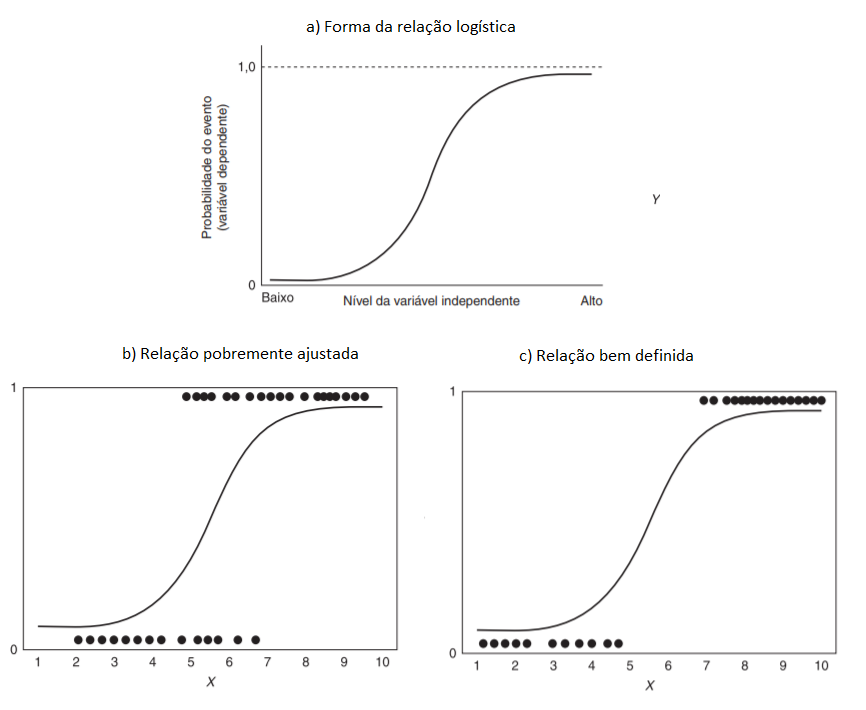
\includegraphics[width=0.8\linewidth]{curvalog} 

}

\caption{Curva logística}\label{fig:curvalog}
\end{figure}

Fonte: Adaptado de HAIR et al. (\protect\hyperlink{ref-Hair2009}{2009}).

A estimação dos coeficientes da regressão logística, ao contrário da regressão múltipla que utiliza o método dos mínimos quadrados, é efetuada pelo uso da \textbf{máxima verossimilhança}. Esta, por sua vez, busca encontrar as estimativas mais prováveis dos coeficientes e maximizar a probabilidade de que um evento ocorra. A qualidade do ajuste do modelo é avaliada pelo ``pseudo'' R\(^2\) e pelo exame da precisão preditiva (matriz de confusão).

O valor de verossimilhança é parecido com o procedimento das somas dos quadrados da regressão múltipla, estimando o quão bem o procedimento de máxima verossimilhança se ajusta ao modelo. O ajuste da estimação do modelo dá-se pelo valor -2 vezes o logaritmo da verossimilhança (-2LL), sendo que quando menor este valor, melhor o modelo (HAIR et al., \protect\hyperlink{ref-Hair2009}{2009}).

Para otimizar o tempo do estudante, é recomendada a instalação prévia dos pacotes no RStudio a serem utilizados neste capítulo. Segue abaixo o comando a ser efetuado no console do RStudio:

\texttt{install.packages(c("readr","mfx","caret","pRoc",}

\texttt{"ResourceSelection","modEvA","foreign","stargazer"))}

\hypertarget{regressao-logistica-simples}{%
\section{Regressão Logística Simples}\label{regressao-logistica-simples}}

Este primeiro exemplo tratará da regressão logística simples, portanto, utilizando somente uma variável independente, neste caso numérica. Os dados são originados do livro de HOSMER; LEMESCHOW (\protect\hyperlink{ref-Hosmer2000}{2000}), tratando-se de uma amostra com 100 pessoas. A variável dependente é a ocorrência ou não (1 ou 0) de doença coronária cardíaca (CHD), associando-se com a idade (AGE) dos indivíduos, criando assim um modelo de regressão logística.

\begin{Shaded}
\begin{Highlighting}[]
\KeywordTok{require}\NormalTok{(readr)}
\end{Highlighting}
\end{Shaded}

\begin{verbatim}
Carregando pacotes exigidos: readr
\end{verbatim}

\begin{Shaded}
\begin{Highlighting}[]
\NormalTok{chd <-}\StringTok{ }\KeywordTok{read_delim}\NormalTok{(}\StringTok{"https://github.com/Smolski/livroavancado/raw/master/cdh.csv"}\NormalTok{, }
    \StringTok{";"}\NormalTok{, }\DataTypeTok{escape_double =} \OtherTok{FALSE}\NormalTok{, }\DataTypeTok{col_types =} \KeywordTok{cols}\NormalTok{(}\DataTypeTok{CHD =} \KeywordTok{col_factor}\NormalTok{(}\DataTypeTok{levels =} \KeywordTok{c}\NormalTok{())), }
    \DataTypeTok{trim_ws =} \OtherTok{TRUE}\NormalTok{)}

\KeywordTok{summary}\NormalTok{(chd)}
\end{Highlighting}
\end{Shaded}

\begin{verbatim}
      AGE            AGRP      CHD   
 Min.   :20.0   Min.   :1.00   0:57  
 1st Qu.:34.8   1st Qu.:2.75   1:43  
 Median :44.0   Median :4.00         
 Mean   :44.4   Mean   :4.48         
 3rd Qu.:55.0   3rd Qu.:7.00         
 Max.   :69.0   Max.   :8.00         
\end{verbatim}

Observa-se na figura abaixo a dispersão dos ``eventos'' e dos ``nao-eventos'' da CHD relacionando-se com a variável idade (AGE).

\begin{Shaded}
\begin{Highlighting}[]
\KeywordTok{require}\NormalTok{(ggplot2)}

\KeywordTok{ggplot}\NormalTok{(chd, }\KeywordTok{aes}\NormalTok{(}\DataTypeTok{x=}\NormalTok{AGE, }\DataTypeTok{y=}\NormalTok{CHD)) }\OperatorTok{+}\StringTok{ }
\StringTok{  }\KeywordTok{geom_point}\NormalTok{() }\OperatorTok{+}\StringTok{ }
\StringTok{  }\KeywordTok{stat_smooth}\NormalTok{(}\DataTypeTok{method=}\StringTok{"glm"}\NormalTok{, }\DataTypeTok{method.args=}\KeywordTok{list}\NormalTok{(}\DataTypeTok{family=}\StringTok{"binomial"}\NormalTok{), }\DataTypeTok{se=}\OtherTok{FALSE}\NormalTok{)}
\end{Highlighting}
\end{Shaded}

\begin{figure}[H]

{\centering 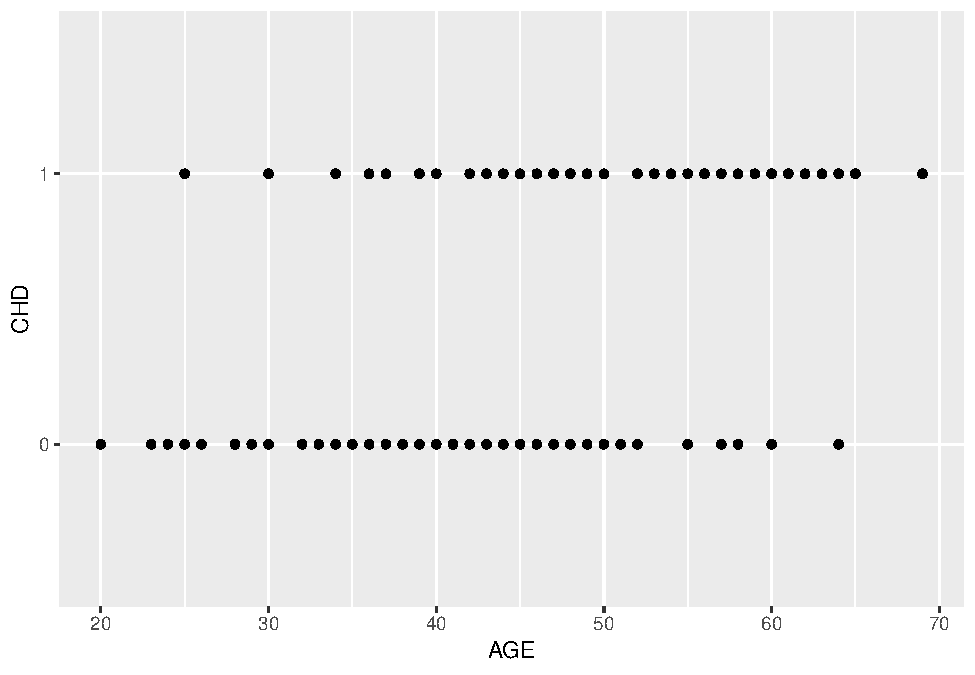
\includegraphics[width=0.8\linewidth]{index_files/figure-latex/dispev-1} 

}

\caption{Dispersão de evendos e não-eventos}\label{fig:dispev}
\end{figure}

Monta-se então o modelo de regressão logística com a variável dependente CHD e a variável independente AGE. Abaixo é demonstrada a descrição da equação utilizando o comando \texttt{summary()} para o modelo m1 com a sintaxe básica:

\texttt{glm(Y\textasciitilde{}modelo,\ family=binomial(link="logit"))}

Assim é obtida a função de ligação estimada do modelo:

\[
ln\left (\frac{prob_{CHD}}{1-prob_{CHD}}  \right ) = - 5,309 + 0,1109AGE
\]

\begin{Shaded}
\begin{Highlighting}[]
\NormalTok{m1=}\KeywordTok{glm}\NormalTok{(CHD}\OperatorTok{~}\NormalTok{AGE, }\DataTypeTok{family =} \KeywordTok{binomial}\NormalTok{(}\DataTypeTok{link=}\StringTok{"logit"}\NormalTok{), }\DataTypeTok{data =}\NormalTok{ chd)}
\KeywordTok{summary}\NormalTok{(m1)}
\end{Highlighting}
\end{Shaded}

\begin{verbatim}

Call:
glm(formula = CHD ~ AGE, family = binomial(link = "logit"), data = chd)

Deviance Residuals: 
   Min      1Q  Median      3Q     Max  
-1.972  -0.846  -0.458   0.825   2.286  

Coefficients:
            Estimate Std. Error z value Pr(>|z|)    
(Intercept)  -5.3095     1.1337   -4.68  2.8e-06 ***
AGE           0.1109     0.0241    4.61  4.0e-06 ***
---
Signif. codes:  0 '***' 0.001 '**' 0.01 '*' 0.05 '.' 0.1 ' ' 1

(Dispersion parameter for binomial family taken to be 1)

    Null deviance: 136.66  on 99  degrees of freedom
Residual deviance: 107.35  on 98  degrees of freedom
AIC: 111.4

Number of Fisher Scoring iterations: 4
\end{verbatim}

Se observa o intercepto com o valor de -5,309, sendo que para a análise aqui proposta da relação entre CHD e AGE não obtém-se um significado prático para este resultado. No entanto, a variável de interesse é idade, que no modelo de regressão obteve o coeficiente de 0,1109. Pelo fato de ser positivo informa que quando a idade (AGE) se eleva, elevam-se as chances de ocorrência de CHD. De igual forma, nota-se que há significância estatística a \(p=0,001\) na utilização da variável AGE para o modelo, mostrando que possui importância ao modelo de regressão proposto.

Por fim, o modelo é utilizado para construção da predição de todos os valores das idades de todos os indivíduos desta amostra. Para isto, será criada um novo objeto contendo somente a variável dependente do modelo (AGE) e em sequida, é criada nova coluna constando os valores preditos. Assim, pode ser plotado um gráfico completo com todas as probabilidades desta base de dados:

\begin{Shaded}
\begin{Highlighting}[]
\CommentTok{# Filtrando a idade dos indivíduos}
\NormalTok{IDADE<-chd[,}\DecValTok{1}\NormalTok{]  }

\CommentTok{# Criando campo de predição para cada idade dos indivíduos }
\NormalTok{chd}\OperatorTok{$}\NormalTok{PRED=}\KeywordTok{predict}\NormalTok{(m1, }\DataTypeTok{newdata=}\NormalTok{IDADE, }\DataTypeTok{type=}\StringTok{"response"}\NormalTok{)}

\CommentTok{# Plotando a probabilidade predita pelo modelo}
\KeywordTok{require}\NormalTok{(ggplot2)}
\KeywordTok{ggplot}\NormalTok{(chd, }\KeywordTok{aes}\NormalTok{(}\DataTypeTok{x=}\NormalTok{AGE, }\DataTypeTok{y=}\NormalTok{PRED)) }\OperatorTok{+}\StringTok{ }
\StringTok{  }\KeywordTok{geom_point}\NormalTok{()}
\end{Highlighting}
\end{Shaded}

\begin{figure}[H]

{\centering 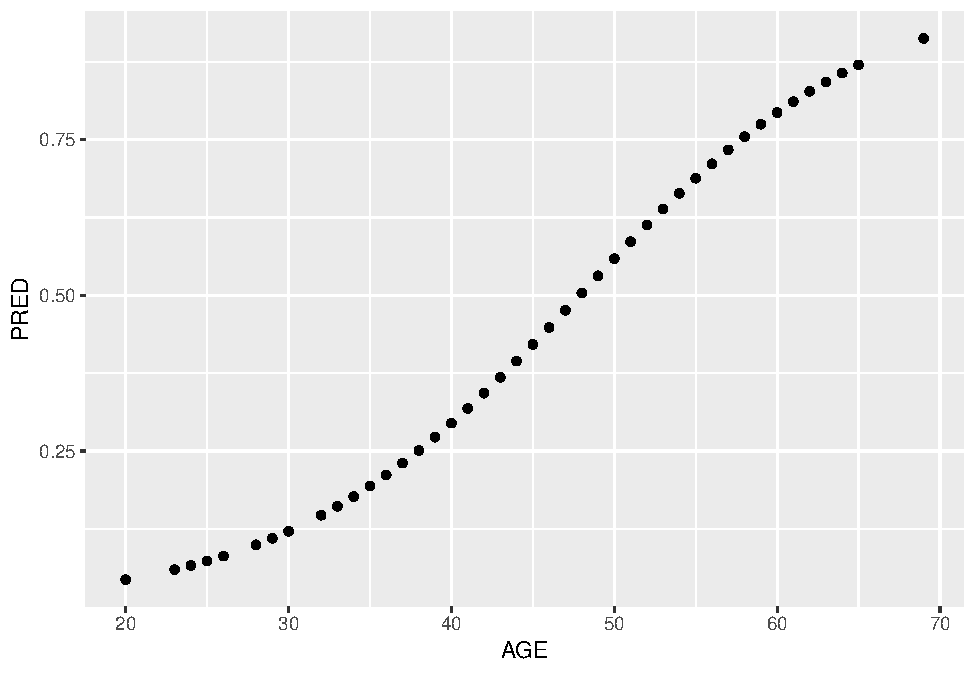
\includegraphics[width=0.8\linewidth]{index_files/figure-latex/distrpred-1} 

}

\caption{Distribuição das probabilidades preditas}\label{fig:distrpred}
\end{figure}

\hypertarget{estimando-a-razao-de-chances}{%
\subsection{Estimando a Razão de Chances}\label{estimando-a-razao-de-chances}}

O modelo de regressão logística, porém, traz os resultados dos estimadores na forma logarítma, ou seja, o log das chances da variável idade no modelo é 0,1109. No entanto, para uma interpretação mais enriquecida da relação da idade com o CHD é necessária a transformação deste coeficiente, ou seja, que seja efetuada a exponenciação da(s) variavel(eis) da regressão. Assim, obtém-se a razão das chances (OR - Odds Ratio em inglês) para as variáveis independentes.

Uma maneira prática de se obter a razão de chances no RStudio é utilizando o pacote \(mfx\). Novamente o intercepto não nos interessa nesta análise mas sim a variável AGE. Como demonstrado abaixo, o resultado da razão de chances da variável AGE foi de 1,1173, o que pode assim ser interpretado: para cada variação unitária na idade (AGE), as chances de ocorrência de CHD aumentam 1,1173 vezes. Dito de outra forma, para cada variação unitária em AGE, aumentam-se 11,73\% ((1,1173-1)*100) as chances da ocorrência de CHD.

\begin{Shaded}
\begin{Highlighting}[]
\KeywordTok{require}\NormalTok{(mfx)}
\KeywordTok{logitor}\NormalTok{(CHD}\OperatorTok{~}\NormalTok{AGE,}\DataTypeTok{data =}\NormalTok{ chd)}
\end{Highlighting}
\end{Shaded}

\begin{verbatim}
Call:
logitor(formula = CHD ~ AGE, data = chd)

Odds Ratio:
    OddsRatio Std. Err.    z P>|z|    
AGE    1.1173    0.0269 4.61 4e-06 ***
---
Signif. codes:  0 '***' 0.001 '**' 0.01 '*' 0.05 '.' 0.1 ' ' 1
\end{verbatim}

\hypertarget{determinando-o-intervalo-de-confianca}{%
\subsection{Determinando o Intervalo de Confiança}\label{determinando-o-intervalo-de-confianca}}

A determinação do intervalo de confiança do modelo proposto é relevante para que seja analizada a estimativa do intervalo de predição do coeficiente da variável independente, a um nível de confiança de 95\%. Desta forma, em 95\% dos casos, o parâmetro dos coeficientes estará dentro deste intervalo.

De forma prática é possível determinar os intervalos de confiança com o comando \texttt{confint()} commo observado abaixo, sendo que o coeficiente AGE toma o valor de 1,1173, podendo variar de 1,0692 a 1,1758.

\begin{Shaded}
\begin{Highlighting}[]
\KeywordTok{exp}\NormalTok{(}\KeywordTok{cbind}\NormalTok{(}\DataTypeTok{OR=}\KeywordTok{coef}\NormalTok{(m1), }\KeywordTok{confint}\NormalTok{(m1)))}
\end{Highlighting}
\end{Shaded}

\begin{verbatim}
                  OR     2.5 %  97.5 %
(Intercept) 0.004945 0.0004413 0.03892
AGE         1.117307 1.0692223 1.17587
\end{verbatim}

\hypertarget{predicao-de-probabilidades}{%
\subsection{Predição de Probabilidades}\label{predicao-de-probabilidades}}

A partir dos coeficientes do modelo de regressão logística é possível, portanto, efetuar a predição da variável categórica CHD, ou seja, saber a chance de ocorrer CHD com relação à uma determinada idade (AGE). No exemplo abaixo, primeiramente utilizamos a idade média das observações (44,38 anos), criando assim um novo data.frame chamado media. Para utilizar o valor da idade média na função de regressão obtida (\(m1\)), utiliza-se a função \texttt{predict()}, de acordo com valor da média encontrada (data.frame media). O resultado mostra que para a idade média da amostra, 44,38 anos, há uma probabilidade de 40,44\% na ocorrência da doença CHD. Esta ferramenta permite também a comparação pelo pesquisador das diferentes probabilidades entre as diversas idades (variável AGE).

\begin{Shaded}
\begin{Highlighting}[]
\NormalTok{media =}\StringTok{ }\KeywordTok{data.frame}\NormalTok{(}\DataTypeTok{AGE=}\KeywordTok{mean}\NormalTok{(chd}\OperatorTok{$}\NormalTok{AGE))}
\NormalTok{media}
\end{Highlighting}
\end{Shaded}

\begin{verbatim}
    AGE
1 44.38
\end{verbatim}

\begin{Shaded}
\begin{Highlighting}[]
\NormalTok{media}\OperatorTok{$}\NormalTok{pred.prob =}\StringTok{ }\KeywordTok{predict}\NormalTok{(m1, }\DataTypeTok{newdata=}\NormalTok{media, }\DataTypeTok{type=}\StringTok{"response"}\NormalTok{)}
\NormalTok{media}
\end{Highlighting}
\end{Shaded}

\begin{verbatim}
    AGE pred.prob
1 44.38    0.4045
\end{verbatim}

\hypertarget{matriz-de-confusao}{%
\subsection{Matriz de Confusão}\label{matriz-de-confusao}}

Uma maneira prática de qualificar o ajuste do modelo de regressão logística é pela projeção do modelo na tabela de classificação (ou Matriz de Confusão). Para isto, precisa-se criar uma tabela com o resultado da classificação cruzada da variável resposta, de acordo com uma variável dicotômica em que os valores se derivam das probabilidades logísticas estimadas na regressão (HOSMER; LEMESCHOW, \protect\hyperlink{ref-Hosmer2000}{2000}). No entanto, é preciso definir uma regra de predição, que dirá se houve acerto ou não da probabilidade estimada com os valores reais, pois as probabilidades variam de 0 a 1 enquanto os valores reais binários possuem valores fixos de 0 ``ou'' 1.

É intuitivo supor que se as probabilidades aproximam-se de 1 o indivíduo estimado pode ser classificado como \(\hat Y_i=1\), bem como de forma contrária, se o modelo estimar probabilidades perto de 0, classificá-la como \(\hat Y_i=0\). Mas qual nível utilizar? Para resolver este problema, é preciso em primeiro lugar determinar um ponto de corte para classificar a estimação como 0 ou 1. Usualmente na literatura se utiliza o valor de 0,5 mas dependendo do estudo proposto pode não ser limitado a este nível (HOSMER; LEMESCHOW, \protect\hyperlink{ref-Hosmer2000}{2000}).

Após determinado o ponto de corte, é importante avaliar o poder de discriminação do modelo, pelo seu desempenho portanto em classificar os ``eventos'' dos ``não eventos''. Cria-se a Matriz de Confusão (vide Tabela \ref{tab:matriz}) com as observações de Verdadeiro Positivo (VP), Falso Positivo (FP), Falso Negativo (FN) e Verdadeiro Negativo (VN) e em seguida determinam-se alguns parâmetros numéricos, a serem descritos abaixo:

\textbf{Precisão}: representa a proporção das predições corretas do modelo sobre o total:

\[
ACC=\frac{VP+VN}{P+N}
\]

onde \(P\) representa o total de ``eventos'' positivos (Y=1) e N é o total de ``não eventos'' (Y=0, ou negativo).

\textbf{Sensibilidade}: representa a proporção de verdadeiros positivos, ou seja, a capacidade do modelo em avaliar o evento como \(\hat Y=1\) (estimado) dado que ele é evento real \(Y=1\):

\[
SENS=\frac{VP}{FN}
\]

\textbf{Especificidade}: a proporção apresentada dos verdadeiros negativos, ou seja, o poder de predição do modelo em avaliar como ``não evento'' \(\hat Y=0\) sendo que ele não é evento \(Y=0\):

\[
SENS=\frac{VN}{VN+FP}
\]

\textbf{Verdadeiro Preditivo Positivo}: se caracteriza como proporção de verdadeiros positivos com relação ao total de predições positivas, ou seja, se o evento é real \(Y=1\) dada a classificação do modelo \(\hat Y=1\):

\[
VPP=\frac{VPP}{VN+FP}
\]

\textbf{Verdadeiro Preditivo Negativo}: se caracteriza pela proporção de verdadeiros negativos comparando-se com o total de predições negativas, ou seja, o indivíduo não ser evento \(Y=0\) dada classificação do modelo como ``não evento'' \(\hat Y=0\):

\[
VPN=\frac{VN}{VN+FN}
\]

\begin{longtable}[]{@{}llll@{}}
\caption{\label{tab:matriz}Matriz de confusão.}\tabularnewline
\toprule
\begin{minipage}[b]{0.25\columnwidth}\raggedright
\strut
\end{minipage} & \begin{minipage}[b]{0.15\columnwidth}\raggedright
\strut
\end{minipage} & \begin{minipage}[b]{0.25\columnwidth}\raggedright
\textbf{Valor Observado}\strut
\end{minipage} & \begin{minipage}[b]{0.14\columnwidth}\raggedright
\strut
\end{minipage}\tabularnewline
\midrule
\endfirsthead
\toprule
\begin{minipage}[b]{0.25\columnwidth}\raggedright
\strut
\end{minipage} & \begin{minipage}[b]{0.15\columnwidth}\raggedright
\strut
\end{minipage} & \begin{minipage}[b]{0.25\columnwidth}\raggedright
\textbf{Valor Observado}\strut
\end{minipage} & \begin{minipage}[b]{0.14\columnwidth}\raggedright
\strut
\end{minipage}\tabularnewline
\midrule
\endhead
\begin{minipage}[t]{0.25\columnwidth}\raggedright
\strut
\end{minipage} & \begin{minipage}[t]{0.15\columnwidth}\raggedright
\strut
\end{minipage} & \begin{minipage}[t]{0.25\columnwidth}\raggedright
\(Y=1\)\strut
\end{minipage} & \begin{minipage}[t]{0.14\columnwidth}\raggedright
\(Y=0\)\strut
\end{minipage}\tabularnewline
\begin{minipage}[t]{0.25\columnwidth}\raggedright
\textbf{Valor Estimado}\strut
\end{minipage} & \begin{minipage}[t]{0.15\columnwidth}\raggedright
\(\hat Y\)=1\strut
\end{minipage} & \begin{minipage}[t]{0.25\columnwidth}\raggedright
VP\strut
\end{minipage} & \begin{minipage}[t]{0.14\columnwidth}\raggedright
FP\strut
\end{minipage}\tabularnewline
\begin{minipage}[t]{0.25\columnwidth}\raggedright
\strut
\end{minipage} & \begin{minipage}[t]{0.15\columnwidth}\raggedright
\(\hat Y\)=0\strut
\end{minipage} & \begin{minipage}[t]{0.25\columnwidth}\raggedright
FN\strut
\end{minipage} & \begin{minipage}[t]{0.14\columnwidth}\raggedright
VN\strut
\end{minipage}\tabularnewline
\bottomrule
\end{longtable}

Fonte: Adaptado de FAWCETT (\protect\hyperlink{ref-Fawcett2006}{2006}).

\begin{Shaded}
\begin{Highlighting}[]
\KeywordTok{require}\NormalTok{(caret)}
\end{Highlighting}
\end{Shaded}

\begin{verbatim}
Carregando pacotes exigidos: caret
\end{verbatim}

\begin{verbatim}
Carregando pacotes exigidos: lattice
\end{verbatim}

\begin{verbatim}

Attaching package: 'caret'
\end{verbatim}

\begin{verbatim}
The following object is masked from 'package:survival':

    cluster
\end{verbatim}

\begin{Shaded}
\begin{Highlighting}[]
\NormalTok{chd}\OperatorTok{$}\NormalTok{pdata <-}\StringTok{ }\KeywordTok{as.factor}\NormalTok{(}
    \KeywordTok{ifelse}\NormalTok{(}
        \KeywordTok{predict}\NormalTok{(m1, }
                \DataTypeTok{newdata =}\NormalTok{ chd, }
                \DataTypeTok{type =} \StringTok{"response"}\NormalTok{)}
        \OperatorTok{>}\FloatTok{0.5}\NormalTok{,}\StringTok{"1"}\NormalTok{,}\StringTok{"0"}\NormalTok{))}

\KeywordTok{confusionMatrix}\NormalTok{(chd}\OperatorTok{$}\NormalTok{pdata, chd}\OperatorTok{$}\NormalTok{CHD, }\DataTypeTok{positive=}\StringTok{"1"}\NormalTok{)}
\end{Highlighting}
\end{Shaded}

\begin{verbatim}
Confusion Matrix and Statistics

          Reference
Prediction  0  1
         0 45 14
         1 12 29
                                        
               Accuracy : 0.74          
                 95% CI : (0.643, 0.823)
    No Information Rate : 0.57          
    P-Value [Acc > NIR] : 0.000319      
                                        
                  Kappa : 0.467         
 Mcnemar's Test P-Value : 0.844519      
                                        
            Sensitivity : 0.674         
            Specificity : 0.789         
         Pos Pred Value : 0.707         
         Neg Pred Value : 0.763         
             Prevalence : 0.430         
         Detection Rate : 0.290         
   Detection Prevalence : 0.410         
      Balanced Accuracy : 0.732         
                                        
       'Positive' Class : 1             
                                        
\end{verbatim}

A matriz de confusão retoma uma excelente acurácia total do modelo em 74\%, sendo que o modelo consegue acertos de 70,7\% na predição de valores positivos ou dos ``eventos'' (29/41) e 76,3\% na predição de valores negativos ou os ``não eventos'' (45/59).

\hypertarget{curva-roc}{%
\subsection{Curva ROC}\label{curva-roc}}

A Curva ROC (Receiver Operating Characteristic Curve) associada ao modelo logístico mensura a capacidade de predição do modelo proposto, através das predições da sensibilidade e da especificidade. Segundo FAWCETT (\protect\hyperlink{ref-Fawcett2006}{2006}) esta técnica serve para visualizar, organizar e classificar o modelo com base na performance preditiva.

A curva ROC é produzida bi-dimensionalmente como mostra a Figura \ref{fig:curvaroc}a, pela obtenção da relação entre a taxa dos verdadeiros positivos do modelo e da taxa dos falsos positivos preditos. Desta forma, o ponto inferior esquerdo (0,0) significa que não é predita uma classificação positiva; no canto oposto do gráfico (1,1) classifica os resultados incondicionalmente positivos e; o ponto (0,1) representa uma excelente classificação. Quanto mais ao noroeste do gráfico o ponto estiver melhor, assim sendo o ponto B da Figura \ref{fig:curvaroc}a classifica melhor os resultados que o ponto C.

\begin{figure}[H]

{\centering 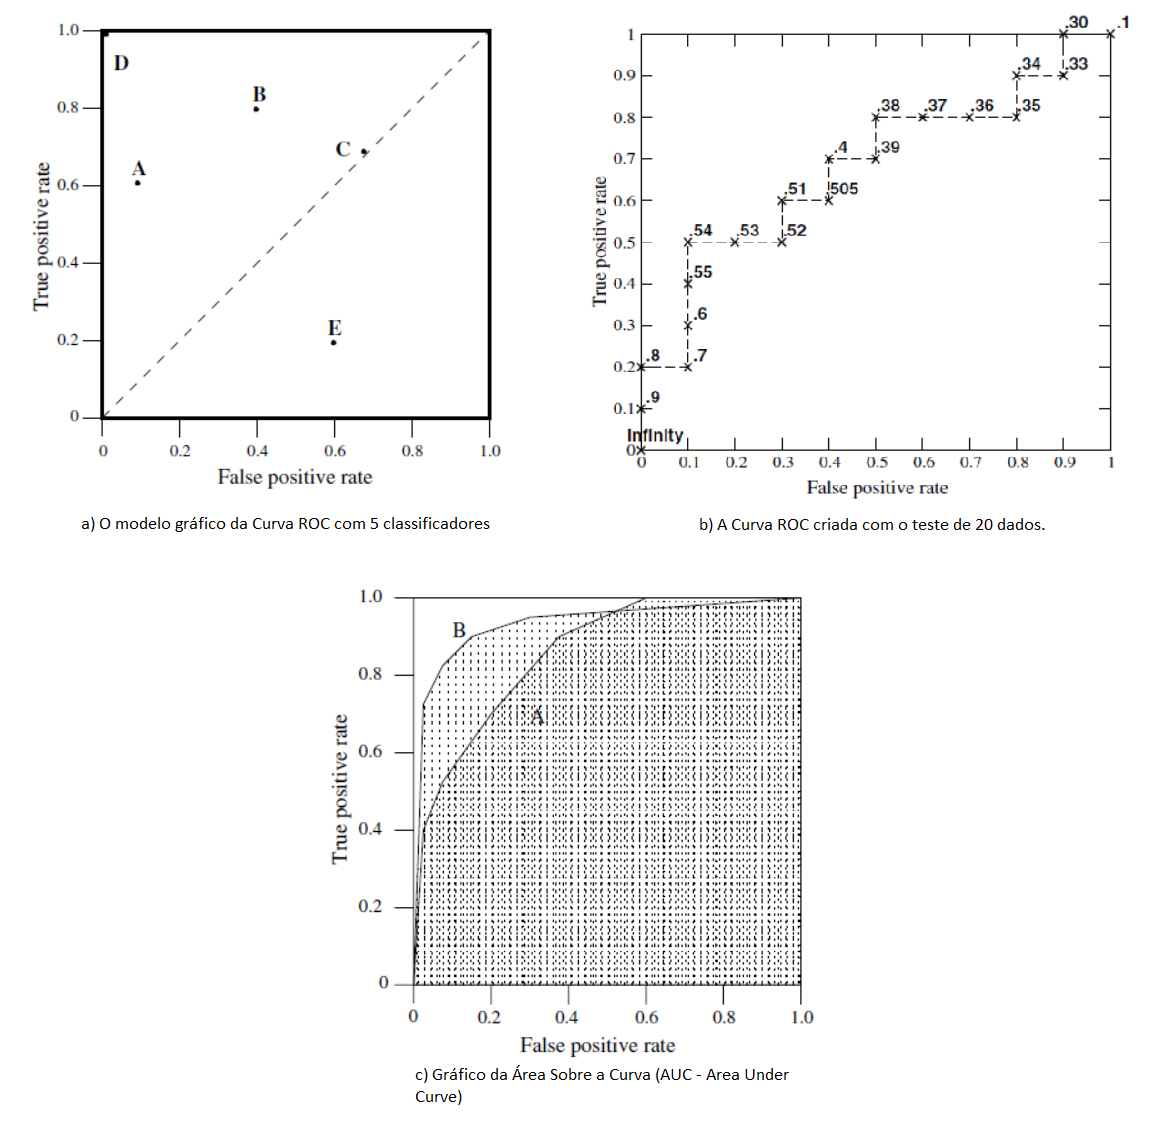
\includegraphics[width=0.8\linewidth]{curvaroc} 

}

\caption{Curva ROC}\label{fig:curvaroc}
\end{figure}

Fonte: Adaptado de FAWCETT (\protect\hyperlink{ref-Fawcett2006}{2006}).

A Figura \ref{fig:curvaroc}b mostra a formação da curva ROC para um teste com 20 instâncias, uma amostra pequena servindo portanto de exemplificação da sua criação. Para isto, o modelo de regressão logística é rodado randomicamente e a predição resultante é comparada com o valor real da variável dependente. O ponto de corte padrão, como visto anteriormente, é o valor de 0,5: acima deste valor, a predição é classificada como 1 e, abaixo dele 0. Na Figura \ref{fig:curvaroc}b, a primeira predição foi 0,9 e a segunda 0,8 sendo que como estão mais perto do eixo X do gráfico, representam predições acertadas. Já para predições que não foram acertadas (como no exemplo as predições 0,7 e 0,54 por exemplo) a curva caminha para a direita. A lógica se mantém até o final da elaboração da curva.

Já na Figura \ref{fig:curvaroc}c é demonstrada a elaboração do conceito da Área sobre a Curva ROC (AUC - Area Under the ROC Curve), que objetiva comparar os classificadores a partir da parformance da curva em um único valor escalar (FAWCETT, \protect\hyperlink{ref-Fawcett2006}{2006}). Este indicador representa a probabilidade de que o classificador efetue predições randômicas na instância positiva melhor do que na instância negativa.
O indicador AUC sempre terá seu valor entre 0 e 1, sendo que quanto maior, melhor e nunca um classificador realístico deve estar abaixo de 0,5. HOSMER; LEMESCHOW (\protect\hyperlink{ref-Hosmer2000}{2000}) sugere a utilização de AUC acima de 0,7 como aceitável. Como exemplo, a Figura \ref{fig:curvaroc}c mostra que a curva ROC B tem uma melhor capacidade preditiva que a curva A.

Seguem os passos para elaboração da curva ROC.

\begin{itemize}
\tightlist
\item
  Passo 1:
\end{itemize}

\texttt{require(pROC)}

\texttt{roc1=plot.roc(chd\$CHD,fitted(m1))}

\begin{itemize}
\tightlist
\item
  Passo 2:
\end{itemize}

\begin{Shaded}
\begin{Highlighting}[]
\KeywordTok{plot}\NormalTok{(roc1,}
     \DataTypeTok{print.auc=}\OtherTok{TRUE}\NormalTok{, }
     \DataTypeTok{auc.polygon=}\OtherTok{TRUE}\NormalTok{, }
     \DataTypeTok{grud=}\KeywordTok{c}\NormalTok{(}\FloatTok{0.1}\NormalTok{,}\FloatTok{0.2}\NormalTok{),}
     \DataTypeTok{grid.col=}\KeywordTok{c}\NormalTok{(}\StringTok{"green"}\NormalTok{,}\StringTok{"red"}\NormalTok{), }
     \DataTypeTok{max.auc.polygon=}\OtherTok{TRUE}\NormalTok{, }
     \DataTypeTok{auc.polygon.col=}\StringTok{"lightgreen"}\NormalTok{, }
     \DataTypeTok{print.thres=}\OtherTok{TRUE}\NormalTok{)}
\end{Highlighting}
\end{Shaded}

\begin{figure}[H]

{\centering 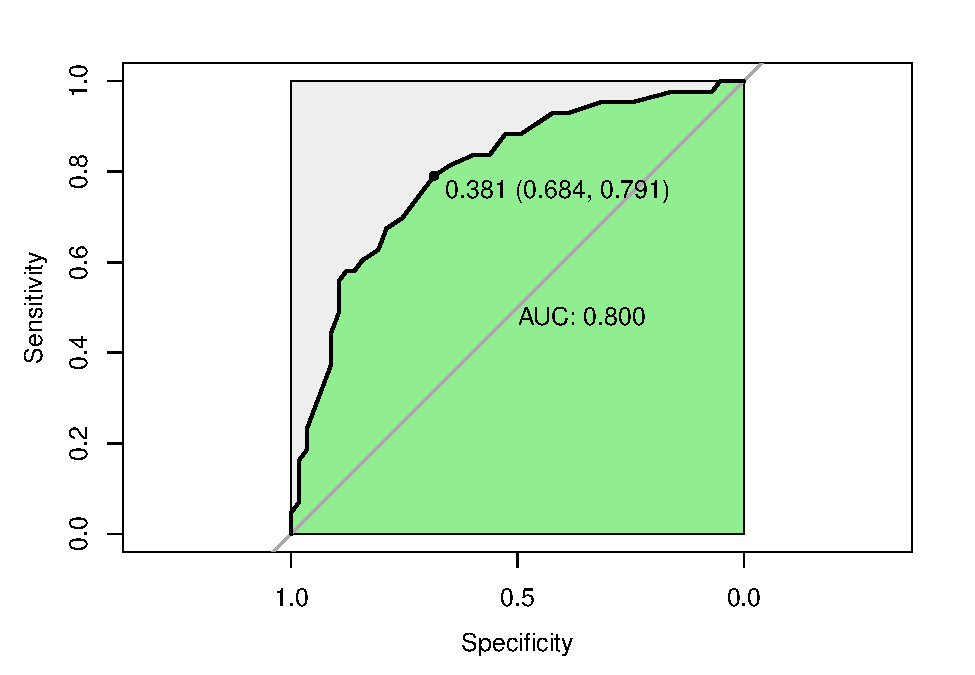
\includegraphics[width=0.8\linewidth]{index_files/figure-latex/roc-1} 

}

\caption{Curva Roc}\label{fig:roc}
\end{figure}

\hypertarget{o-teste-hosmer-e-lemeshow}{%
\subsection{O teste Hosmer e Lemeshow}\label{o-teste-hosmer-e-lemeshow}}

O teste de Hosmer e Lemeshow é utilizado para demonstrar a qualidade do ajuste do modelo, ou seja, se o modelo pode explicar os dados observados. Para este teste, os dados são divididos de acordo com as probabilidades previstas em 10 grupos iguais, sendo que os números previstos e os reais são comparados com a estatística do qui-quadrado. HAIR et al. (\protect\hyperlink{ref-Hair2009}{2009}) sugerem um tamanho de amostra de pelo menos 50 casos para a realização deste teste.

A hipótese nula H\({_0}\) do qui-quadrado (\texttt{p=0,05}) deste teste é a de que as proporções observadas e esperadas são as mesmas ao longo da amostra. Abaixo segue a estrutura do teste, sendo que o modelo apresenta dificuldade de ajuste em função de que rejeita a hipótese nula a \emph{p=0,05}.

\begin{Shaded}
\begin{Highlighting}[]
\KeywordTok{require}\NormalTok{(ResourceSelection)}
\NormalTok{hl=}\KeywordTok{hoslem.test}\NormalTok{(chd}\OperatorTok{$}\NormalTok{CHD,}\KeywordTok{fitted}\NormalTok{(m1),}\DataTypeTok{g=}\DecValTok{10}\NormalTok{)}
\NormalTok{hl}
\end{Highlighting}
\end{Shaded}

\begin{verbatim}

    Hosmer and Lemeshow goodness of fit (GOF) test

data:  chd$CHD, fitted(m1)
X-squared = 100, df = 8, p-value <2e-16
\end{verbatim}

\hypertarget{pseudo-r2}{%
\subsection{\texorpdfstring{Pseudo R\(^2\)}{Pseudo R\^{}2}}\label{pseudo-r2}}

Semelhante ao coeficiente de determinação R\({^2}\) da regressão múltipla, a medida de pseudo R\({^2}\) representam o ajuste geral do modelo proposto. Sua interpretação, portanto, é semelhante à regressão múltipla. Abaixo segue o cálculo do pseudo R\({^2}\):

\[
R{^2}_{LOGIT} = \frac{-2LL_{nulo}-(-2LL_{modelo})}{-2LL_{nulo}}
\]
Lembrando que o valor -2LL representa -2 vezes o logaritmo do valor de verossimilhança, onde a verossimilhança do modelo nulo é comparado com o modelo completo. Abaixo mostra-se o código para calcular os indicadores, sendo que constam as medidas de pseudo R\({^2}\) estipuladas por Cox e Snell, Nagelkerke e McFadden.

\begin{Shaded}
\begin{Highlighting}[]
\KeywordTok{require}\NormalTok{(modEvA)}
\KeywordTok{RsqGLM}\NormalTok{(m1)}
\end{Highlighting}
\end{Shaded}

\begin{verbatim}
$CoxSnell
[1] 0.2541

$Nagelkerke
[1] 0.341

$McFadden
[1] 0.2145

$Tjur
[1] 0.2706

$sqPearson
[1] 0.2726
\end{verbatim}

\hypertarget{regressao-logistica-multipla}{%
\section{Regressão Logística Múltipla}\label{regressao-logistica-multipla}}

O exemplo abaixo abordado foi extraído de TORRES-REYNA (\protect\hyperlink{ref-Torres-Reyna2014}{2014}), onde observa-se o banco de dados criado chamado \texttt{mydata}, possuindo as variáveis\texttt{country},\texttt{year},\texttt{y},\texttt{y\_bin},\texttt{x1},\texttt{x2},\texttt{x3} e\texttt{opinion}. A variável dependente é \texttt{y\_bin}, da qual foi categorizada entre 0 e 1 conforme a ocorrência de valores negativos em\texttt{y}. As variáveis independentes do modelo serão\texttt{x1},\texttt{x2}e\texttt{x3}.

\begin{Shaded}
\begin{Highlighting}[]
\KeywordTok{require}\NormalTok{(haven)}
\end{Highlighting}
\end{Shaded}

\begin{verbatim}
Carregando pacotes exigidos: haven
\end{verbatim}

\begin{Shaded}
\begin{Highlighting}[]
\NormalTok{mydata <-}\StringTok{ }\KeywordTok{read_dta}\NormalTok{(}\StringTok{"http://dss.princeton.edu/training/Panel101.dta"}\NormalTok{) }
\KeywordTok{summary}\NormalTok{(mydata)}
\end{Highlighting}
\end{Shaded}

\begin{verbatim}
    country       year            y                 y_bin           x1        
 Min.   :1   Min.   :1990   Min.   :-7.86e+09   Min.   :0.0   Min.   :-0.568  
 1st Qu.:2   1st Qu.:1992   1st Qu.: 2.47e+08   1st Qu.:1.0   1st Qu.: 0.329  
 Median :4   Median :1994   Median : 1.90e+09   Median :1.0   Median : 0.641  
 Mean   :4   Mean   :1994   Mean   : 1.85e+09   Mean   :0.8   Mean   : 0.648  
 3rd Qu.:6   3rd Qu.:1997   3rd Qu.: 3.37e+09   3rd Qu.:1.0   3rd Qu.: 1.096  
 Max.   :7   Max.   :1999   Max.   : 8.94e+09   Max.   :1.0   Max.   : 1.446  
       x2               x3            opinion    
 Min.   :-1.622   Min.   :-1.165   Min.   :1.00  
 1st Qu.:-1.216   1st Qu.:-0.079   1st Qu.:1.00  
 Median :-0.462   Median : 0.514   Median :2.50  
 Mean   : 0.134   Mean   : 0.762   Mean   :2.44  
 3rd Qu.: 1.608   3rd Qu.: 1.155   3rd Qu.:3.00  
 Max.   : 2.530   Max.   : 7.169   Max.   :4.00  
\end{verbatim}

Utiliza-se uma função para Modelos Lineares Generalizados (glm - em inglês Generalized Linear Models), determinando a variável dependente (y\_bin), as variáveis independentes \texttt{(x1+x2+x3)}, a base de dados a ser utilizada \texttt{(data=mydata)} e a família dos modelos \texttt{(family\ =\ binomial(link="logit"))}.

Abaixo os resultados da estimação do modelo utilizando o comando \texttt{summary}. Observa-se que os valores \texttt{estimados} mostram os coeficientes em formato logarítmo de chances. Assim, quando x3 eleva-se em 1 (uma) unidade, o log das chances esperado para x3 altera-se em 0,7512. Neste ponto, observa-se que as três variáveis independentes possuem efeitos positivos para determinação das chances do preditor ser igual a 1, caso contrário constariam com sinal negativo. A coluna \(Pr(>|z|)\) traz os p-valores das variáveis indicando o teste da hipótese nula. Como resultado a variável x3 revelou significância estatística a 10\% (\$\textless{}\$0,10), no entanto o valor usual para considerá-la estatísticamente significante é 5\% (0,05). Para fins de explanação do modelo, neste trabalho, serão efetuadas as demais análises do modelo de forma explicativa.

\begin{Shaded}
\begin{Highlighting}[]
\NormalTok{logit=}\KeywordTok{glm}\NormalTok{(y_bin}\OperatorTok{~}\NormalTok{x1}\OperatorTok{+}\NormalTok{x2}\OperatorTok{+}\NormalTok{x3, }\DataTypeTok{data=}\NormalTok{mydata, }\DataTypeTok{family =} \KeywordTok{binomial}\NormalTok{(}\DataTypeTok{link=}\StringTok{"logit"}\NormalTok{))}
\KeywordTok{summary}\NormalTok{(logit)}
\end{Highlighting}
\end{Shaded}

\begin{verbatim}

Call:
glm(formula = y_bin ~ x1 + x2 + x3, family = binomial(link = "logit"), 
    data = mydata)

Deviance Residuals: 
   Min      1Q  Median      3Q     Max  
-2.028   0.235   0.554   0.702   1.084  

Coefficients:
            Estimate Std. Error z value Pr(>|z|)  
(Intercept)    0.426      0.639    0.67    0.505  
x1             0.862      0.784    1.10    0.272  
x2             0.367      0.308    1.19    0.234  
x3             0.751      0.455    1.65    0.099 .
---
Signif. codes:  0 '***' 0.001 '**' 0.01 '*' 0.05 '.' 0.1 ' ' 1

(Dispersion parameter for binomial family taken to be 1)

    Null deviance: 70.056  on 69  degrees of freedom
Residual deviance: 65.512  on 66  degrees of freedom
AIC: 73.51

Number of Fisher Scoring iterations: 5
\end{verbatim}

\begin{Shaded}
\begin{Highlighting}[]
\KeywordTok{require}\NormalTok{(stargazer)}
\KeywordTok{stargazer}\NormalTok{(logit, }\DataTypeTok{title=}\StringTok{"Resultados"}\NormalTok{,}\DataTypeTok{type =} \StringTok{"text"}\NormalTok{)}
\end{Highlighting}
\end{Shaded}

\begin{verbatim}

Resultados
=============================================
                      Dependent variable:    
                  ---------------------------
                             y_bin           
---------------------------------------------
x1                           0.862           
                            (0.784)          
                                             
x2                           0.367           
                            (0.308)          
                                             
x3                          0.751*           
                            (0.455)          
                                             
Constant                     0.426           
                            (0.639)          
                                             
---------------------------------------------
Observations                  70             
Log Likelihood              -32.760          
Akaike Inf. Crit.           73.510           
=============================================
Note:             *p<0.1; **p<0.05; ***p<0.01
\end{verbatim}

A razão de chances (OR - odds ratio em inglês) estimada no modelo terá de ser transformada por estar apresentada na forma logarítma conforme o modelo de regressão logística o estima. Assim, utiliza-se o pacote \texttt{mfx} para efetuar esta transformação para todo o modelo de forma automatizada \texttt{(logitor(y\_bin\textasciitilde{}x1+x2+x3,data=mydata))}:

\begin{Shaded}
\begin{Highlighting}[]
\KeywordTok{require}\NormalTok{(mfx)}
\KeywordTok{logitor}\NormalTok{(y_bin}\OperatorTok{~}\NormalTok{x1}\OperatorTok{+}\NormalTok{x2}\OperatorTok{+}\NormalTok{x3,}\DataTypeTok{data=}\NormalTok{mydata)}
\end{Highlighting}
\end{Shaded}

\begin{verbatim}
Call:
logitor(formula = y_bin ~ x1 + x2 + x3, data = mydata)

Odds Ratio:
   OddsRatio Std. Err.    z P>|z|  
x1     2.367     1.856 1.10 0.272  
x2     1.443     0.445 1.19 0.234  
x3     2.120     0.964 1.65 0.099 .
---
Signif. codes:  0 '***' 0.001 '**' 0.01 '*' 0.05 '.' 0.1 ' ' 1
\end{verbatim}

O resultado acima evidencia que para uma alteração em 1 (uma) unidade em x3, a chance de que y seja igual a 1 aumenta em 112\% ((2,12-1)*100). Dito de outra forma, a chance de y=1 é 2,12 vezes maior quando x3 aumenta em uma unidade (sendo que aqui mantêm-se as demais variáveis independentes constantes).

Como visto, para cada variação unitária em x3 o log das chances varia 0,7512. É possível estimar, portanto, a alteração das chances em função das médias dos valores de cada variável x1 e x2, e utilizar como exemplo os valores de 1, 2 e 3 para x3, para assim alcançar os preditores do log das chances nesta simulação, como segue abaixo:

Para facilitar a interpretação do modelo, se torna mais fácil depois de transformado a sua exponenciação dos coeficientes logísticos utilizando o comando \texttt{exp(coef(logit))}. Desta forma, para cada incremento unitário em x2 e mantendo as demais variáveis constantes, conclui-se que é 1,443 vezes provável que y seja igual a 1 em oposição a não ser (igual a zero), ou seja, as chances aumentam em 44,30\%.

\begin{Shaded}
\begin{Highlighting}[]
\KeywordTok{exp}\NormalTok{(}\KeywordTok{coef}\NormalTok{(logit))}
\end{Highlighting}
\end{Shaded}

\begin{verbatim}
(Intercept)          x1          x2          x3 
      1.531       2.367       1.443       2.120 
\end{verbatim}

O \textbf{intervalo de confiança} do modelo pode ser exposto utilizando o comando \texttt{confint} para os coeficientes estimados, como segue abaixo:

\begin{Shaded}
\begin{Highlighting}[]
\KeywordTok{exp}\NormalTok{(}\KeywordTok{cbind}\NormalTok{(}\DataTypeTok{OR=}\KeywordTok{coef}\NormalTok{(logit), }\KeywordTok{confint}\NormalTok{(logit)))}
\end{Highlighting}
\end{Shaded}

\begin{verbatim}
               OR  2.5 % 97.5 %
(Intercept) 1.531 0.4387  5.625
x1          2.367 0.5129 11.675
x2          1.443 0.8041  2.738
x3          2.120 1.0039  5.719
\end{verbatim}

A partir do modelo logístico, podemos realizar \textbf{predições das probabilidades} de se encontrar o resultado y=1 conforme visto acima. Para isto, como exercício utilizaremos as médias das observações de cada variável independente do modelo. Em primeiro lugar deve ser criado um data.frame com os valores médios, como segue:

\begin{Shaded}
\begin{Highlighting}[]
\NormalTok{allmean =}\StringTok{ }\KeywordTok{data.frame}\NormalTok{(}\DataTypeTok{x1=}\KeywordTok{mean}\NormalTok{(mydata}\OperatorTok{$}\NormalTok{x1),}
                     \DataTypeTok{x2=}\KeywordTok{mean}\NormalTok{(mydata}\OperatorTok{$}\NormalTok{x2),}
                     \DataTypeTok{x3=}\KeywordTok{mean}\NormalTok{(mydata}\OperatorTok{$}\NormalTok{x3))}
\NormalTok{allmean}
\end{Highlighting}
\end{Shaded}

\begin{verbatim}
     x1     x2     x3
1 0.648 0.1339 0.7619
\end{verbatim}

Utiliza-se o comando \texttt{predict()} para predição do modelo, como segue abaixo, informando o objeto criado com a equação do modelo (logit), a base de dados com as condições dos valores médios (allmean) e o tipo de teste requerido (``response'') para predizer as probabilidades. Como resultado, o modelo informa que constando os valores médios das variáveis independentes, obtêm-se a probabilidade de 83\% em y se constituir igual a 1.

\begin{Shaded}
\begin{Highlighting}[]
\NormalTok{allmean}\OperatorTok{$}\NormalTok{pred.prob =}\StringTok{ }\KeywordTok{predict}\NormalTok{(logit, }\DataTypeTok{newdata=}\NormalTok{allmean, }\DataTypeTok{type=}\StringTok{"response"}\NormalTok{)}
\NormalTok{allmean}
\end{Highlighting}
\end{Shaded}

\begin{verbatim}
     x1     x2     x3 pred.prob
1 0.648 0.1339 0.7619    0.8329
\end{verbatim}

\hypertarget{metodo-stepwise}{%
\subsection{Método Stepwise}\label{metodo-stepwise}}

O método Stepwise auxilia o pesquisador em selecionar as variáveis importantes ao modelo, sendo que podem ser utilizadas nas direções ``both'', ``backward'', ``forward''. Este método, por sua vez, utiliza o Critério de Informação de Akaike (AIC - Akaike Information Criterion) na combinação das variáveis dos diversos modelos simulados para selecionar o modelo mais ajustado. Quanto menor o AIC, melhor o ajuste do modelo. O AIC é calculado da seguitne forma:

\[
AIC = -2log(L_{p})+2[(p+1)+1]
\]
onde \(L_{p}\) é a função de máxima verossimilhança e \(p\) é o número de variáveis explicativas do modelo. Segue o código para execução no console:

\begin{Shaded}
\begin{Highlighting}[]
\KeywordTok{step}\NormalTok{(logit, }\DataTypeTok{direction =} \StringTok{'both'}\NormalTok{)}
\end{Highlighting}
\end{Shaded}

\begin{verbatim}
Start:  AIC=73.51
y_bin ~ x1 + x2 + x3

       Df Deviance  AIC
- x1    1     66.7 72.7
- x2    1     67.0 73.0
<none>        65.5 73.5
- x3    1     69.4 75.4

Step:  AIC=72.74
y_bin ~ x2 + x3

       Df Deviance  AIC
- x2    1     67.3 71.3
<none>        66.7 72.7
+ x1    1     65.5 73.5
- x3    1     70.0 74.0

Step:  AIC=71.33
y_bin ~ x3

       Df Deviance  AIC
<none>        67.3 71.3
- x3    1     70.1 72.1
+ x2    1     66.7 72.7
+ x1    1     67.0 73.0
\end{verbatim}

\begin{verbatim}

Call:  glm(formula = y_bin ~ x3, family = binomial(link = "logit"), 
    data = mydata)

Coefficients:
(Intercept)           x3  
      1.134        0.487  

Degrees of Freedom: 69 Total (i.e. Null);  68 Residual
Null Deviance:      70.1 
Residual Deviance: 67.3     AIC: 71.3
\end{verbatim}

\hypertarget{vif---variance-inflation-factor}{%
\subsection{VIF - Variance Inflation Factor}\label{vif---variance-inflation-factor}}

Os problemas de multicolinearedade nos modelos de regressão, ou seja, as relações entre as variáveis do modelo, podem prejudicar a capacidade preditiva do mesmo. Nas palavras de HAIR et al. (\protect\hyperlink{ref-Hair2009}{2009}, p. 191), ``multicolinearidade cria variância ``compartilhada'' entre variáveis, diminuindo assim a capacidade de prever a medida dependente, bem como averiguar os papéis relativos de cada variável independente".
Para resolver esta questão, utiliza-se o teste do fator de inflação da variância (VIF - Variance Inflation Factor), índice o qual não deve ficar abaixo de 10 para representar baixo problema de multicolinearidade segundo RAWLINGS; PANTULA; DICKEY (\protect\hyperlink{ref-Rawlings1998}{1998}).

\begin{Shaded}
\begin{Highlighting}[]
\KeywordTok{require}\NormalTok{(faraway)}
\KeywordTok{vif}\NormalTok{(logit)}
\end{Highlighting}
\end{Shaded}

\begin{verbatim}
    x1     x2     x3 
 9.292 12.318 29.860 
\end{verbatim}

\hypertarget{regressao-logistica-multipla-com-variavel-categorica}{%
\section{Regressão Logística Múltipla com variável categórica}\label{regressao-logistica-multipla-com-variavel-categorica}}

Agora segue um exemplo de regressão logística utilizando uma variável dependente categórica juntamente com variáveis numéricas. Trata-se de uma base de dados em que o interesse é descobrir a probabilidade de um aluno ser admitido no vestibular com base no ranqueamento de escola em que estudou no ensino médio, bem como nas notas do aluno nas provas do Gpa (Grade Point Average - uma nota de performance dos alunos nos Estados Unidos) e do Gre (Graduate Record Examinations - exame padrão que qualifica o estudante para o ensino superior nos Estados Unidos). Seguem as variáveis.

\begin{itemize}
\tightlist
\item
  \textbf{admin}: Variável dependente = 0 (não admitido) e 1 (admitido)
\item
  \textbf{Rank}: Variável independente = ranking da escola de proveniência do candidato
\item
  \textbf{Gre}: Variável independente = exames prévios do candidato.
\item
  \textbf{Gpa}: Variável independente = exames prévios do candidato.
\end{itemize}

Abaixo seguem os resultados do modelo, partindo-se do carregamento dos dados. É observado que as variáveis \textbf{gre} e \textbf{gpa} obtiveram significância estatística em 10\%, bem como rank2, já rank3 e rank4 obtiveram \texttt{p=0,001}. A variância do modelo nulo
ficou em 499,98 e com a inclusão das variáveis ao modelo baixou para 458,52, o que mostra que contribuíram para explicação da variável dependente.

\begin{Shaded}
\begin{Highlighting}[]
\CommentTok{# Carregando o arquivo}
\KeywordTok{require}\NormalTok{(readr)}
\NormalTok{binary <-}\StringTok{ }\KeywordTok{read_csv}\NormalTok{(}\StringTok{"http://www.karlin.mff.cuni.cz/~pesta/prednasky/NMFM404/Data/binary.csv"}\NormalTok{)}

\CommentTok{# Transformando a variável rank em categórica}
\NormalTok{binary}\OperatorTok{$}\NormalTok{rank <-}\StringTok{ }\KeywordTok{factor}\NormalTok{(binary}\OperatorTok{$}\NormalTok{rank)}

\CommentTok{# Determinando a regressão}
\NormalTok{mylogit <-}\StringTok{ }\KeywordTok{glm}\NormalTok{(admit }\OperatorTok{~}\StringTok{ }\NormalTok{gre }\OperatorTok{+}\StringTok{ }\NormalTok{gpa }\OperatorTok{+}\StringTok{ }\NormalTok{rank, }\DataTypeTok{data =}\NormalTok{ binary, }
               \DataTypeTok{family =} \KeywordTok{binomial}\NormalTok{(}\DataTypeTok{link=}\StringTok{"logit"}\NormalTok{))}

\CommentTok{# Resultado}
\KeywordTok{summary}\NormalTok{(mylogit)}
\end{Highlighting}
\end{Shaded}

\begin{verbatim}

Call:
glm(formula = admit ~ gre + gpa + rank, family = binomial(link = "logit"), 
    data = binary)

Deviance Residuals: 
   Min      1Q  Median      3Q     Max  
-1.627  -0.866  -0.639   1.149   2.079  

Coefficients:
            Estimate Std. Error z value Pr(>|z|)    
(Intercept) -3.98998    1.13995   -3.50  0.00047 ***
gre          0.00226    0.00109    2.07  0.03847 *  
gpa          0.80404    0.33182    2.42  0.01539 *  
rank2       -0.67544    0.31649   -2.13  0.03283 *  
rank3       -1.34020    0.34531   -3.88  0.00010 ***
rank4       -1.55146    0.41783   -3.71  0.00020 ***
---
Signif. codes:  0 '***' 0.001 '**' 0.01 '*' 0.05 '.' 0.1 ' ' 1

(Dispersion parameter for binomial family taken to be 1)

    Null deviance: 499.98  on 399  degrees of freedom
Residual deviance: 458.52  on 394  degrees of freedom
AIC: 470.5

Number of Fisher Scoring iterations: 4
\end{verbatim}

Utilizando o teste de análise de variância \texttt{anova} pode-se observar a variância com o modelo nulo (500) e à medida que as variáveis explicativas foram sendo incluídas, estas reduziram a variância do modelo para 459, contribuindo para o modelo.

\begin{Shaded}
\begin{Highlighting}[]
\KeywordTok{anova}\NormalTok{(mylogit, }\DataTypeTok{test =} \StringTok{"Chisq"}\NormalTok{)}
\end{Highlighting}
\end{Shaded}

\begin{verbatim}
Analysis of Deviance Table

Model: binomial, link: logit

Response: admit

Terms added sequentially (first to last)

     Df Deviance Resid. Df Resid. Dev Pr(>Chi)    
NULL                   399        500             
gre   1    13.92       398        486  0.00019 ***
gpa   1     5.71       397        480  0.01685 *  
rank  3    21.83       394        459  7.1e-05 ***
---
Signif. codes:  0 '***' 0.001 '**' 0.01 '*' 0.05 '.' 0.1 ' ' 1
\end{verbatim}

Caso seja interessante comparar diversos modelos de regressão com variáveis explicativas distintas, estes podem ser comparados no teste de variância \texttt{anova}. Utilizando a função \texttt{update} pode ser criada uma nova regressão com base na regressão anterior (\texttt{mylogit}) e é excluído do modelo a variável \texttt{gre} para exemplificar. Após, é efetuado novamente o teste \texttt{anova}, agora comparando os dois modelos, como segue abaixo. Evidencia-se que a exclusão da variável \texttt{gre} causou elevaçãod a variância do modelo para 463, piorando portanto a capacidade do modelo pois espera-se sempre reduções na sua variância.

\begin{Shaded}
\begin{Highlighting}[]
\CommentTok{# Criação de novo modelo com base no anterior}
\NormalTok{mylogit2=}\KeywordTok{update}\NormalTok{(mylogit,}\OperatorTok{~}\NormalTok{. }\OperatorTok{-}\StringTok{ }\NormalTok{gre)}
\CommentTok{# }
\KeywordTok{anova}\NormalTok{(mylogit,mylogit2, }\DataTypeTok{test =} \StringTok{"Chisq"}\NormalTok{)}
\end{Highlighting}
\end{Shaded}

\begin{verbatim}
Analysis of Deviance Table

Model 1: admit ~ gre + gpa + rank
Model 2: admit ~ gpa + rank
  Resid. Df Resid. Dev Df Deviance Pr(>Chi)  
1       394        459                       
2       395        463 -1    -4.36    0.037 *
---
Signif. codes:  0 '***' 0.001 '**' 0.01 '*' 0.05 '.' 0.1 ' ' 1
\end{verbatim}

Voltando ao modelo determinado anteriormente (\texttt{mylogit}), observa-se que os parâmetros da regressão logística proposta utilizando todas as variáveis foram assim determinados:

\[
ln(P=Y) = 
-3,98998 + 0.00226gre + 0,80404gpa -0,67544rank2 -1,34020rank3 -1,55146rank4
\]

Determinam-se os coeficientes exponenciados (as razões de chance) para cada variável do modelo, bem como seus intervalos de confiança:

\begin{Shaded}
\begin{Highlighting}[]
\KeywordTok{exp}\NormalTok{(}\KeywordTok{cbind}\NormalTok{(}\DataTypeTok{OR =} \KeywordTok{coef}\NormalTok{(mylogit), }\KeywordTok{confint}\NormalTok{(mylogit)))}
\end{Highlighting}
\end{Shaded}

\begin{verbatim}
                OR    2.5 % 97.5 %
(Intercept) 0.0185 0.001889 0.1665
gre         1.0023 1.000138 1.0044
gpa         2.2345 1.173858 4.3238
rank2       0.5089 0.272290 0.9448
rank3       0.2618 0.131642 0.5115
rank4       0.2119 0.090716 0.4707
\end{verbatim}

A leitura dos resultados, para as variáveis numéricas continua sendo a mesma. Com relação ao resultado para a variável \textbf{gre}, para cada aumento unitário nesta variável, mantendo-se as demais constantes, elevam-se em 0,23\% ((1,0023-1)*100) as chances de que o aluno seja aprovado no vestibular. Já para a cada variação unitária na variável \textbf{gpa}, aumentam em 123,45\% ((2,2345-1)*100).
Dito de outra forma, para cada elevação em \textbf{gpa} aumentam 2,2345 vezes as chances em ser aprovado no vestibular. Tais resultados vão de encontro ao conceito teórico de que quanto melhor a nota do aluno em exame prévios maiores as chances de este aluno passar no vestibular.

Outra questão é sobre o \emph{ranking} das escolas que os alunos estudaram. Será que aqueles que estudaram em escolas melhores ranqueadas possuem mais chances de passar no vestibular? A variável \textbf{rank} traz esta análise, sendo que como é uma variável categórica (pois retoma as categorias de 1 a 4), as comparações das chances de que o aluno passe no vestibular são comparadas com a escola de \emph{ranking} 1.

Desta forma, em sendo o aluno proveniente de uma escola de \emph{ranking} 2, diminuem-se as chances em 49,11\% ((0,5089-1)\$\emph{\$100) de que o aluno passe no vestibular. Já para os alunos que estudaramem uma escola de }ranking* 3 tem 73,82\% ((0,2618-1)*100) menos chances de passar no vestibular.
Pioram ainda mais as chances de passar no vestibular daqueles alunos que estudaram em uma escola de \emph{ranking} 4: diminuem-se em 78,81\% as chances de que estes aluno passe no vestibular, mantidas as demais veriáveis.

\textbf{Predição das probabilidades}: a partir da equação de regressão logística auferida neste exemplo, qual é a probabilidade de que um aluno que tirou nota no \textbf{gre} de 700, no \textbf{gpa} de 3,67 e estudou em uma escola de \emph{ranking} 1 passe no vestibular?
Nota-se que a probabilidade de que este aluno passe no vestibular é de 63,32\%. Segue a predição para estas variáveis:

\begin{Shaded}
\begin{Highlighting}[]
\NormalTok{pred=}\KeywordTok{data.frame}\NormalTok{(}\DataTypeTok{gre=}\DecValTok{700}\NormalTok{,}
                \DataTypeTok{gpa=}\FloatTok{3.67}\NormalTok{,}
                \DataTypeTok{rank=}\KeywordTok{factor}\NormalTok{(}\DecValTok{1}\NormalTok{)}
\NormalTok{                )}
\NormalTok{pred}\OperatorTok{$}\NormalTok{prob=}\KeywordTok{predict}\NormalTok{(mylogit, }\DataTypeTok{newdata=}\NormalTok{pred, }\DataTypeTok{type=}\StringTok{"response"}\NormalTok{)}
\NormalTok{pred}
\end{Highlighting}
\end{Shaded}

\begin{verbatim}
  gre  gpa rank   prob
1 700 3.67    1 0.6332
\end{verbatim}

Comparando com um aluno que tirou as mesmas notas no \textbf{gre} e \textbf{gpa}, mas que estudou em uma escola \emph{ranking} 4:

\begin{Shaded}
\begin{Highlighting}[]
\NormalTok{pred=}\KeywordTok{data.frame}\NormalTok{(}\DataTypeTok{gre=}\DecValTok{700}\NormalTok{,}
                \DataTypeTok{gpa=}\FloatTok{3.67}\NormalTok{,}
                \DataTypeTok{rank=}\KeywordTok{factor}\NormalTok{(}\DecValTok{4}\NormalTok{)}
\NormalTok{                )}
\NormalTok{pred}\OperatorTok{$}\NormalTok{prob=}\KeywordTok{predict}\NormalTok{(mylogit, }\DataTypeTok{newdata=}\NormalTok{pred, }\DataTypeTok{type=}\StringTok{"response"}\NormalTok{)}
\NormalTok{pred}
\end{Highlighting}
\end{Shaded}

\begin{verbatim}
  gre  gpa rank   prob
1 700 3.67    4 0.2679
\end{verbatim}

Agora será efetuada a predição comparando-se os \emph{rankings} das escolas. No exemplo abaixo, é criada uma base de dados com as notas médias dos alunos nas variáveis \textbf{gre} e \textbf{gpa}, intercalando com todos os \emph{rankings} das escolas onde estudaram. Após criar a tabela, esta é unida com as colunas de predição dos valores da equação. São renomeadas as variáveis de \emph{fit} para \emph{prob} e \emph{se.fit} para \emph{se.prob}, no primeiro caso pois obteiveram-se as probabilidades de cada caso e no segundo caso incluiu-se o erro padrão (\emph{se: standart error}) desta probabilidade. Com este erro padrão calculou-se os limites inferior (\emph{LL: low level}) e superior (\emph{UL: upper level }) no intervalo de confiança de 95\%.

\begin{Shaded}
\begin{Highlighting}[]
\CommentTok{# Criação da tabela}
\NormalTok{novosdados=}\KeywordTok{with}\NormalTok{(binary,}
                \KeywordTok{data.frame}\NormalTok{(}\DataTypeTok{gre=}\KeywordTok{mean}\NormalTok{(gre),}
                           \DataTypeTok{gpa=}\KeywordTok{mean}\NormalTok{(gpa),}
                           \DataTypeTok{rank=}\KeywordTok{factor}\NormalTok{(}\DecValTok{1}\OperatorTok{:}\DecValTok{4}\NormalTok{)))}

\CommentTok{# Incluindo a predição dos valores}
\NormalTok{novosdados=}\KeywordTok{cbind}\NormalTok{(novosdados,}\KeywordTok{predict}\NormalTok{(mylogit, }
                                    \DataTypeTok{newdata=}\NormalTok{novosdados,}
                                    \DataTypeTok{type=}\StringTok{"response"}\NormalTok{,}
                                    \DataTypeTok{se.fit=}\OtherTok{TRUE}\NormalTok{))}
\CommentTok{# Renomeando as variáveis}
\KeywordTok{names}\NormalTok{(novosdados)[}\KeywordTok{names}\NormalTok{(novosdados)}\OperatorTok{==}\StringTok{'fit'}\NormalTok{]=}\StringTok{"prob"}
\KeywordTok{names}\NormalTok{(novosdados)[}\KeywordTok{names}\NormalTok{(novosdados)}\OperatorTok{==}\StringTok{'se.fit'}\NormalTok{]=}\StringTok{"se.prob"}

\CommentTok{# Estimando os intervalos de confiança}

\NormalTok{novosdados}\OperatorTok{$}\NormalTok{LL=novosdados}\OperatorTok{$}\NormalTok{prob}\FloatTok{-1.96}\OperatorTok{*}\NormalTok{novosdados}\OperatorTok{$}\NormalTok{se.prob}
\NormalTok{novosdados}\OperatorTok{$}\NormalTok{UL=novosdados}\OperatorTok{$}\NormalTok{prob}\FloatTok{+1.96}\OperatorTok{*}\NormalTok{novosdados}\OperatorTok{$}\NormalTok{se.prob}

\CommentTok{# Vizualização dos dados}
\NormalTok{novosdados}
\end{Highlighting}
\end{Shaded}

\begin{verbatim}
    gre  gpa rank   prob se.prob residual.scale      LL     UL
1 587.7 3.39    1 0.5166 0.06632              1 0.38662 0.6466
2 587.7 3.39    2 0.3523 0.03978              1 0.27431 0.4303
3 587.7 3.39    3 0.2186 0.03825              1 0.14364 0.2936
4 587.7 3.39    4 0.1847 0.04864              1 0.08934 0.2800
\end{verbatim}

\begin{Shaded}
\begin{Highlighting}[]
\KeywordTok{require}\NormalTok{(ggplot2)}
\KeywordTok{ggplot}\NormalTok{(novosdados, }\KeywordTok{aes}\NormalTok{(}\DataTypeTok{x=}\NormalTok{rank,}\DataTypeTok{y=}\NormalTok{prob))}\OperatorTok{+}
\StringTok{  }\KeywordTok{geom_errorbar}\NormalTok{(}\KeywordTok{aes}\NormalTok{(}\DataTypeTok{ymin=}\NormalTok{LL, }\DataTypeTok{ymax=}\NormalTok{UL), }\DataTypeTok{width=}\FloatTok{0.2}\NormalTok{,}\DataTypeTok{lty=}\DecValTok{1}\NormalTok{,}\DataTypeTok{lwd=}\DecValTok{1}\NormalTok{,}\DataTypeTok{col=}\StringTok{"red"}\NormalTok{)}\OperatorTok{+}
\StringTok{  }\KeywordTok{geom_point}\NormalTok{(}\DataTypeTok{shape=}\DecValTok{18}\NormalTok{, }\DataTypeTok{size=}\DecValTok{5}\NormalTok{, }\DataTypeTok{fill=}\StringTok{"black"}\NormalTok{)}\OperatorTok{+}
\StringTok{  }\KeywordTok{scale_x_discrete}\NormalTok{(}\DataTypeTok{limits=}\KeywordTok{c}\NormalTok{(}\StringTok{"1"}\NormalTok{,}\StringTok{"2"}\NormalTok{,}\StringTok{"3"}\NormalTok{,}\StringTok{"4"}\NormalTok{))}\OperatorTok{+}
\StringTok{  }\KeywordTok{labs}\NormalTok{(}\DataTypeTok{title=}\StringTok{"Probabilidades preditas"}\NormalTok{, }\DataTypeTok{x=}\StringTok{"Ranking"}\NormalTok{,}\DataTypeTok{y=}\StringTok{"Pr(y=1)"}\NormalTok{)}
\end{Highlighting}
\end{Shaded}

\begin{center}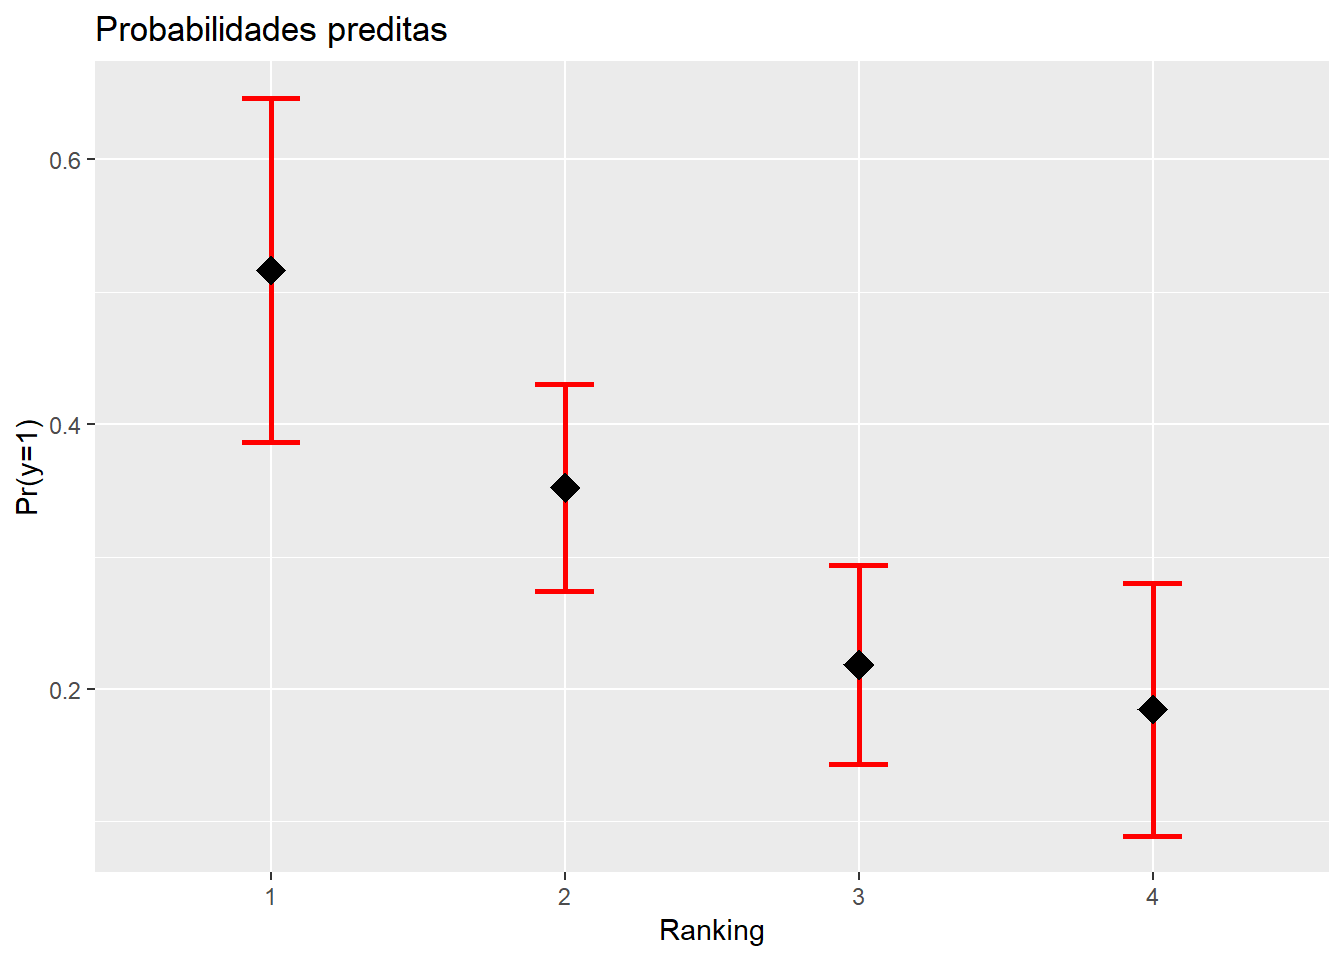
\includegraphics[width=0.8\linewidth]{index_files/figure-latex/unnamed-chunk-92-1} \end{center}

\hypertarget{exercicios}{%
\section{Exercícios}\label{exercicios}}

\textbf{1.} O Titanic foi um famoso navio britânico construído a partir de março de 1909 e lançado ao mar em maio de 1911. Em sua viagem inaugural em 10 de abril de 1912, cujo objetivo era partir de Southampton para Nova Iorque passando pela França e Irlanda, colidiu com um iceberg às 23h40min do dia 14 de abril. Baixe os dados do acidente em
\url{https://vincentarelbundock.github.io/Rdatasets/csv/COUNT/titanic.csv}. Esta base de dados possui as seguintes informações:

\begin{itemize}
\tightlist
\item
  \textbf{survived}: informa se o tripulante sobreviveu ou não (``yes'', ``no'');
\item
  \textbf{class}: representa a classe em que viajavam os tripulantes (``1st class'', ``2nd class'' e ``3rd class'').
\item
  \textbf{age}: variável que separa entre as crianças (``child'') e adultos (``adults'')
\item
  \textbf{sex}: fator com o sexo do tripulante (``women'', ``man'')
\end{itemize}

\textbf{1.1.} Importe os dados para um objeto denominado \emph{titanic} (lembre-se de determinar que as variávei sejam fatores).

\textbf{1.2} Crie uma nova a variável \emph{sobreviveu} a partir de \emph{survived} com fatores binários 0 e 1 (1 para os sobreviventes).

\textbf{1.3} Crie um modelo de regressão logística para descobrir a probabilidade de sobrevivência dos tripulantes (variável dependente \texttt{sobreviveu}) em relação às variáveis \texttt{class}, \texttt{age}, \texttt{sex}. Utilize o comando \texttt{summary} com o modelo. Declare a significância estatística das variáveis.

\textbf{1.4} Com base na resposta anterior, disserte sobre a direção do sinal do \emph{log} da probabilidade de sobrevivência com relação à cada variável independente do modelo. Quem estava na primeira classe tinha maiores chances de sobrevivência, ou na terceira? Adultos ou crianças tinham melhores chances de sobreviver, homens ou mulheres?

\textbf{1.5} Transforme os coeficientes encontrados em Razão de Chances (OR - Odds Ratio), bem como verifique os intervalos de confiança.

\textbf{1.6} Com base na resposta anterior, disserte sobre a razão das chances (OR) de cada variável independente do modelo.

\textbf{1.7} Efetue a predição da probabilidade de sobrevivência de uma tripulante do sexo feminino, adulta e que viajava na primeira classe do navio.

\textbf{1.8} Efetue a predição da probabilidade de sobrevivência de um tripulante do sexo masculino, adulto e que viajava na terceira classe do navio.

\textbf{1.9} Crie a matriz de confusão e a Curva ROC para o modelo, avaliando seus dados.

\textbf{1.10} Efetue o teste de Hosmer e Lemeschow para o modelo.

\textbf{1.11} Encontre as medidas de pseudo R\(^2\).

\textbf{1.12} Utilize o método \textbf{Stepwise} (\emph{direction=`both'}) no modelo completo e avalie se as variáveis devem permanecer no modelo ou alguma deve sair.

\hypertarget{regressao-de-poisson}{%
\chapter{Regressão de Poisson}\label{regressao-de-poisson}}

O modelo de Regressão de Poisson é aquele mais adequado quando os dados das variáveis dependentes são contáveis. Em muitos casos é de interesse do pesquisador modelar e estimar tais episódios. O número de alunos matriculados, a quantidade de visitantes de um parque, o número de multas efetuadas em determinado ano, o número de produtos registrados em determinado ano, etc. Em todos estes casos, a variável resposta é discreta e assume um número finito de valores.

\hypertarget{o-modelo-1}{%
\section{O modelo}\label{o-modelo-1}}

A distribuição de \emph{Poisson} é dada por (GUJARATI; PORTER, \protect\hyperlink{ref-Gujarati2011}{2011}):

\[
f(Y_i) = \frac{\mu^{Y}e^{-\mu}}{Y!}
\]
sendo \(Y=0,1,2,...\) e \(f(Y)\) é a probabilidade de \(Y\) assumir valores inteiros não negativos e \(Y!\) (fatorial de Y) representa \(Y! = Y \times (Y-1) \times (Y-2) \times 2 \times 1\). Ainda:

\[
E(Y) = \mu
\]
\[
var(Y) = \mu
\]

A distribuição de Poisson tem a variância igual à sua média. O modelo de regressão de Poisson, portanto, é dado por:

\[
Y_i = E(Y_i) +\mu_i = \mu_i + u_i
\]
assim os \(Y\) se distribuem independentemente como variáveis de Poisson aleatórias com média \(\mu_i\) para cada indivíduo (GUJARATI; PORTER, \protect\hyperlink{ref-Gujarati2011}{2011}) expresso:

\[
\mu_i = E(Y_i) = \beta_{i} + \beta _{2} X_{2i} + \beta_{3} X_{3i} + \dots + \beta_{k} X_{ki}
\]

onde X são as variáveis que podem afetar o valor médio. Para que a equação seja estimada, representa-se o modelo:

\[
Y_i = \frac{\mu^{Y}e^{-\mu}}{Y!} + u_i
\]

Assim, o modelo de regressão resultante não será linear nos parâmetros.

\hypertarget{estimando-os-parametros-do-modelo}{%
\section{Estimando os parâmetros do modelo}\label{estimando-os-parametros-do-modelo}}

No exemplo abaixo consta uma base de dados que será denominada \texttt{caranguejo}, derivada de PENNSTATE (\protect\hyperlink{ref-penn2018}{2018}). Este estudo buscou investigar os fatores que afetam a quantidade de caranguejos machos (satélites) residindo perto dos caranguejos fêmeas. As variáveis explicativas:

\begin{itemize}
\tightlist
\item
  \textbf{(Sa)} número de satélites (variável dependente);
\item
  \textbf{(C)} cor do caranguejo fêmea;
\item
  \textbf{(S)} condição da coluna;
\item
  \textbf{(Wt)} peso;
\item
  \textbf{(W)} largura da carapaça.
\end{itemize}

Seguem os procedimentos para importação da base de dados do exemplo:

\begin{Shaded}
\begin{Highlighting}[]
\KeywordTok{library}\NormalTok{(readr)}
\NormalTok{caranguejo <-}\StringTok{ }\KeywordTok{read_table2}\NormalTok{(}\StringTok{"https://goo.gl/Wvvnrf"}\NormalTok{, }
    \DataTypeTok{col_names =} \OtherTok{FALSE}\NormalTok{)}
\KeywordTok{colnames}\NormalTok{(caranguejo)=}\KeywordTok{c}\NormalTok{(}\StringTok{"Obs"}\NormalTok{,}\StringTok{"C"}\NormalTok{,}\StringTok{"S"}\NormalTok{,}\StringTok{"W"}\NormalTok{,}\StringTok{"Wt"}\NormalTok{,}\StringTok{"Sa"}\NormalTok{)}
\KeywordTok{summary}\NormalTok{(caranguejo)}
\end{Highlighting}
\end{Shaded}

\begin{verbatim}
      Obs            C              S              W              Wt      
 Min.   :  1   Min.   :1.00   Min.   :1.00   Min.   :21.0   Min.   :1.20  
 1st Qu.: 44   1st Qu.:2.00   1st Qu.:2.00   1st Qu.:24.9   1st Qu.:2.00  
 Median : 87   Median :2.00   Median :3.00   Median :26.1   Median :2.35  
 Mean   : 87   Mean   :2.44   Mean   :2.49   Mean   :26.3   Mean   :2.44  
 3rd Qu.:130   3rd Qu.:3.00   3rd Qu.:3.00   3rd Qu.:27.7   3rd Qu.:2.85  
 Max.   :173   Max.   :4.00   Max.   :3.00   Max.   :33.5   Max.   :5.20  
       Sa       
 Min.   : 0.00  
 1st Qu.: 0.00  
 Median : 2.00  
 Mean   : 2.92  
 3rd Qu.: 5.00  
 Max.   :15.00  
\end{verbatim}

Abaixo o histograma da distribuição do número de satélites (variável dependente) da base de dados:

\begin{Shaded}
\begin{Highlighting}[]
\KeywordTok{hist}\NormalTok{(caranguejo}\OperatorTok{$}\NormalTok{Sa)}
\end{Highlighting}
\end{Shaded}

\begin{center}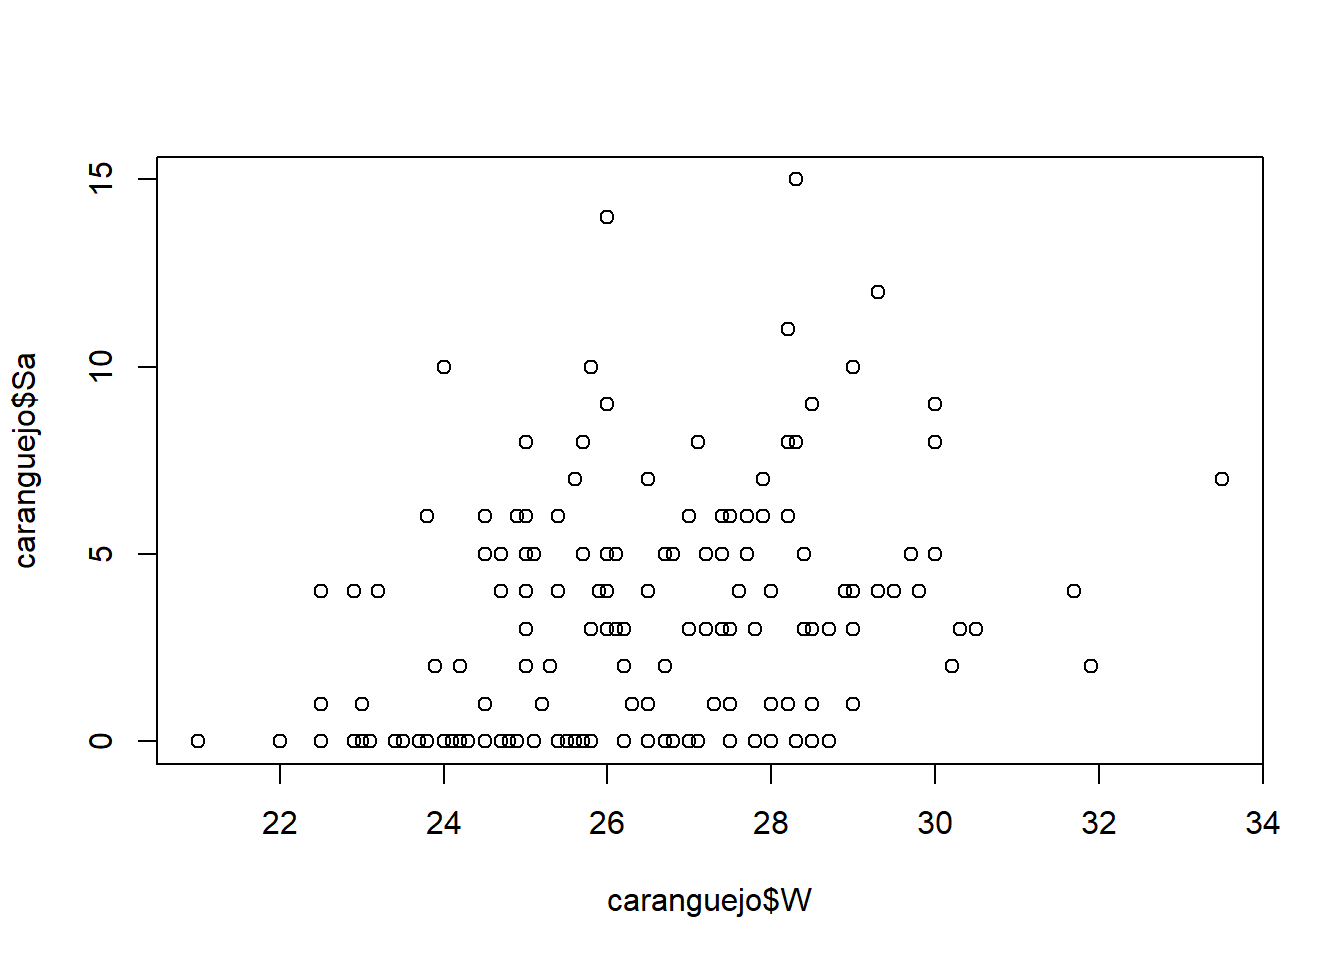
\includegraphics[width=0.8\linewidth]{index_files/figure-latex/unnamed-chunk-95-1} \end{center}

Relacionando a quantidade de satélites (Sa) com a largura da carapaça:

\begin{Shaded}
\begin{Highlighting}[]
\KeywordTok{plot}\NormalTok{(caranguejo}\OperatorTok{$}\NormalTok{W,caranguejo}\OperatorTok{$}\NormalTok{Sa)}
\end{Highlighting}
\end{Shaded}

\begin{center}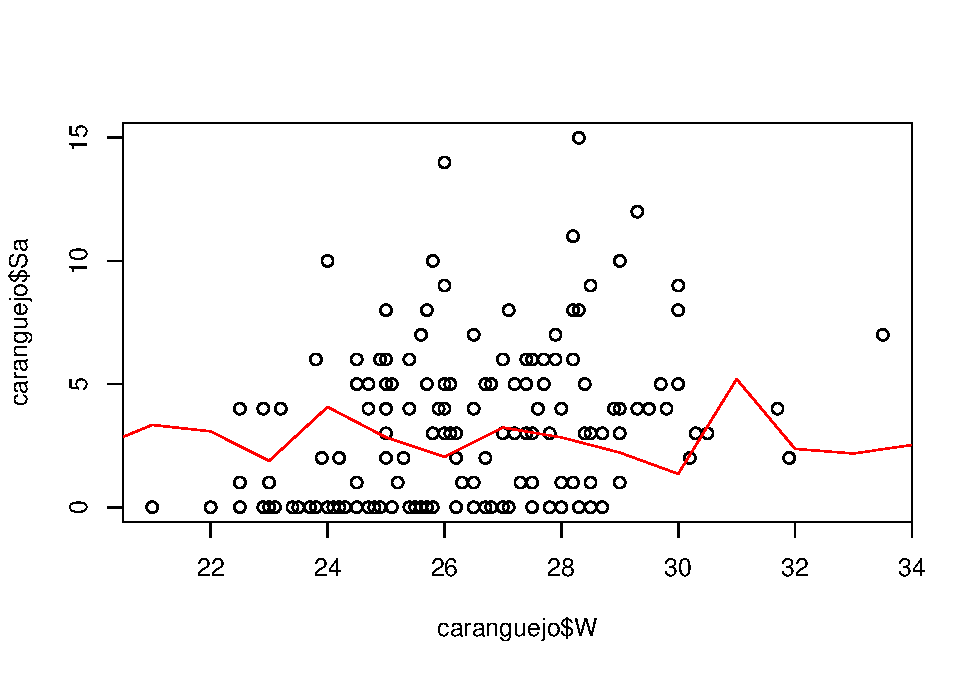
\includegraphics[width=0.8\linewidth]{index_files/figure-latex/unnamed-chunk-96-1} \end{center}

Para criação da regressão de Poisson utiliza-se a função já conhecida \texttt{glm()}, sendo que em \texttt{family} é determinado o tipo de análise desejada (``poisson''):

\begin{Shaded}
\begin{Highlighting}[]
\NormalTok{regpoisson=}\KeywordTok{glm}\NormalTok{(Sa}\OperatorTok{~}\NormalTok{W, }\DataTypeTok{family=}\StringTok{"poisson"}\NormalTok{, }\DataTypeTok{data=}\NormalTok{caranguejo)}
\KeywordTok{summary}\NormalTok{(regpoisson)}
\end{Highlighting}
\end{Shaded}

\begin{verbatim}

Call:
glm(formula = Sa ~ W, family = "poisson", data = caranguejo)

Deviance Residuals: 
   Min      1Q  Median      3Q     Max  
-2.853  -1.988  -0.493   1.097   4.922  

Coefficients:
            Estimate Std. Error z value Pr(>|z|)    
(Intercept)   -3.305      0.542   -6.09  1.1e-09 ***
W              0.164      0.020    8.22  < 2e-16 ***
---
Signif. codes:  0 '***' 0.001 '**' 0.01 '*' 0.05 '.' 0.1 ' ' 1

(Dispersion parameter for poisson family taken to be 1)

    Null deviance: 632.79  on 172  degrees of freedom
Residual deviance: 567.88  on 171  degrees of freedom
AIC: 927.2

Number of Fisher Scoring iterations: 6
\end{verbatim}

O modelo estimado:

\[
log(\hat\mu {/t}) = -3.30476 + 0,16405 W_i
\]
ou

\[
E(Y)= e^{-3.30476} + e^{0,16405 W_i}
\]

A leitura do resultado da regressão em geral se assemelha com os modelos de regressão linear e múltipla. Os resultados mostram que a largura da carapaça (W) tem relação positiva com o número de satélites (Sa) em volta do caranguejo fêmea, possuindo significância estatística a \(p=0,001\).

A interpretação do parâmetro \(0,16405W_i\):

\begin{itemize}
\item
  \textbf{(a)} como o parâmetro \(\beta_1\) é positivo, há uma relação positiva entre oa largura da carapaça (W) e o número de satélites (sa) esperados.
\item
  \textbf{(b)} exp(0,16405) = 1,178273. Logo, para cada elevação unitária na largura da carapaça (W) dos caranguejos, eleva-se em 1,178273 vezes o número de satélites (Sa).
\end{itemize}

Teste de dispersão:

\begin{Shaded}
\begin{Highlighting}[]
\KeywordTok{require}\NormalTok{(AER)}
\KeywordTok{dispersiontest}\NormalTok{(regpoisson)}
\end{Highlighting}
\end{Shaded}

\begin{verbatim}

    Overdispersion test

data:  regpoisson
z = 5.6, p-value = 1e-08
alternative hypothesis: true dispersion is greater than 1
sample estimates:
dispersion 
     3.157 
\end{verbatim}

\begin{itemize}
\tightlist
\item
  \textbf{(c)} O parâmetro de super-dispersão para esta equação é maior que 1. Sempre que for muito superior a 1 há vestígios de super-disposição no modelo.
\end{itemize}

Abaixo a análise de variância.

\begin{Shaded}
\begin{Highlighting}[]
\KeywordTok{anova}\NormalTok{(regpoisson, }\DataTypeTok{test=}\StringTok{"Chisq"}\NormalTok{)}
\end{Highlighting}
\end{Shaded}

\begin{verbatim}
Analysis of Deviance Table

Model: poisson, link: log

Response: Sa

Terms added sequentially (first to last)

     Df Deviance Resid. Df Resid. Dev Pr(>Chi)    
NULL                   172        633             
W     1     64.9       171        568  7.8e-16 ***
---
Signif. codes:  0 '***' 0.001 '**' 0.01 '*' 0.05 '.' 0.1 ' ' 1
\end{verbatim}

Abaixo são incluídos os valores preditos \texttt{regpoisson\$fitted.values} juntamente com os dados originais.

\begin{Shaded}
\begin{Highlighting}[]
\NormalTok{print=}\KeywordTok{data.frame}\NormalTok{(caranguejo, }\DataTypeTok{pred=}\NormalTok{(regpoisson}\OperatorTok{$}\NormalTok{fitted.values))}
\KeywordTok{head}\NormalTok{(print)}
\end{Highlighting}
\end{Shaded}

\begin{verbatim}
  Obs C S    W   Wt Sa  pred
1   1 2 3 28.3 3.05  8 3.810
2   2 3 3 26.0 2.60  4 2.613
3   3 3 3 25.6 2.15  0 2.447
4   4 4 2 21.0 1.85  0 1.150
5   5 2 3 29.0 3.00  1 4.274
6   6 1 2 25.0 2.30  3 2.217
\end{verbatim}

É possível comparar a distribuição dos valores preditos decorrentes da utilização do modelo de regressão de Poisson com a amostra inicial da base de dados analisada:

\begin{Shaded}
\begin{Highlighting}[]
\KeywordTok{plot}\NormalTok{(caranguejo}\OperatorTok{$}\NormalTok{W,caranguejo}\OperatorTok{$}\NormalTok{Sa)}
\KeywordTok{points}\NormalTok{(regpoisson}\OperatorTok{$}\NormalTok{fitted.values,}\DataTypeTok{col=}\StringTok{'red'}\NormalTok{, }\DataTypeTok{type =} \StringTok{"l"}\NormalTok{)}
\end{Highlighting}
\end{Shaded}

\begin{figure}[H]

{\centering 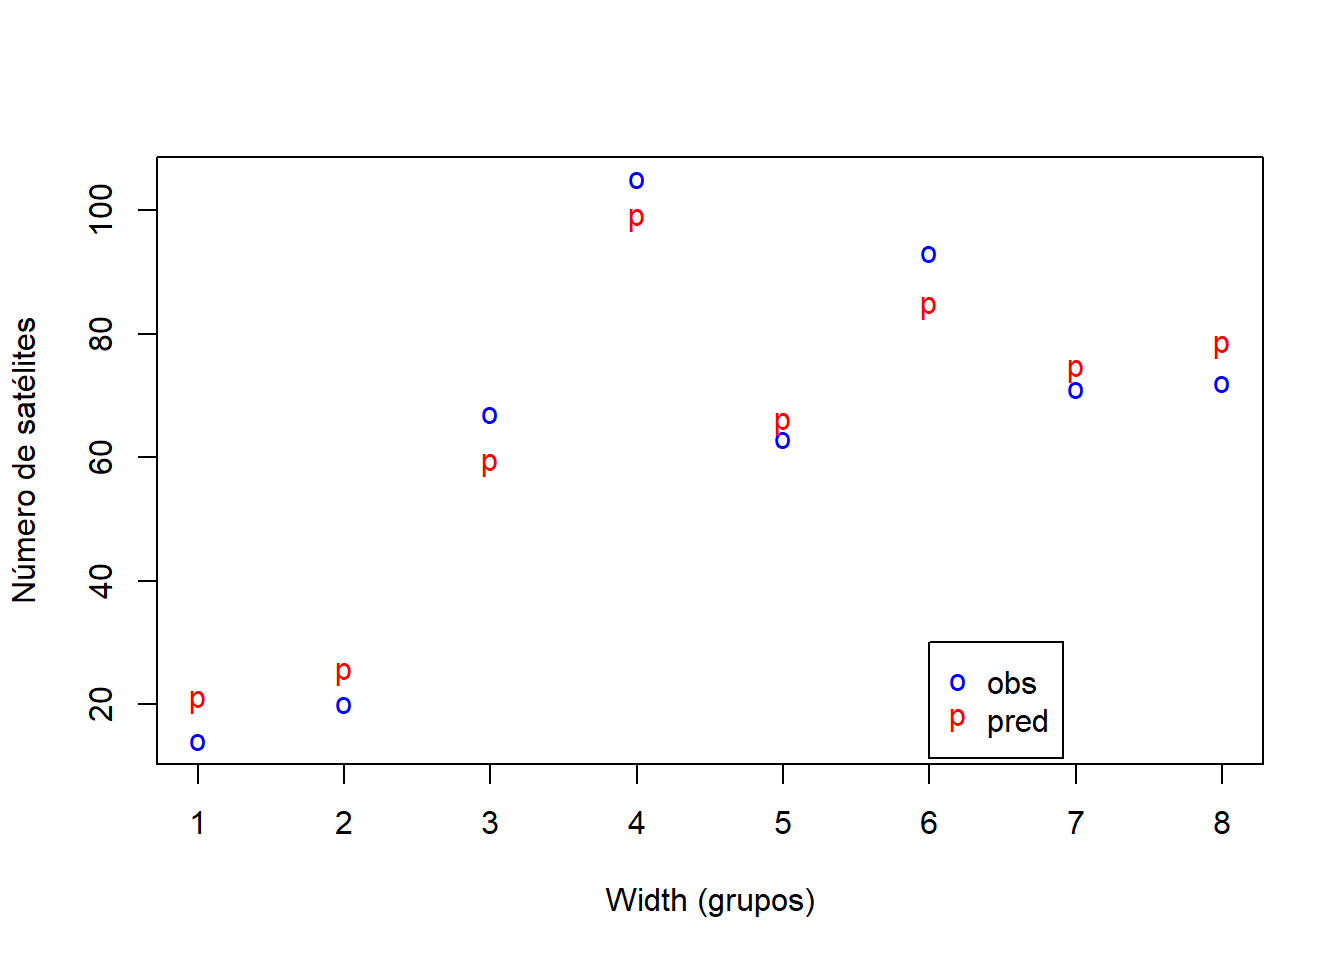
\includegraphics[width=0.8\linewidth]{index_files/figure-latex/unnamed-chunk-101-1} 

}

\caption{Valores ajustados e preditos do número de satélites (Sa) em função do tamanho da carapaça (W)}\label{fig:unnamed-chunk-101}
\end{figure}

No entanto, é possível melhorar a precisão do modelo de regressão utilizado, uma vez que os dados iniciais apresentam os casos individuais da amostra de cada caranguejo observado com suas respectivas características das variáveis independentes. Uma forma é agrupar os dados em intervalos da variável independente, contando os o número de casos (variável dependente) em cada intervalo.

Foram determinados 8 intervalos (``Intervalo'') conforme o tamanho da carapaça dos caranguejos. Contou-se o número de casos (variável ``numcasos'') de caranguejos em cada intervalo de tamanho da carapaça; o camanho médio da carapaça (``width'') em cada intervalo e; o número total de satélites (``satotal'') esperados em cada intervalo:

\begin{Shaded}
\begin{Highlighting}[]
\NormalTok{Intervalo=}\KeywordTok{c}\NormalTok{(}\StringTok{"<23,25"}\NormalTok{, }\StringTok{"23,25-24,25"}\NormalTok{,}\StringTok{"24,25-25,25"}\NormalTok{,}\StringTok{"25,25-26,25"}\NormalTok{,}
            \StringTok{"26,25-27,25"}\NormalTok{,}\StringTok{"27,25-28,25"}\NormalTok{,}\StringTok{"28,25-29,25"}\NormalTok{,}\StringTok{">29,25"}\NormalTok{)}
\KeywordTok{attach}\NormalTok{(caranguejo)}
\NormalTok{numcasos=}\KeywordTok{list}\NormalTok{(}\KeywordTok{length}\NormalTok{(}\KeywordTok{subset}\NormalTok{(W, W }\OperatorTok{<}\FloatTok{23.25}\NormalTok{)),}
              \KeywordTok{length}\NormalTok{(}\KeywordTok{subset}\NormalTok{(W, W }\OperatorTok{>}\FloatTok{23.25} \OperatorTok{&}\StringTok{ }\NormalTok{W }\OperatorTok{<}\FloatTok{24.25}\NormalTok{)),}
              \KeywordTok{length}\NormalTok{(}\KeywordTok{subset}\NormalTok{(W, W }\OperatorTok{>}\FloatTok{24.25} \OperatorTok{&}\StringTok{ }\NormalTok{W }\OperatorTok{<}\FloatTok{25.25}\NormalTok{)),}
              \KeywordTok{length}\NormalTok{(}\KeywordTok{subset}\NormalTok{(W, W }\OperatorTok{>}\FloatTok{25.25} \OperatorTok{&}\StringTok{ }\NormalTok{W }\OperatorTok{<}\FloatTok{26.25}\NormalTok{)),}
              \KeywordTok{length}\NormalTok{(}\KeywordTok{subset}\NormalTok{(W, W }\OperatorTok{>}\FloatTok{26.25} \OperatorTok{&}\StringTok{ }\NormalTok{W }\OperatorTok{<}\FloatTok{27.25}\NormalTok{)),}
              \KeywordTok{length}\NormalTok{(}\KeywordTok{subset}\NormalTok{(W, W }\OperatorTok{>}\FloatTok{27.25} \OperatorTok{&}\StringTok{ }\NormalTok{W }\OperatorTok{<}\FloatTok{28.25}\NormalTok{)),}
              \KeywordTok{length}\NormalTok{(}\KeywordTok{subset}\NormalTok{(W, W }\OperatorTok{>}\FloatTok{28.25} \OperatorTok{&}\StringTok{ }\NormalTok{W }\OperatorTok{<}\FloatTok{29.25}\NormalTok{)),}
              \KeywordTok{length}\NormalTok{(}\KeywordTok{subset}\NormalTok{(W, W }\OperatorTok{>}\FloatTok{29.25}\NormalTok{)))}
\NormalTok{width=}\KeywordTok{list}\NormalTok{(}\KeywordTok{mean}\NormalTok{(}\KeywordTok{subset}\NormalTok{(W, W }\OperatorTok{<}\FloatTok{23.25}\NormalTok{)),}
              \KeywordTok{mean}\NormalTok{(}\KeywordTok{subset}\NormalTok{(W, W }\OperatorTok{>}\FloatTok{23.25} \OperatorTok{&}\StringTok{ }\NormalTok{W }\OperatorTok{<}\FloatTok{24.25}\NormalTok{)),}
              \KeywordTok{mean}\NormalTok{(}\KeywordTok{subset}\NormalTok{(W, W }\OperatorTok{>}\FloatTok{24.25} \OperatorTok{&}\StringTok{ }\NormalTok{W }\OperatorTok{<}\FloatTok{25.25}\NormalTok{)),}
              \KeywordTok{mean}\NormalTok{(}\KeywordTok{subset}\NormalTok{(W, W }\OperatorTok{>}\FloatTok{25.25} \OperatorTok{&}\StringTok{ }\NormalTok{W }\OperatorTok{<}\FloatTok{26.25}\NormalTok{)),}
              \KeywordTok{mean}\NormalTok{(}\KeywordTok{subset}\NormalTok{(W, W }\OperatorTok{>}\FloatTok{26.25} \OperatorTok{&}\StringTok{ }\NormalTok{W }\OperatorTok{<}\FloatTok{27.25}\NormalTok{)),}
              \KeywordTok{mean}\NormalTok{(}\KeywordTok{subset}\NormalTok{(W, W }\OperatorTok{>}\FloatTok{27.25} \OperatorTok{&}\StringTok{ }\NormalTok{W }\OperatorTok{<}\FloatTok{28.25}\NormalTok{)),}
              \KeywordTok{mean}\NormalTok{(}\KeywordTok{subset}\NormalTok{(W, W }\OperatorTok{>}\FloatTok{28.25} \OperatorTok{&}\StringTok{ }\NormalTok{W }\OperatorTok{<}\FloatTok{29.25}\NormalTok{)),}
              \KeywordTok{mean}\NormalTok{(}\KeywordTok{subset}\NormalTok{(W, W }\OperatorTok{>}\FloatTok{29.25}\NormalTok{)))}
\NormalTok{satotal=}\KeywordTok{list}\NormalTok{(}\KeywordTok{sum}\NormalTok{(}\KeywordTok{subset}\NormalTok{(Sa, W }\OperatorTok{<}\FloatTok{23.25}\NormalTok{)),}
              \KeywordTok{sum}\NormalTok{(}\KeywordTok{subset}\NormalTok{(Sa, W }\OperatorTok{>}\FloatTok{23.25} \OperatorTok{&}\StringTok{ }\NormalTok{W }\OperatorTok{<}\FloatTok{24.25}\NormalTok{)),}
              \KeywordTok{sum}\NormalTok{(}\KeywordTok{subset}\NormalTok{(Sa, W }\OperatorTok{>}\FloatTok{24.25} \OperatorTok{&}\StringTok{ }\NormalTok{W }\OperatorTok{<}\FloatTok{25.25}\NormalTok{)),}
              \KeywordTok{sum}\NormalTok{(}\KeywordTok{subset}\NormalTok{(Sa, W }\OperatorTok{>}\FloatTok{25.25} \OperatorTok{&}\StringTok{ }\NormalTok{W }\OperatorTok{<}\FloatTok{26.25}\NormalTok{)),}
              \KeywordTok{sum}\NormalTok{(}\KeywordTok{subset}\NormalTok{(Sa, W }\OperatorTok{>}\FloatTok{26.25} \OperatorTok{&}\StringTok{ }\NormalTok{W }\OperatorTok{<}\FloatTok{27.25}\NormalTok{)),}
              \KeywordTok{sum}\NormalTok{(}\KeywordTok{subset}\NormalTok{(Sa, W }\OperatorTok{>}\FloatTok{27.25} \OperatorTok{&}\StringTok{ }\NormalTok{W }\OperatorTok{<}\FloatTok{28.25}\NormalTok{)),}
              \KeywordTok{sum}\NormalTok{(}\KeywordTok{subset}\NormalTok{(Sa, W }\OperatorTok{>}\FloatTok{28.25} \OperatorTok{&}\StringTok{ }\NormalTok{W }\OperatorTok{<}\FloatTok{29.25}\NormalTok{)),}
              \KeywordTok{sum}\NormalTok{(}\KeywordTok{subset}\NormalTok{(Sa, W }\OperatorTok{>}\FloatTok{29.25}\NormalTok{)))}
\NormalTok{numcasos <-}\StringTok{ }\KeywordTok{data.frame}\NormalTok{(}\KeywordTok{matrix}\NormalTok{(}\KeywordTok{unlist}\NormalTok{(numcasos), }\DataTypeTok{nrow=}\DecValTok{8}\NormalTok{, }\DataTypeTok{byrow=}\NormalTok{T),}
                       \DataTypeTok{stringsAsFactors=}\OtherTok{FALSE}\NormalTok{)}
\NormalTok{width <-}\StringTok{ }\KeywordTok{data.frame}\NormalTok{(}\KeywordTok{matrix}\NormalTok{(}\KeywordTok{unlist}\NormalTok{(width), }\DataTypeTok{nrow=}\DecValTok{8}\NormalTok{, }\DataTypeTok{byrow=}\NormalTok{T),}
                    \DataTypeTok{stringsAsFactors=}\OtherTok{FALSE}\NormalTok{)}
\NormalTok{satotal <-}\StringTok{ }\KeywordTok{data.frame}\NormalTok{(}\KeywordTok{matrix}\NormalTok{(}\KeywordTok{unlist}\NormalTok{(satotal), }\DataTypeTok{nrow=}\DecValTok{8}\NormalTok{, }\DataTypeTok{byrow=}\NormalTok{T),}
                      \DataTypeTok{stringsAsFactors=}\OtherTok{FALSE}\NormalTok{)}

\NormalTok{novosdados=}\KeywordTok{data.frame}\NormalTok{(Intervalo,numcasos,}\KeywordTok{round}\NormalTok{(width,}\DecValTok{2}\NormalTok{),satotal)}

\KeywordTok{names}\NormalTok{(novosdados)=}\KeywordTok{c}\NormalTok{(}\StringTok{"Intervalo"}\NormalTok{,}\StringTok{"numcasos"}\NormalTok{,}\StringTok{"width"}\NormalTok{,}\StringTok{"satotal"}\NormalTok{)}
\NormalTok{novosdados}
\end{Highlighting}
\end{Shaded}

\begin{verbatim}
    Intervalo numcasos width satotal
1      <23,25       14 22.69      14
2 23,25-24,25       14 23.84      20
3 24,25-25,25       28 24.77      67
4 25,25-26,25       39 25.84     105
5 26,25-27,25       22 26.79      63
6 27,25-28,25       24 27.74      93
7 28,25-29,25       18 28.67      71
8      >29,25       14 30.41      72
\end{verbatim}

Segue a especificação deste novo modelo agrupado. Segundo PENNSTATE (\protect\hyperlink{ref-penn2018}{2018}), utiliou-se o componente de ajuste da equação (\texttt{offset}) como o logarítmo do número de casos (``lcases''), como ``o valor de ajuste `t' no modelo que representa o espaço fixo, neste caso o grupo (caranguejos com largura similar)''. O resultado da nova regressão se mostra melhor ajustado, com redução do índice AIC:

\begin{Shaded}
\begin{Highlighting}[]
\CommentTok{# Log do Número de Casos}
\NormalTok{lcases=}\KeywordTok{log}\NormalTok{(numcasos) }
\CommentTok{# Incluir a varíavel anterior no objeto novosdados}
\NormalTok{novosdados=}\KeywordTok{data.frame}\NormalTok{(novosdados,lcases) }
\KeywordTok{names}\NormalTok{(novosdados)[}\DecValTok{5}\NormalTok{]=}\StringTok{"lcases"}
\NormalTok{model=}\KeywordTok{glm}\NormalTok{(satotal}\OperatorTok{~}\NormalTok{width, }\DataTypeTok{offset=}\NormalTok{lcases, }\DataTypeTok{family=}\StringTok{"poisson"}\NormalTok{, }\DataTypeTok{data=}\NormalTok{novosdados)}
\KeywordTok{summary}\NormalTok{(model)}
\end{Highlighting}
\end{Shaded}

\begin{verbatim}

Call:
glm(formula = satotal ~ width, family = "poisson", data = novosdados, 
    offset = lcases)

Deviance Residuals: 
   Min      1Q  Median      3Q     Max  
-1.533  -0.773  -0.345   0.712   1.039  

Coefficients:
            Estimate Std. Error z value Pr(>|z|)    
(Intercept)  -3.5355     0.5760   -6.14  8.4e-10 ***
width         0.1727     0.0212    8.13  4.1e-16 ***
---
Signif. codes:  0 '***' 0.001 '**' 0.01 '*' 0.05 '.' 0.1 ' ' 1

(Dispersion parameter for poisson family taken to be 1)

    Null deviance: 72.3772  on 7  degrees of freedom
Residual deviance:  6.5168  on 6  degrees of freedom
AIC: 56.96

Number of Fisher Scoring iterations: 4
\end{verbatim}

A fórmula para esta nova regressão:

\[
log(\hat\mu/t)=-3.535 + 0,1727 width_i + log(t)
\]
Desta forma:

\begin{itemize}
\tightlist
\item
  \textbf{(a)} em conformidade com a equação anterior, o número esperado de satélites (satotal) cresce de acordo com o tamanho médio da carapaça dos caranguejos (width), pois o coeficiente é positivo.
\item
  \textbf{(b)} como exp(0,1727)=1,188509, espera-se que para cada alteração unitária no tamanho médio da carapaça dos caranguejos (width) eleve-se em 1,188509 vezes o número esperado de satélites (satotal).
\end{itemize}

Teste de super-dispersão:

\begin{Shaded}
\begin{Highlighting}[]
\KeywordTok{require}\NormalTok{(AER)}
\KeywordTok{dispersiontest}\NormalTok{(model)}
\end{Highlighting}
\end{Shaded}

\begin{verbatim}

    Overdispersion test

data:  model
z = -0.66, p-value = 0.7
alternative hypothesis: true dispersion is greater than 1
sample estimates:
dispersion 
    0.8273 
\end{verbatim}

\begin{itemize}
\tightlist
\item
  \textbf{(c)} o tesde de superdispersão aprovou a hipótese nula (\(p>0,05\)) de que não há problemas de super-dispersão no modelo.
\end{itemize}

Abaixo a análise de variância:

\begin{Shaded}
\begin{Highlighting}[]
\KeywordTok{anova}\NormalTok{(model, }\DataTypeTok{test=}\StringTok{"Chisq"}\NormalTok{)}
\end{Highlighting}
\end{Shaded}

\begin{verbatim}
Analysis of Deviance Table

Model: poisson, link: log

Response: satotal

Terms added sequentially (first to last)

      Df Deviance Resid. Df Resid. Dev Pr(>Chi)    
NULL                      7       72.4             
width  1     65.9         6        6.5  4.8e-16 ***
---
Signif. codes:  0 '***' 0.001 '**' 0.01 '*' 0.05 '.' 0.1 ' ' 1
\end{verbatim}

Abaixo demonstra-se a plotagem dos valores originais e preditos com a regressão de Poisson:

\begin{Shaded}
\begin{Highlighting}[]
\KeywordTok{plot}\NormalTok{(novosdados}\OperatorTok{$}\NormalTok{satotal, }\DataTypeTok{pch=}\StringTok{"o"}\NormalTok{, }\DataTypeTok{col=}\StringTok{"blue"}\NormalTok{, }\DataTypeTok{xlab=}\StringTok{"Width (grupos)"}\NormalTok{,}
     \DataTypeTok{ylab=}\StringTok{"Número de satélites"}\NormalTok{)}
\KeywordTok{points}\NormalTok{(model}\OperatorTok{$}\NormalTok{fitted.values, }\DataTypeTok{pch=}\StringTok{"p"}\NormalTok{, }\DataTypeTok{col=}\StringTok{"red"}\NormalTok{)}
\KeywordTok{legend}\NormalTok{(}\DecValTok{6}\NormalTok{,}\DecValTok{30}\NormalTok{,}\KeywordTok{c}\NormalTok{(}\StringTok{"obs"}\NormalTok{,}\StringTok{"pred"}\NormalTok{), }\DataTypeTok{pch=}\KeywordTok{c}\NormalTok{(}\StringTok{"o"}\NormalTok{,}\StringTok{"p"}\NormalTok{), }\DataTypeTok{col=}\KeywordTok{c}\NormalTok{(}\StringTok{"blue"}\NormalTok{,}\StringTok{"red"}\NormalTok{))}
\end{Highlighting}
\end{Shaded}

\begin{figure}[H]

{\centering 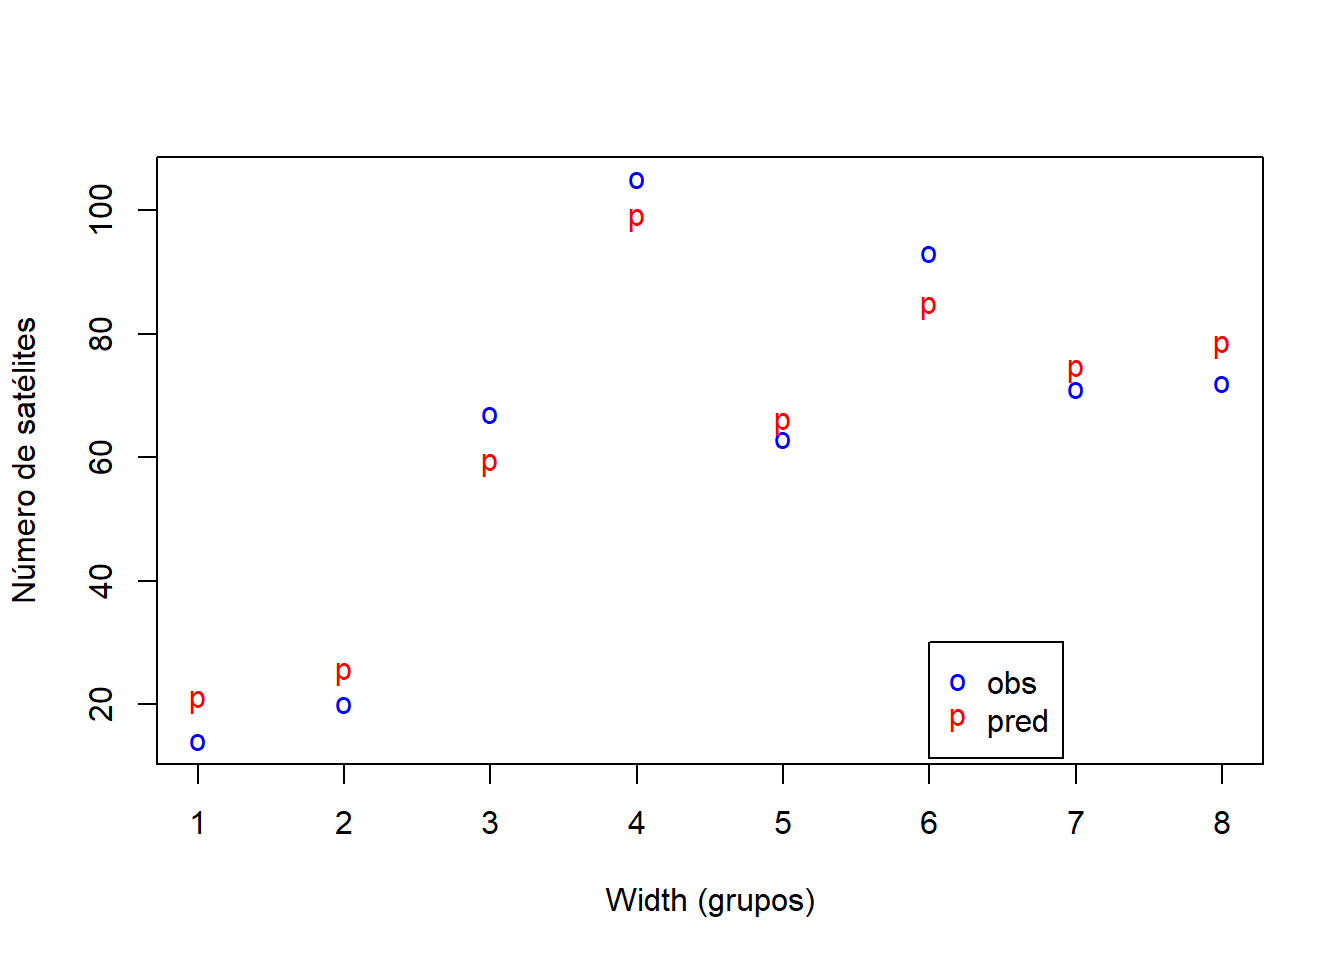
\includegraphics[width=0.8\linewidth]{index_files/figure-latex/unnamed-chunk-106-1} 

}

\caption{Valores observados e preditos}\label{fig:unnamed-chunk-106}
\end{figure}

Fonte: Adaptado de PENNSTATE (\protect\hyperlink{ref-penn2018}{2018}).

\begin{Shaded}
\begin{Highlighting}[]
\NormalTok{novosdados}\OperatorTok{$}\NormalTok{pred=model}\OperatorTok{$}\NormalTok{fitted.values}
\KeywordTok{head}\NormalTok{(novosdados)}
\end{Highlighting}
\end{Shaded}

\begin{verbatim}
    Intervalo numcasos width satotal lcases  pred
1      <23,25       14 22.69      14  2.639 20.54
2 23,25-24,25       14 23.84      20  2.639 25.06
3 24,25-25,25       28 24.77      67  3.332 58.85
4 25,25-26,25       39 25.84     105  3.664 98.61
5 26,25-27,25       22 26.79      63  3.091 65.54
6 27,25-28,25       24 27.74      93  3.178 84.25
\end{verbatim}

Alguns procedimentos usuais para avaliar a qualidade do modelo e ajuste dos dados da regressão de Poisson:

\begin{itemize}
\tightlist
\item
  Análise de resíudos;
\item
  Análise de pontos influentes;
\item
  Análise de variância;
\item
  Indicador AIC;
\item
  Análise de super-dispersão do modelo (quando Var(Y) \textgreater{} E(Y)). Neste caso, pode ocorrer por três motivos: a) função de ligação inadequada: talvez outras funções além da logarítimica se ajustem melhor; b) não inclusão de variáveis relevantes ao modelo; c) excessos de zeros.
\end{itemize}

\hypertarget{manipulando-bases-de-dados}{%
\chapter{Manipulando bases de dados}\label{manipulando-bases-de-dados}}

\emph{Felipe Micail da Silva Smolski}

O objetivo deste capítulo é retomar alguns pacotes importantes no RStudio para a
manipulação e transformação de grandes bases de dados que o pesquisador terá que manejar ao longo dos processos de análise.

\hypertarget{pacote-tidyr}{%
\section{Pacote tidyr}\label{pacote-tidyr}}

Nesta seção será utilizado o pacote \texttt{tidyr} para demonstrar algumas funções no tocante da manipulação das bases de dados, tão importante no processo de preperação das informações para posterior análise. Serão utilizadas para demonstração as bases de dados existentes no próprio pacote.

Abaixo segue uma demonstração das convenções a respeito das bases de dados. Desta forma verifica-se que cada variável é apresentada em sua respectiva coluna, bem como as observações são apresentadas em sua própria linha e portanto os valores constam em sua própria célula.

\begin{figure}[H]

{\centering 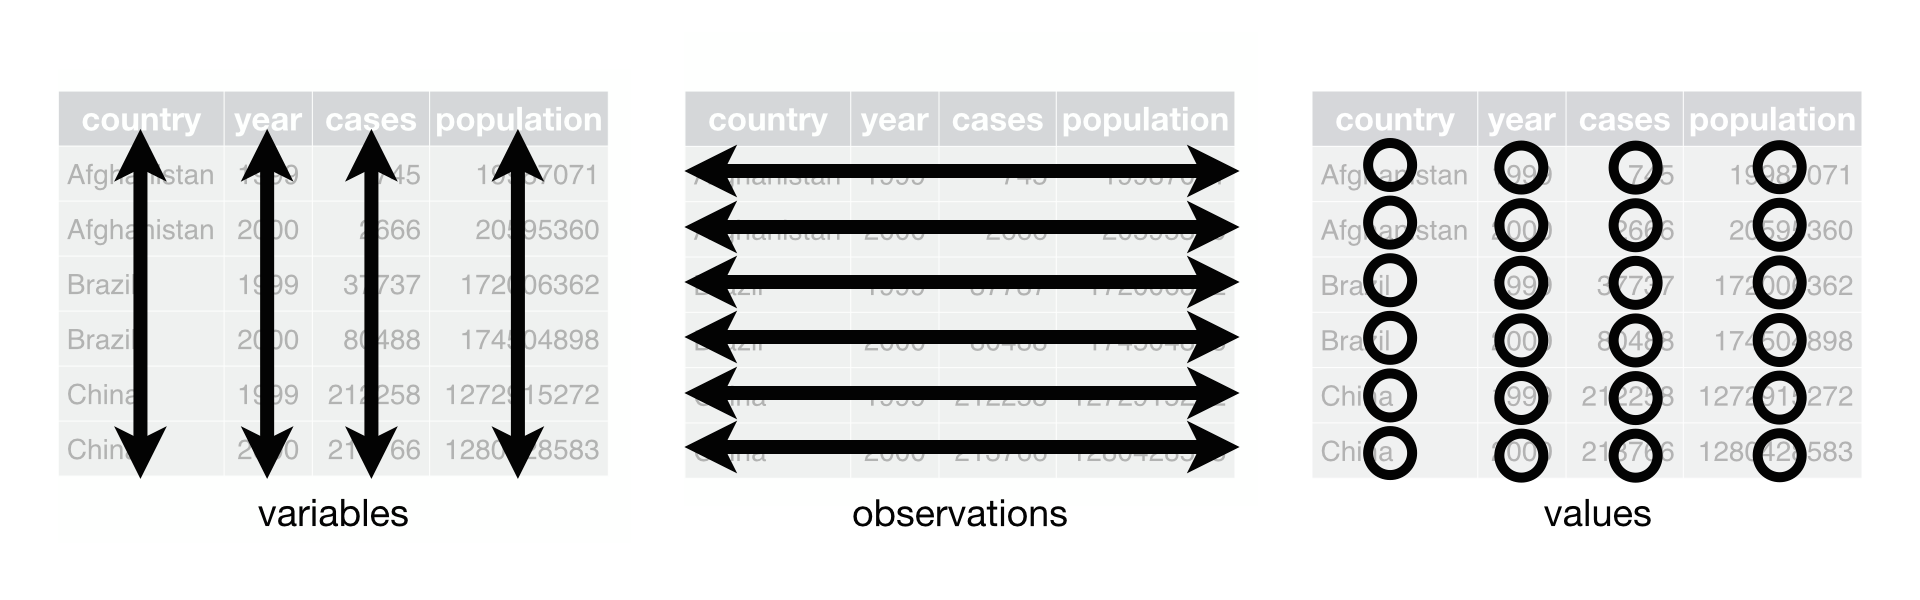
\includegraphics[width=0.8\linewidth]{tidy-1} 

}

\caption{Convenção sobre variáveis, observações e valores}\label{fig:dados}
\end{figure}

\hypertarget{funcao-spread}{%
\subsection{\texorpdfstring{Função \emph{spread}}{Função spread}}\label{funcao-spread}}

A função \emph{spread} é utilizada para transformar os valores constantes em uma coluna em nova configuração de colunas. Ainda, é possível determinar a transformação dos valores com o comando \texttt{convert\ =\ TRUE} informando o tipo de valores (doubles (numerics), integers, logicals, complexes, ou factors) nas colunas a serem criadas (comando \texttt{type.convert()}).

\begin{Shaded}
\begin{Highlighting}[]
\KeywordTok{require}\NormalTok{(tidyr)}
\end{Highlighting}
\end{Shaded}

\begin{verbatim}
Carregando pacotes exigidos: tidyr
\end{verbatim}

\begin{Shaded}
\begin{Highlighting}[]
\NormalTok{table1}
\end{Highlighting}
\end{Shaded}

\begin{verbatim}
# A tibble: 6 x 4
  country      year  cases population
  <chr>       <int>  <int>      <int>
1 Afghanistan  1999    745   19987071
2 Afghanistan  2000   2666   20595360
3 Brazil       1999  37737  172006362
4 Brazil       2000  80488  174504898
5 China        1999 212258 1272915272
6 China        2000 213766 1280428583
\end{verbatim}

Neste exemplo, a coluna \texttt{type} abriga os valores \texttt{cases} e \texttt{population}, as quais terão suas próprias colunas com seus respectivos valores:

\begin{Shaded}
\begin{Highlighting}[]
\KeywordTok{spread}\NormalTok{(table2, type, count)}
\end{Highlighting}
\end{Shaded}

\begin{verbatim}
# A tibble: 6 x 4
  country      year  cases population
  <chr>       <int>  <int>      <int>
1 Afghanistan  1999    745   19987071
2 Afghanistan  2000   2666   20595360
3 Brazil       1999  37737  172006362
4 Brazil       2000  80488  174504898
5 China        1999 212258 1272915272
6 China        2000 213766 1280428583
\end{verbatim}

\hypertarget{funcao-gather}{%
\subsection{\texorpdfstring{Função \emph{gather}}{Função gather}}\label{funcao-gather}}

Já a função \emph{gather} realiza o processo oposto do comando \emph{spread}, pois agrupa o valor de determinadas variável em uma chave comum.

\begin{Shaded}
\begin{Highlighting}[]
\NormalTok{table4a}
\end{Highlighting}
\end{Shaded}

\begin{verbatim}
# A tibble: 3 x 3
  country     `1999` `2000`
* <chr>        <int>  <int>
1 Afghanistan    745   2666
2 Brazil       37737  80488
3 China       212258 213766
\end{verbatim}

Abaixo a transformação das variáveis \texttt{1999} e \texttt{2000} em uma única variável \texttt{year}, mantendo os valores inseridos na variável \texttt{cases}:

\begin{Shaded}
\begin{Highlighting}[]
\KeywordTok{gather}\NormalTok{(table4a, }\StringTok{"year"}\NormalTok{, }\StringTok{"cases"}\NormalTok{, }\DecValTok{2}\OperatorTok{:}\DecValTok{3}\NormalTok{)}
\end{Highlighting}
\end{Shaded}

\begin{verbatim}
# A tibble: 6 x 3
  country     year   cases
  <chr>       <chr>  <int>
1 Afghanistan 1999     745
2 Brazil      1999   37737
3 China       1999  212258
4 Afghanistan 2000    2666
5 Brazil      2000   80488
6 China       2000  213766
\end{verbatim}

\hypertarget{funcao-separate}{%
\subsection{\texorpdfstring{Função \emph{separate}}{Função separate}}\label{funcao-separate}}

A função \emph{separate} é utilizada para partir uma determinada variável em novas variáveis da base de dados.

\begin{Shaded}
\begin{Highlighting}[]
\NormalTok{table3}
\end{Highlighting}
\end{Shaded}

\begin{verbatim}
# A tibble: 6 x 3
  country      year rate             
* <chr>       <int> <chr>            
1 Afghanistan  1999 745/19987071     
2 Afghanistan  2000 2666/20595360    
3 Brazil       1999 37737/172006362  
4 Brazil       2000 80488/174504898  
5 China        1999 212258/1272915272
6 China        2000 213766/1280428583
\end{verbatim}

Neste exemplo, a variável \texttt{rate}, que está composta de duas informações separadas pelo caractere ``\(/\)'', será separada nas novas variáveis \texttt{cases} e \texttt{population}:

\begin{Shaded}
\begin{Highlighting}[]
\KeywordTok{separate}\NormalTok{(table3, rate, }\DataTypeTok{into =} \KeywordTok{c}\NormalTok{(}\StringTok{"cases"}\NormalTok{, }\StringTok{"population"}\NormalTok{),}\DataTypeTok{sep =} \StringTok{"/"}\NormalTok{)}
\end{Highlighting}
\end{Shaded}

\begin{verbatim}
# A tibble: 6 x 4
  country      year cases  population
* <chr>       <int> <chr>  <chr>     
1 Afghanistan  1999 745    19987071  
2 Afghanistan  2000 2666   20595360  
3 Brazil       1999 37737  172006362 
4 Brazil       2000 80488  174504898 
5 China        1999 212258 1272915272
6 China        2000 213766 1280428583
\end{verbatim}

Da mesma forma é possível criar duas novas variáveis a partir do segundo caractere do valor que consta nas células utilizando o comando \texttt{sep=2}:

\begin{Shaded}
\begin{Highlighting}[]
\KeywordTok{separate}\NormalTok{(table3, year, }\DataTypeTok{into =} \KeywordTok{c}\NormalTok{(}\StringTok{"century"}\NormalTok{, }\StringTok{"year"}\NormalTok{), }\DataTypeTok{sep =} \DecValTok{2}\NormalTok{)}
\end{Highlighting}
\end{Shaded}

\begin{verbatim}
# A tibble: 6 x 4
  country     century year  rate             
* <chr>       <chr>   <chr> <chr>            
1 Afghanistan 19      99    745/19987071     
2 Afghanistan 20      00    2666/20595360    
3 Brazil      19      99    37737/172006362  
4 Brazil      20      00    80488/174504898  
5 China       19      99    212258/1272915272
6 China       20      00    213766/1280428583
\end{verbatim}

\hypertarget{funcao-unite}{%
\subsection{\texorpdfstring{Função \emph{unite}}{Função unite}}\label{funcao-unite}}

A função \texttt{unite} é oposta à função \emph{separate}:

\begin{Shaded}
\begin{Highlighting}[]
\NormalTok{table5}
\end{Highlighting}
\end{Shaded}

\begin{verbatim}
# A tibble: 6 x 4
  country     century year  rate             
* <chr>       <chr>   <chr> <chr>            
1 Afghanistan 19      99    745/19987071     
2 Afghanistan 20      00    2666/20595360    
3 Brazil      19      99    37737/172006362  
4 Brazil      20      00    80488/174504898  
5 China       19      99    212258/1272915272
6 China       20      00    213766/1280428583
\end{verbatim}

Neste exemplo, recria a variável \texttt{new} a partir dos dados de \texttt{century} e \texttt{year}:

\begin{Shaded}
\begin{Highlighting}[]
\KeywordTok{unite}\NormalTok{(table5, }\StringTok{"new"}\NormalTok{, century, year, }\DataTypeTok{sep =} \StringTok{""}\NormalTok{)}
\end{Highlighting}
\end{Shaded}

\begin{verbatim}
# A tibble: 6 x 3
  country     new   rate             
  <chr>       <chr> <chr>            
1 Afghanistan 1999  745/19987071     
2 Afghanistan 2000  2666/20595360    
3 Brazil      1999  37737/172006362  
4 Brazil      2000  80488/174504898  
5 China       1999  212258/1272915272
6 China       2000  213766/1280428583
\end{verbatim}

\hypertarget{pacote-dplyr}{%
\section{Pacote dplyr}\label{pacote-dplyr}}

\setlength{\parindent}{0.0cm}

\RaggedRight

\frenchspacing

\hypertarget{referencias}{%
\chapter*{Referências}\label{referencias}}
\addcontentsline{toc}{chapter}{Referências}

\hypertarget{refs}{}
\leavevmode\hypertarget{ref-breusch1978}{}%
BREUSCH, T. S. \textbf{Testing for autocorrelation in dynamic linear models}. \emph{Australian Economic Papers}, {[}s.l.{]}, n. 31, 1978.

\leavevmode\hypertarget{ref-breusch1979}{}%
BREUSCH, T. S.; PAGAN, A. R. \textbf{A simple test for heteroscedasticity and random coefficient variation}. \emph{Econometrica: Journal of the Econometric Society}, {[}s.l.{]}, 1979.

\leavevmode\hypertarget{ref-breusch1980}{}%
BREUSCH, T. S.; PAGAN, A. R. \textbf{The Lagrange multiplier test and its applications to model specification in econometrics}. \emph{The Review of Economic Studies}, {[}s.l.{]}, n. 1, 1980.

\leavevmode\hypertarget{ref-Fawcett2006}{}%
FAWCETT, T. \textbf{An introduction to ROC analysis}. \emph{Pattern Recognition Letters}, {[}s.l.{]}, 2006.

\leavevmode\hypertarget{ref-Gujarati2011}{}%
GUJARATI, D. N.; PORTER, D. C. \textbf{Econometria básica}. New York: Mc Graw Hill, 2011.

\leavevmode\hypertarget{ref-Hair2009}{}%
HAIR, J. F. et al. \textbf{Análise Multivariada de Dados}. São Paulo: Bookman, 2009.

\leavevmode\hypertarget{ref-hausman1978}{}%
HAUSMAN, J. A. \textbf{Specification tests in econometrics}. \emph{Econometrica: Journal of the econometric society}, {[}s.l.{]}, 1978.

\leavevmode\hypertarget{ref-Hosmer2000}{}%
HOSMER, D. W.; LEMESCHOW, S. \textbf{Applied Logistic Regression}. New York: Wiley, 2000.

\leavevmode\hypertarget{ref-Kassambara2017}{}%
KASSAMBARA, A. \textbf{Practical Guide To Cluster Analysis in R}. USA: CreateSpace: North Charleston, 2017.

\leavevmode\hypertarget{ref-penn2018}{}%
PENNSTATE. \textbf{R - Poisson Regression Model for Count Data}. 2018.

\leavevmode\hypertarget{ref-pesaran2015}{}%
PESARAN, M. H. \textbf{Testing weak cross-sectional dependence in large panels}. \emph{Econometric Reviews}, {[}s.l.{]}, n. 6-10, 2015.

\leavevmode\hypertarget{ref-Rawlings1998}{}%
RAWLINGS, J. O.; PANTULA, S. G.; DICKEY, D. A. \textbf{Applied Regression Analysis: A Research Tool}. New York: Springer, 1998.

\leavevmode\hypertarget{ref-Riboldi2005}{}%
RIBOLDI, J. \textbf{Modelos Lineares: notas de aula}. UFRGS: Programa de Pós-Graduação em Epidemiologia. Faculdade de Medicina, 2005.

\leavevmode\hypertarget{ref-Siegel2017}{}%
SIEGEL, E. \textbf{Análise Preditiva: O poder de prever quem vai clicar, comprar, mentir ou morrer}. Rio de Janeiro: Alta Books, 2017.

\leavevmode\hypertarget{ref-Torres-Reyna2014}{}%
TORRES-REYNA, O. \textbf{Logit, Probit and Multinomial Logit models in R}. 2014.

\leavevmode\hypertarget{ref-wooldridge2010}{}%
WOOLDRIDGE, J. M. \textbf{Econometric analysis of cross section and panel data}. {[}s.l.{]}: MIT Press, 2010.


\end{document}
